% !TEX program = xelatex
\documentclass[a4paper, 11pt]{article}

% ==========================
% HỖ TRỢ TIẾNG VIỆT & FONT (XELATEX)
% ==========================
\usepackage[vietnamese]{babel}
\usepackage{fontspec}
\setmainfont{TeX Gyre Termes}

% ==========================
% BỐ CỤC TRANG & TOÁN HỌC
% ==========================
\usepackage[margin=2.5cm]{geometry}
\usepackage{amsmath, amssymb, amsfonts}

% ==========================
% HÌNH ẢNH & MÀU SẮC
% ==========================
\usepackage{graphicx}
\usepackage{float}
\usepackage[table]{xcolor}

% ==========================
% BẢNG BIỂU
% ==========================
\usepackage{array}
\usepackage{tabularx}
\usepackage{booktabs}
\usepackage{multirow}
\usepackage{makecell}
\usepackage{longtable}

\newcolumntype{Y}{>{\raggedright\arraybackslash}X}

% ==========================
% DANH SÁCH & LIỆT KÊ
% ==========================
\usepackage{enumitem}
\setlist[itemize]{leftmargin=1.2em,itemsep=0.1em,topsep=0.15em}
\setlist[enumerate]{leftmargin=1.2em,itemsep=0.1em,topsep=0.15em}
\setlength{\parindent}{0pt}
\setlength{\parskip}{0.35em}

% ==========================
% TIKZ & ĐỒ HỌA
% ==========================
\usepackage{tikz}
\usetikzlibrary{shapes.geometric, arrows, positioning, calc, decorations, backgrounds}

% ==========================
% CAPTION & SUB-CAPTION
% ==========================
\usepackage{caption}
\usepackage{subcaption}

% ==========================
% THUẬT TOÁN (ALGORITHM)
% ==========================
\usepackage[lined,boxed,commentsnumbered]{algorithm2e}

% ==========================
% KHUNG & HỘP (TCOLORBOX & MDFRAMED)
% ==========================
\usepackage[framemethod=tikz]{mdframed}
\usepackage[most]{tcolorbox}

\definecolor{deepgreen}{HTML}{2F4A17}
\definecolor{maingreen}{HTML}{6EAD42}
\definecolor{softgreen}{HTML}{EAF4E4}
\definecolor{cream}{HTML}{FAF8EF}
\definecolor{warning}{HTML}{C45A2A}
\definecolor{graytext}{HTML}{4B4B4B}

\newtcolorbox{keybox}[1]{
    enhanced,
    colback=softgreen,
    colframe=maingreen,
    coltitle=white,
    colbacktitle=deepgreen,
    title=\textbf{#1},
    arc=2mm,
    boxrule=0.7pt,
    left=1mm,
    right=1mm,
    top=1mm,
    bottom=1mm
}

\newtcolorbox{warnbox}[1]{
    enhanced,
    colback=cream,
    colframe=warning,
    coltitle=white,
    colbacktitle=warning,
    title=\textbf{#1},
    arc=2mm,
    boxrule=0.7pt,
    left=1mm,
    right=1mm,
    top=1mm,
    bottom=1mm
}

% ==========================
% CODE LISTING
% ==========================
\usepackage{listings}
\definecolor{dkgreen}{rgb}{0,0.6,0}
\definecolor{gray}{rgb}{0.5,0.5,0.5}
\definecolor{mauve}{rgb}{0.58,0,0.82}

\lstset{
    frame=tb,
    language=matlab,
    basicstyle={\small\ttfamily},
    breaklines=true,
    keywordstyle=\color{blue},
    commentstyle=\color{dkgreen},
    stringstyle=\color{mauve},
    numbers=left,
    numbersep=4pt,
    numberstyle=\tiny\color{gray}
}

% ==========================
% ĐỊNH DẠNG TIÊU ĐỀ
% ==========================
\usepackage{titlesec}
\titlespacing*{\section}{0pt}{0.75em}{0.35em}
\titlespacing*{\subsection}{0pt}{0.55em}{0.25em}

% ==========================
% MỤC LỤC SÂU 4 CẤP
% ==========================
\setcounter{secnumdepth}{4}
\setcounter{tocdepth}{3}

\makeatletter
\newcounter{subsubsubsection}[subsubsection]
\renewcommand\thesubsubsubsection{\thesubsubsection.\@alph\c@subsubsubsection}
\newcommand\subsubsubsection{\@startsection{subsubsubsection}{4}{\z@}
       {-3.25ex\@plus -1ex \@minus -.2ex}
       {1.5ex \@plus .2ex}
       {\normalfont\normalsize\bfseries}}
\newcommand*\l@subsubsubsection{\@dottedtocline{3}{10.0em}{4.1em}}
\makeatother

% ==========================
% HEADER & FOOTER
% ==========================
\usepackage{fancyhdr}
\usepackage{lastpage}
\usepackage{microtype}
\setlength{\headheight}{40pt}

\pagestyle{fancy}
\fancyhead{} 
\fancyhead[L]{
 \begin{tabular}{rl}
    \begin{picture}(25,15)(0,0)
    \put(0,-8){
\includegraphics[width=8mm]{graphics/logo_uit.png}}
   \end{picture}&
	\begin{tabular}{l}
		\textbf{\ttfamily Vietnam National University - Ho Chi Minh City}\\
  	\textbf{\ttfamily University of Information Technology}
	\end{tabular}
 \end{tabular}
}
\fancyhead[R]{}

\fancyfoot{}
\fancyfoot[L]{\scriptsize \ttfamily CS231 Project Report}
\fancyfoot[R]{\scriptsize \ttfamily Trang \thepage/\pageref{LastPage}}

\renewcommand{\headrulewidth}{0.3pt}
\renewcommand{\footrulewidth}{0.3pt}

% ==========================
% HYPERLINK
% ==========================
\usepackage{url}
\usepackage[colorlinks=true, linkcolor=blue!80!black, citecolor=blue!80!black, urlcolor=blue!80!black, breaklinks, plainpages=false, pdfpagelabels=true]{hyperref}

% ==========================
% LAYOUT VÀ BÌA
% ==========================
\usepackage{style}
\thesislayout

\begin{document}

\coverpage

\cleardoublepage
\pagenumbering{roman}
\setcounter{page}{1}

\tableofcontents
\cleardoublepage

\phantomsection
\addcontentsline{toc}{section}{Lời cảm ơn}
\section*{Lời cảm ơn}

Lời đầu tiên, chúng em xin trân trọng gửi lời cảm ơn sâu sắc nhất đến thầy Mai Tiến Dũng, giảng viên phụ trách môn học Thị giác máy tính (CS231), đã tận tình truyền đạt những kiến thức chuyên môn quý báu, định hướng phương pháp nghiên cứu và luôn hỗ trợ, giải đáp thắc mắc cho chúng em trong suốt quá trình học tập và thực hiện đề tài.

Chúng em cũng xin chân thành cảm ơn Ban Giám hiệu Trường Đại học Công nghệ Thông tin, Đại học Quốc gia TP. Hồ Chí Minh cùng quý thầy cô Khoa Khoa học Máy tính đã tạo điều kiện học tập tốt nhất, cung cấp môi trường học thuật chuyên nghiệp để chúng em hoàn thành tốt đồ án môn học này.

Mặc dù nhóm chúng em đã nỗ lực hết mình với tinh thần làm việc nghiêm túc và cầu thị, song do giới hạn về mặt thời gian và kiến thức thực tế, báo cáo đồ án khó tránh khỏi những thiếu sót nhất định. Nhóm chúng em rất mong nhận được những nhận xét, góp ý quý báu từ thầy để đề tài ngày càng được hoàn thiện và có tính ứng dụng thực tiễn cao hơn.

\vspace{0.6cm}
\begin{flushright}
\textit{TP. Hồ Chí Minh, Học kỳ 1 -- Năm học 2026 -- 2027}\\[0.2cm]
\textbf{Nhóm sinh vi\^en thực hiện}\\[0.15cm]
Từ Lê Tuấn Anh (24520133)\\
Nguyễn Thanh Tân (24521581)
\end{flushright}

\vspace{0.8cm}
\subsection*{Bảng phân công nhiệm vụ và trách nhiệm thực hiện}
\addcontentsline{toc}{subsection}{Bảng phân công nhiệm vụ và trách nhiệm thực hiện}

Nhằm đảm bảo tính minh bạch, độc lập và chuyên sâu trong nghiên cứu, đồ án được phân chia nhiệm vụ đồng đều giữa hai thành viên ($50\% - 50\%$) theo hai trục tiếp cận bổ trợ cho nhau:

\begin{table}[H]
\centering
\small
\caption{Phân công nhiệm vụ chi tiết và tỷ lệ đóng góp của các thành viên.}
\label{tab:phan_cong}
\begin{tabularx}{\textwidth}{|p{3.2cm}|p{3.5cm}|Y|}
\hline
\textbf{Thành viên} & \textbf{Mô-đun phụ trách} & \textbf{Nội dung kỹ thuật cụ thể} \\
\hline
\textbf{Từ Lê Tuấn Anh}\newline MSSV: 24520133 & Mô-đun Định vị (YOLO11s) \& Thị giác truyền thống & 
-- Tiền huấn luyện (CCTSDB) và tinh chỉnh mô hình YOLO11s 1-Class (\texttt{sign}) để cắt ảnh ROI.\newline
-- Thiết kế chuỗi đặc trưng đa tầng $S0 \rightarrow S3$ (HSV Circular Shift, Tỷ lệ khung hình Aspect Ratio, Lưới không gian $2 \times 2$, HOG 9 hướng gradient).\newline
-- Tối ưu hóa bộ phân loại Support Vector Machine (SVM) với kernel RBF. \\
\hline
\textbf{Nguyễn Thanh Tân}\newline MSSV: 24521581 & Mô-đun Học sâu (CNN) \& Khung Đối chuẩn Đa tầng & 
-- Nghiên cứu, thiết kế và tối ưu mạng nơ-ron tích chập Enhanced LeNet-5 (PyTorch).\newline
-- Thiết lập pipeline tăng cường dữ liệu (Data Augmentation), tối ưu hóa hàm mất mát Cross-Entropy và Adam Optimizer kết hợp StepLR Scheduler.\newline
-- Xây dựng cơ chế chia tách Block Split theo chuỗi video liên tục (Zero Data Leakage), đo lường đối chuẩn 2 tầng (ROI \& Scene Benchmark). \\
\hline
\end{tabularx}
\end{table}

\textit{Ghi chú:} Trong toàn bộ nội dung báo cáo sau đây, các phương pháp và kết quả được trình bày dưới góc nhìn khoa học khách quan và thống nhất của toàn bộ nhóm nghiên cứu.


\cleardoublepage
\pagenumbering{arabic}
\setcounter{page}{1}

\section{Lý do và cơ sở thực hiện đề tài}
\label{sec:ly_do}

\subsection{Lý do thực hiện đề tài và tính cấp thiết}
\label{subsec:cap_thiet}

Trong bối cảnh phát triển mạnh mẽ của các hệ thống Hỗ trợ Lái xe Nâng cao (Advanced Driver Assistance Systems -- ADAS) và phương tiện tự hành (Autonomous Vehicles), bài toán \textbf{Nhận dạng Biển báo Giao thông (Traffic Sign Recognition -- TSR)} là một mắt xích cốt lõi bảo đảm an toàn vận hành. Một hệ thống TSR chính xác và kịp thời cho phép phương tiện phát hiện sớm các giới hạn tốc độ, hướng di chuyển bắt buộc và các cảnh báo nguy hiểm tiềm ẩn, từ đó chủ động cảnh báo người lái hoặc can thiệp điều khiển tự động để ngăn ngừa tai nạn giao thông.

Tại Việt Nam, việc triển khai bài toán TSR ngoài thực tế đối mặt với ba thách thức kỹ thuật đặc thù:

\begin{enumerate}
    \item \textbf{Đặc thù bối cảnh đường sá phức tạp và mật độ giao thông cao:} Biển báo giao thông tại Việt Nam có kích thước biểu kiến biến thiên cực kỳ rộng trên khung hình camera hành trình (từ cự ly xa chỉ đạt dưới $15 \times 15\text{ px}$ đến cự ly gần vượt quá $100 \times 100\text{ px}$). Đồng thời, biển báo thường xuyên bị che khuất một phần bởi tán cây, dây cáp viễn thông, xe tải lớn hoặc các biển quảng cáo thương mại có màu sắc tương tự.
    \item \textbf{Biến thiên quang học và hiện tượng trôi dạt màu sắc (Color Drift):} Khí hậu nhiệt đới nắng gắt gây ra hiện tượng phản xạ chói lóa (specular glare), bóng râm gắt che cắt ngang mặt biển báo hoặc điều kiện thiếu sáng ban đêm. Các yếu tố này làm suy giảm nghiêm trọng độ tin cậy của không gian màu RGB nguyên bản.
    \item \textbf{Ràng buộc tài nguyên tính toán trên thiết bị biên (Edge Computing Constraints):} Các vi xử lý nhúng trên xe cơ giới (như dòng NVIDIA Jetson, Raspberry Pi hoặc MCU chuyên dụng) bị giới hạn nghiêm ngặt về công suất tiêu thụ điện và băng thông bộ nhớ. Việc triển khai các mô hình học sâu khổng lồ (End-to-End One-Stage Detectors đa lớp) thường tiêu tốn quá nhiều tài nguyên, gây độ trễ lớn và không thể đáp ứng tần số suy luận thời gian thực ($\ge 30\text{ FPS}$).
\end{enumerate}

\subsection{Cơ sở khoa học và nguyên lý phân tách nhiệm vụ (Two-Stage Decoupling)}
\label{subsec:co_so_khoa_hoc}

Nhằm giải quyết triệt để sự đánh đổi giữa độ chính xác nhận dạng và tốc độ thời gian thực, đồ án đề xuất kiến trúc \textbf{Pipeline Lai Hai Giai Đoạn (Two-Stage Hybrid Architecture)} dựa trên nguyên lý phân tách trách nhiệm (Task Decoupling):

\begin{itemize}
    \item \textbf{Giai đoạn 1 (Candidate Localization -- Định vị vùng ứng viên):} Nhiệm vụ quét và phát hiện vật thể kích thước biến thiên trên toàn cảnh đường phố góc rộng là thế mạnh vượt trội của mạng nơ-ron học sâu hiện đại. Nhóm đề xuất huấn luyện mô hình \textbf{YOLO11s} ở chế độ 1 lớp duy nhất (\texttt{sign}). Bằng cách loại bỏ gánh nặng phân loại ngữ nghĩa chi tiết ở tầng phát hiện, mạng tối đa hóa tỷ lệ bao phủ (Detection Recall) và giảm thiểu chi phí tính toán, chỉ chịu trách nhiệm cung cấp các hộp bao ứng viên (Region of Interest -- ROI).
    \item \textbf{Giai đoạn 2 (Semantic Classification -- Phân loại ngữ nghĩa biển báo):} Dựa trên Quy chuẩn Kỹ thuật Quốc gia QCVN 41:2019/BGTVT, biển báo giao thông mang tính quy chuẩn hóa rất cao về màu sắc (đỏ, vàng, xanh) và hình học viền (tròn, tam giác đều, chữ nhật/vuông). Nhóm thiết kế và đối chuẩn song song hai mô-đun phân loại độc lập trên CPU:
    \begin{enumerate}
        \item \textit{Hướng tiếp cận Thị giác máy tính truyền thống:} Khai thác các đặc trưng toán học tường minh (Lọc màu HSV dịch pha vòng tròn, Lưới không gian $2 \times 2$, Gradient định hướng HOG) kết hợp bộ phân loại Support Vector Machine (SVM) với hàm nhân RBF siêu nhẹ.
        \item \textit{Hướng tiếp cận Học sâu hiện đại:} Thiết kế mạng nơ-ron tích chập tùy biến \textbf{Enhanced LeNet-5 (PyTorch)} với cấu trúc tối giản gồm 3 khối tích chập, tích hợp Batch Normalization và Dropout nhằm tự động trích xuất các biểu trưng trừu tượng mà vẫn bảo đảm suy luận siêu tốc.
    \end{enumerate}
\end{itemize}

\section{Phát biểu bài toán và mô hình hóa hệ thống}
\label{sec:phat_bieu_bai_toan}

\subsection{Phát biểu bài toán hình thức (Formal Problem Formulation)}
\label{subsec:phat_bieu_hinh_thuc}

Cho một khung hình ảnh đầu vào $\mathbf{I} \in \mathbb{R}^{H \times W \times 3}$ thu nhận từ camera hành trình phía trước phương tiện giao thông. Mục tiêu của hệ thống là giải quyết bài toán qua hai bài toán con tuần tự:

\begin{enumerate}
    \item \textbf{Bài toán Định vị (Localization):} Tìm tập hợp $K$ hộp bao (bounding box) $\mathcal{B}$ định vị các vùng chứa biển báo giao thông:
    \begin{equation}
        \mathcal{B} = \left\{ b_k = (x_1, y_1, x_2, y_2)_k \;\middle|\; \text{conf}_k \ge \tau_{\text{conf}}, \, k = 1, \dots, K \right\}
        \label{eq:localization}
    \end{equation}
    với ngưỡng tin cậy phát hiện $\tau_{\text{conf}} = 0.25$. Với mỗi hộp bao hợp lệ $b_k$, trích xuất vùng ảnh con tương ứng:
    \begin{equation}
        \mathbf{I}^{(k)}_{\text{crop}} = \mathbf{I}[y_1 : y_2, \, x_1 : x_2] \in \mathbb{R}^{h_k \times w_k \times 3}
        \label{eq:crop}
    \end{equation}

    \item \textbf{Bài toán Phân loại Đa lớp (Multi-Class Classification):} Với mỗi ảnh con $\mathbf{I}^{(k)}_{\text{crop}}$, bộ phân loại gán một nhãn lớp mục tiêu $\hat{y}_k \in \mathcal{C}$ cùng phân phối độ tin cậy $p_k \in [0, 1]$. Không gian nhãn $\mathcal{C}$ bao gồm 4 nhóm mục tiêu quy chuẩn:
    \begin{equation}
        \mathcal{C} = \left\{ \text{Bien\_Cam}, \, \text{Bien\_Nguy\_Hiem}, \, \text{Bien\_Hieu\_Lenh}, \, \text{Bien\_Chi\_Dan} \right\}
        \label{eq:classes}
    \end{equation}
\end{enumerate}

\subsection{Các ràng buộc kỹ thuật cốt lõi}
\label{subsec:rang_buoc_ky_thuat}

Hệ thống được thiết kế dưới hai ràng buộc thực tế nghiêm ngặt:

\begin{itemize}
    \item \textbf{Nguyên tắc chống rò rỉ dữ liệu tuyệt đối (Zero Data Leakage):} Vì dữ liệu camera hành trình được trích xuất từ các đoạn video liên tục, việc phân chia ngẫu nhiên (Random Split) từng khung hình sẽ khiến các khung hình liên tiếp $(t, t + 1)$ có mức độ tương đồng quang học $> 95\%$ bị phân tán đồng thời vào cả tập huấn luyện và kiểm thử. Hiện tượng này dẫn đến việc mô hình chỉ học vẹt các mẫu cục bộ (empirical memorization) và thổi phồng sai lệch kết quả đánh giá. Do đó, toàn bộ dữ liệu bắt buộc phải được phân chia theo khối video liên tục (Block Split).
    \item \textbf{Độ trễ thời gian thực trên CPU (Real-Time Latency Constraint):} Khâu suy luận phân loại trên mỗi ảnh crop phải đạt tốc độ $\ge 300\text{ FPS}$ (độ trễ $< 3.3\text{ ms}$) khi thực thi trên CPU đơn lõi, bảo đảm tổng thời gian của cả pipeline duy trì tần số phản hồi an toàn cho xe chạy ngoài thực địa.
\end{itemize}

\subsection{Sơ đồ kiến trúc luồng dữ liệu toàn trình}
\label{subsec:so_do_luong_du_lieu}

Hình~\ref{fig:e2e_pipeline_overview} mô tả luồng xử lý khái quát của hệ thống lai hai giai đoạn. Chi tiết đặc tả kỹ thuật từng khối xử lý cùng quy cách giao tiếp đầu vào/đầu ra giữa các mô-đun được trình bày chi tiết tại Mục~\ref{sec:phuong_phap} (Hình~\ref{fig:detailed_pipeline_block}).

\begin{figure}[H]
\centering
\resizebox{\textwidth}{!}{%
\begin{tikzpicture}[
    node distance=1.0cm and 0.6cm,
    block/.style={rectangle, draw=deepgreen, fill=softgreen, thick, rounded corners=2pt, align=center, minimum height=1cm, inner sep=5pt, font=\small},
    branch/.style={rectangle, draw=maingreen!80!black, fill=cream, thick, rounded corners=2pt, align=center, minimum height=0.9cm, inner sep=4pt, font=\small},
    line/.style={draw=deepgreen, ->, >=stealth, thick}
]
    \node [block] (input) {Ảnh Đường Phố\\(960$\times$540 / 1920$\times$1080)};
    \node [block, right=of input] (yolo) {Giai đoạn 1:\\YOLO11s 1-Class\\Detector (\texttt{sign})};
    \node [block, right=of yolo] (roi) {Tập Candidate Boxes\\\& Trích xuất ROI};
    \node [branch, above right=0.3cm and 0.6cm of roi] (trad) {Giai đoạn 2A: Truyền thống\\Color + Grid + HOG\\$\rightarrow$ SVM (RBF)};
    \node [branch, below right=0.3cm and 0.6cm of roi] (deep) {Giai đoạn 2B: Học sâu\\Enhanced LeNet-5\\(Mạng CNN PyTorch)};
    \node [block, right=4.2cm of roi] (output) {Kết quả Dự đoán:\\Hộp bao \& Nhãn nhóm};

    \path [line] (input) -- (yolo);
    \path [line] (yolo) -- (roi);
    \path [line] (roi.east) |- (trad.west);
    \path [line] (roi.east) |- (deep.west);
    \path [line] (trad.east) -| (output.north);
    \path [line] (deep.east) -| (output.south);
\end{tikzpicture}%
}
\caption{Sơ đồ luồng xử lý toàn trình của hệ thống Two-Stage Hybrid Traffic Sign Recognition.}
\label{fig:e2e_pipeline_overview}
\end{figure}

\subsection{Quy chuẩn phân nhóm biển báo theo QCVN 41:2019/BGTVT}
\label{subsec:qcvn_phan_nhom}

Bảng~\ref{tab:qcvn_groups} tổng hợp các đặc trưng hình học và màu sắc của 4 nhóm biển báo mục tiêu:

\begin{table}[H]
\centering
\small
\caption{Đặc trưng hình học và màu sắc 4 nhóm biển báo giao thông theo QCVN 41:2019.}
\label{tab:qcvn_groups}
\begin{tabularx}{\textwidth}{|c|p{3.2cm}|p{2cm}|p{2.8cm}|Y|}
\hline
\textbf{ID} & \textbf{Tên nhóm quy chuẩn} & \textbf{Mã hiệu} & \textbf{Hình dạng} & \textbf{Đặc trưng nhận diện quang học} \\
\hline
0 & \texttt{Bien\_Cam} & P.*, B.8a & Hình tròn & Viền đỏ, nền trắng hoặc xanh lam, biểu tượng màu đen \\
\hline
1 & \texttt{Bien\_Nguy\_Hiem} & W.* & Tam giác đều & Viền đỏ, nền vàng, biểu tượng đen \\
\hline
2 & \texttt{Bien\_Hieu\_Lenh} & R.* & Hình tròn & Nền xanh lam chủ đạo, biểu tượng hình vẽ màu trắng \\
\hline
3 & \texttt{Bien\_Chi\_Dan} & I.* & Chữ nhật / Vuông & Nền xanh lam chủ đạo, ký hiệu và chữ viết màu trắng \\
\hline
\end{tabularx}
\end{table}

\section{Phương pháp nghiên cứu và giải pháp đề xuất}
\label{sec:phuong_phap}

Nhằm hiện thực hóa nguyên lý phân tách trách nhiệm (Two-Stage Decoupling), hệ thống được cấu trúc thành một luồng xử lý tuần tự kết hợp rẽ nhánh mô-đun hóa cao độ. Hình~\ref{fig:detailed_pipeline_block} trực quan hóa chi tiết từng mắt xích xử lý, quy định chặt chẽ dữ liệu đầu vào và định dạng đầu ra của từng khối chức năng.

\begin{figure}[H]
\centering
\resizebox{\textwidth}{!}{%
\begin{tikzpicture}[
    node distance=0.9cm and 0.5cm,
    block/.style={rectangle, draw=deepgreen, fill=softgreen, thick, rounded corners=3pt, align=center, minimum height=1.2cm, inner sep=6pt, font=\small},
    branchA/.style={rectangle, draw=maingreen!90!black, fill=cream, thick, rounded corners=3pt, align=center, minimum height=1.1cm, inner sep=5pt, font=\small},
    branchB/.style={rectangle, draw=blue!70!black, fill=blue!5, thick, rounded corners=3pt, align=center, minimum height=1.1cm, inner sep=5pt, font=\small},
    line/.style={draw=deepgreen, ->, >=stealth, thick},
    font=\small
]
    \node [block] (input) {\textbf{Đầu vào Toàn cảnh}\\Ảnh RGB\\$960\times 540$ / $1920\times 1080$};
    
    \node [block, right=of input] (m1) {\textbf{Mô-đun M1: YOLO11s 1-Class}\\Vào: Ảnh kích thước $\text{imgsz}=800$\\Ra: Danh sách tọa độ hộp bao\\$(x_1, y_1, x_2, y_2, \text{conf})$, $\text{conf} \ge 0.25$};
    
    \node [block, right=of m1] (m2) {\textbf{Mô-đun M2: Cắt ROI}\\Vào: Ảnh gốc + Bounding boxes\\Xử lý: Trích xuất ảnh con (Crop)\\\& Lưu tỷ lệ khung hình gốc $\text{AR}$\\Ra: Crop RGB + $W_{\text{orig}}/H_{\text{orig}}$};
    
    \node [branchA, above right=0.35cm and 0.7cm of m2] (m3a) {\textbf{Mô-đun M3A: Thị giác Truyền thống}\\Vào: Crop ROI + Tỷ lệ $\text{AR}$\\Xử lý: Chuỗi đặc trưng $S0 \rightarrow S3$\\Vector đa chiều $\mathbb{R}^{457} \rightarrow$ SVM (RBF)\\Ra: Nhãn nhóm quy chuẩn (0..3)};
    
    \node [branchB, below right=0.35cm and 0.7cm of m2] (m3b) {\textbf{Mô-đun M3B: Học sâu Hiện đại}\\Vào: Crop ROI chuẩn hóa $64\times 64$\\Xử lý: Enhanced LeNet-5 (PyTorch)\\Khối ConvBlock 1..3 + Classifier\\Ra: Nhãn nhóm quy chuẩn (Softmax)};
    
    \node [block, right=5.2cm of m2] (output) {\textbf{Đầu ra Hệ thống}\\Ảnh toàn cảnh gắn nhãn\\Hộp bao định vị + Mã màu nhóm\\\& Thống kê độ trễ toàn trình};

    \path [line] (input) -- (m1);
    \path [line] (m1) -- (m2);
    \path [line] (m2.east) |- node[above, pos=0.7, font=\scriptsize] {Nhánh A} (m3a.west);
    \path [line] (m2.east) |- node[below, pos=0.7, font=\scriptsize] {Nhánh B} (m3b.west);
    \path [line] (m3a.east) -| (output.north);
    \path [line] (m3b.east) -| (output.south);
\end{tikzpicture}%
}
\caption{Sơ đồ phân rã kỹ thuật chi tiết các mô-đun trong pipeline Two-Stage Hybrid Traffic Sign Recognition.}
\label{fig:detailed_pipeline_block}
\end{figure}
\vspace{-0.2cm}
\begin{quote}
\small \textbf{Đọc Hình~\ref{fig:detailed_pipeline_block}:} Sơ đồ thể hiện luồng xử lý khép kín từ ảnh camera hành trình qua bộ định vị đơn lớp M1, khâu trích xuất ảnh con M2, rẽ song song vào hai nhánh phân loại độc lập M3A (Thị giác truyền thống) và M3B (Học sâu), trước khi tích hợp kết quả cuối cùng lên khung hình.
\end{quote}

Bảng~\ref{tab:module_io_spec} tổng hợp đặc tả giao tiếp kỹ thuật giữa các mô-đun chức năng:

\begin{table}[H]
\centering
\small
\caption{Đặc tả giao tiếp đầu vào/đầu ra và phân công trách nhiệm từng mô-đun.}
\label{tab:module_io_spec}
\begin{tabularx}{\textwidth}{|c|p{3.2cm}|p{3.8cm}|p{3.2cm}|Y|}
\hline
\textbf{Mô-đun} & \textbf{Dữ liệu đầu vào} & \textbf{Xử lý kỹ thuật chính} & \textbf{Dữ liệu đầu ra} & \textbf{Thực hiện} \\
\hline
\textbf{M1} & Ảnh đường phố RGB ($960\times 540$ hoặc $1920\times 1080$) & Suy luận YOLO11s chuyên biệt 1-lớp (\texttt{sign}), lọc ngưỡng $\text{conf} \ge 0.25$, áp dụng NMS IoU $0.6$ & Danh sách tọa độ $K$ hộp bao $(x_1, y_1, x_2, y_2, \text{conf})$ & Từ Lê Tuấn Anh \\
\hline
\textbf{M2} & Khung hình ảnh gốc + Danh sách hộp bao từ M1 & Cắt ma trận pixel con (ROI crop), đo đạc và lưu trữ tỷ lệ khung hình thực tế $\text{AR} = W/H$ trước khi resize & Tập hợp các ảnh con $\mathbf{I}^{(k)}_{\text{crop}}$ kèm giá trị $\text{AR}_k$ ban đầu & Từ Lê Tuấn Anh \\
\hline
\textbf{M3A} & Ảnh con ROI crop + Tỷ lệ khung hình $\text{AR}$ & Dịch pha Hue, tính histogram HSV cục bộ 2x2, trích xuất HOG trên ảnh xám $\rightarrow$ Vector 457 chiều $\rightarrow$ SVM RBF & Nhãn dự đoán thuộc 4 nhóm QCVN và xác suất tin cậy & Từ Lê Tuấn Anh \\
\hline
\textbf{M3B} & Ảnh con ROI crop được resize về $64\times 64\times 3$ & Chuẩn hóa ImageNet, lan truyền thuận qua Enhanced LeNet-5 gồm 3 khối Conv-BN-ReLU-Pool và 2 tầng Dropout & Phân phối xác suất Softmax trên 4 nhóm quy chuẩn & Nguyễn Thanh Tân \\
\hline
\end{tabularx}
\end{table}

\subsection{Giai đoạn 1: Mô-đun phát hiện YOLO11s (1-Class Detector) -- Từ Lê Tuấn Anh}
\label{subsec:stage1_yolo}

\subsubsection{Lý do thiết kế Detector chuyên biệt đơn lớp (1-Class "sign")}
\label{subsubsec:why_one_class}

Trong các nghiên cứu nhận dạng biển báo truyền thống sử dụng mô hình One-Stage đa lớp (chẳng hạn gán trực tiếp 52 lớp chi tiết hoặc 4 nhóm chức năng ngay tại tầng phát hiện của mạng tích chập), bộ phát hiện luôn phải gánh chịu sự quá tải dung lượng biểu diễn (representation capacity overload). Nguyên nhân cốt lõi bao gồm:

\begin{enumerate}
    \item \textbf{Mâu thuẫn tỷ lệ kích thước vật thể:} Trên cùng một khung hình toàn cảnh góc rộng, các biển báo cự ly xa chỉ chiếm từ $8 \times 8\text{ px}$ đến $20 \times 20\text{ px}$ (chưa đầy $0.05\%$ diện tích canvas), trong khi bối cảnh nền đô thị chiếm tới $99.95\%$. Nếu bắt mạng nơ-ron phải đồng thời phân giải các hoa văn nội tại tinh xảo (như phân biệt hình mũi tên rẽ hay vạch cấm), trường tiếp nhận sâu ở tầng cao sẽ làm nhòe và tiêu biến tín hiệu biên cạnh của các biển báo nhỏ.
    \item \textbf{Tối ưu hóa độ phủ (Detection Recall):} Trong các hệ thống trợ lái xe ADAS, lỗi bỏ sót biển báo (False Negative) nguy hiểm hơn rất nhiều so với lỗi phát hiện nhầm một vùng nền (False Positive) vì các vùng nhầm lẫn có thể được bộ phân loại Tầng 2 loại bỏ tiếp theo. Việc quy đổi toàn bộ các lớp về nhãn nhị phân duy nhất \texttt{sign} cho phép $100\%$ trọng số mạng tập trung tối đa vào việc phân tách biên giới giữa "biển báo" và "hậu cảnh", từ đó tối đa hóa tỷ lệ bắt trúng ($\text{Recall} = 85.61\%$).
\end{enumerate}

\subsubsection{Dữ liệu tiền huấn luyện CCTSDB và dữ liệu Việt Nam}
\label{subsubsec:pretrain_cctsdb_vn}

Để bảo đảm tính thích ứng cao và khả năng tổng quát hóa vượt trội, mô hình được xây dựng qua quy trình xử lý dữ liệu chuẩn hóa nghiêm ngặt:

\begin{itemize}
    \item \textbf{Tập dữ liệu tiền huấn luyện CCTSDB 2021 (China City Traffic Sign Database):}
    \begin{itemize}
        \item Gồm 17.856 ảnh có nhãn ban đầu thuộc 3 nhóm biển báo (`prohibitory`, `mandatory`, `warning`). Nhóm thực hiện ánh xạ đồng nhất toàn bộ 3 nhóm về nhãn đơn lớp \texttt{sign} (Class ID 0).
        \item Bổ sung \textbf{500 ảnh âm tính (Negative Images)} chứa cảnh quan đường sá, cây cối, nhà cửa và biển quảng cáo thương mại nhưng tuyệt đối không chứa biển báo giao thông. Toàn bộ 500 ảnh này được đổi tên chuẩn hóa theo định dạng stem thống nhất và gán tệp nhãn rỗng (0-byte text file). Bước này mang ý nghĩa sống còn giúp mạng học cách dập tắt các phản ứng kích hoạt sai trên các kết cấu nền phức tạp.
        \item Tập validation của CCTSDB được tách biệt hoàn toàn theo các đoạn khối frame video liên tục nhằm ngăn chặn rò rỉ hình thái học.
    \end{itemize}

    \item \textbf{Tập dữ liệu biển báo giao thông Việt Nam:}
    \begin{itemize}
        \item Gồm 3.216 ảnh chụp thực tế ngoài đường phố Việt Nam ở hai độ phân giải phổ biến ($960 \times 540$ chiếm $73.5\%$ và $1920 \times 1080$ chiếm $25.2\%$).
        \item Toàn bộ 52 mã hiệu biển báo chi tiết theo QCVN 41:2019 được ánh xạ gộp về nhãn 1-lớp \texttt{sign}.
        \item Áp dụng triệt để thuật toán \textbf{Block Split} (chia khối 100 frame liên tục kết hợp khoảng đệm 5 frame an toàn) tạo ra 3 tập dữ liệu độc lập: Train (2.215 ảnh / 16.203 bbox ban đầu), Val (270 ảnh / 568 bbox) và Test (550 ảnh / 1.845 bbox).
    \end{itemize}
\end{itemize}

\begin{figure}[H]
\centering
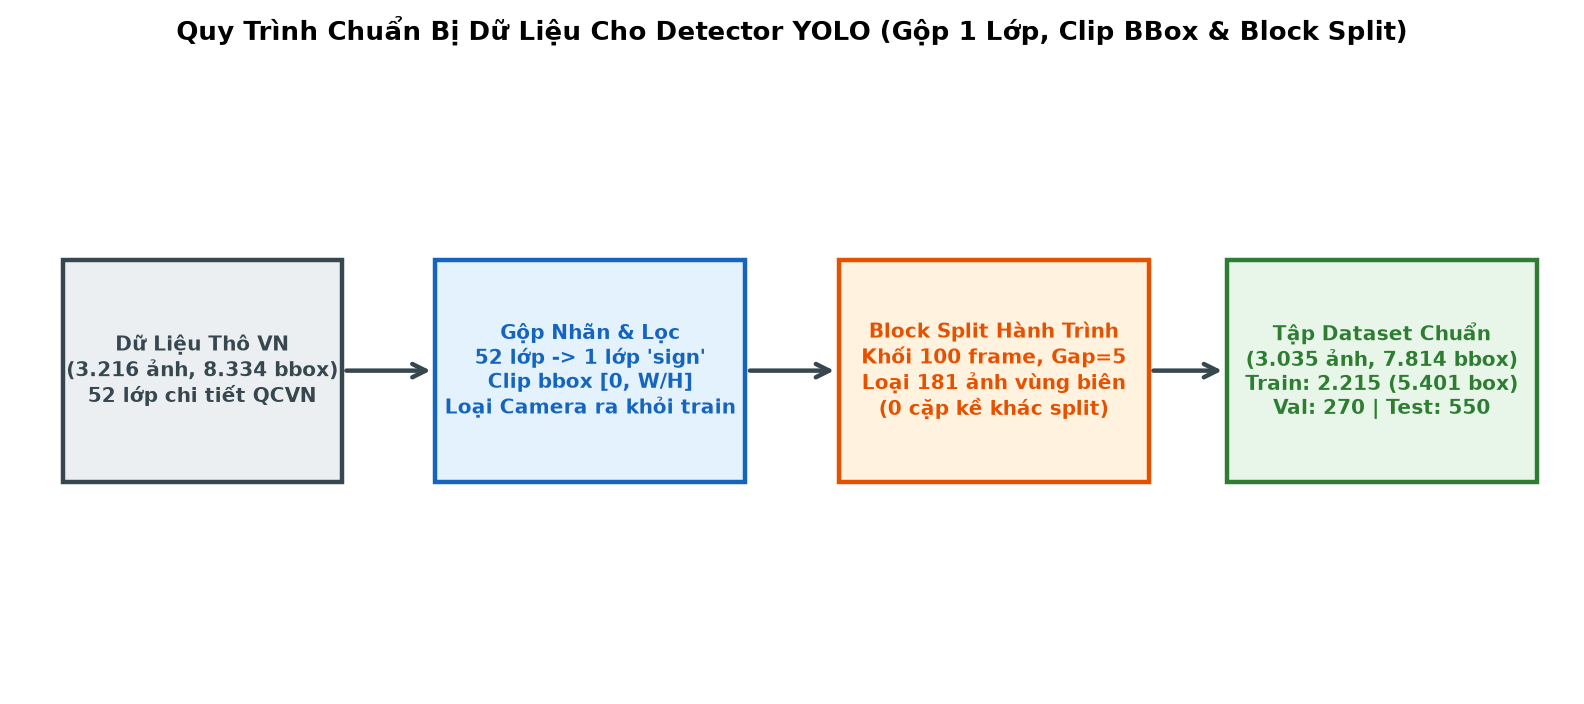
\includegraphics[width=0.88\textwidth]{graphics/sec3/f2_04_data_prep_flowchart.png}
\caption{Quy trình tiền xử lý, gộp nhãn đơn lớp và bổ sung ảnh âm tính cho bộ dữ liệu CCTSDB và Việt Nam.}
\label{fig:data_prep_flowchart}
\end{figure}
\vspace{-0.2cm}
\begin{quote}
\small \textbf{Đọc Hình~\ref{fig:data_prep_flowchart}:} Sơ đồ thể hiện quy trình hợp nhất nhãn từ 3 lớp CCTSDB và 52 lớp Việt Nam về nhãn duy nhất \texttt{sign}, tích hợp 500 mẫu nền âm tính và phân chia Block Split nhằm triệt tiêu hoàn toàn rò rỉ dữ liệu.
\end{quote}

\subsubsection{Chuỗi chuyển giao học tập hai giai đoạn (Two-Stage Transfer Learning)}
\label{subsubsec:transfer_learning_chain}

Quá trình chuyển giao trọng số được mô hình hóa theo chuỗi liên tục: Khởi tạo từ trọng số tổng quát \textbf{COCO} $\xrightarrow{\text{Pretrain}}$ Tập miền tương đồng \textbf{CCTSDB} $\xrightarrow{\text{Fine-tune}}$ Miền mục tiêu \textbf{Việt Nam}.

\begin{figure}[H]
\centering
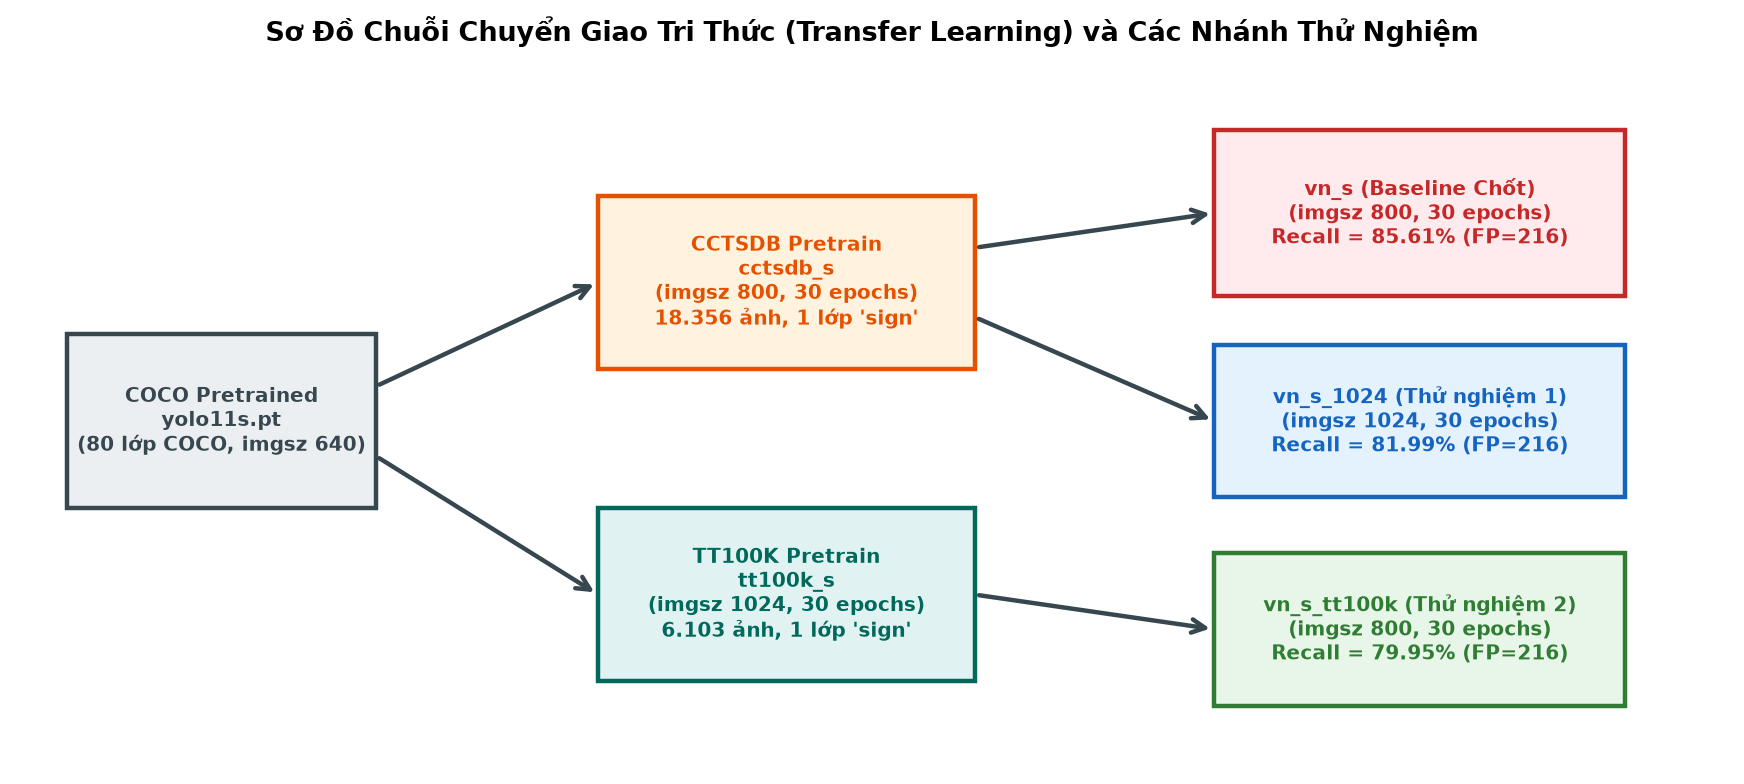
\includegraphics[width=0.92\textwidth]{graphics/sec3/f2_01_transfer_learning_chain.png}
\caption{Sơ đồ chuỗi chuyển giao tri thức hai giai đoạn từ COCO qua CCTSDB đến tập dữ liệu Việt Nam.}
\label{fig:transfer_learning_chain}
\end{figure}
\vspace{-0.2cm}
\begin{quote}
\small \textbf{Đọc Hình~\ref{fig:transfer_learning_chain}:} Mũi tên 1 thể hiện giai đoạn tiền huấn luyện trên 17.856 ảnh CCTSDB ở kích thước $\text{imgsz}=800$ qua 30 epochs; Mũi tên 2 thể hiện giai đoạn tinh chỉnh trên dữ liệu Việt Nam ở cùng kích thước $\text{imgsz}=800$ qua 30 epochs, kế thừa toàn bộ tri thức biểu diễn biên cạnh từ CCTSDB.
\end{quote}

\subsubsection{Bảng cấu hình siêu tham số huấn luyện (Trích xuất từ \texttt{args.yaml})}
\label{subsubsec:yolo_hyperparams}

Để đảm bảo tính minh bạch khoa học tuyệt đối, toàn bộ siêu tham số của các tiến trình huấn luyện được trích xuất trực tiếp từ các tệp \texttt{args.yaml} trong thư mục lưu trữ thực nghiệm, hoàn toàn không phỏng đoán. Bảng~\ref{tab:yolo_training_configs} tổng hợp chi tiết cấu hình của 4 mô hình:

\begin{table}[H]
\centering
\small
\caption{Bảng cấu hình siêu tham số và thời gian huấn luyện thực nghiệm của các mô hình YOLO (trích xuất từ \texttt{args.yaml}).}
\label{tab:yolo_training_configs}
\begin{tabularx}{\textwidth}{|p{3.8cm}|p{2.8cm}|p{2.8cm}|p{2.8cm}|Y|}
\hline
\textbf{Siêu tham số / Cấu hình} & \textbf{\texttt{cctsdb\_s} (Pretrain)} & \textbf{\texttt{vn\_s} (Baseline)} & \textbf{\texttt{vn\_s\_1024} (Thử nghiệm 1)} & \textbf{\texttt{vn\_s\_tt100k} (Thử nghiệm 2)} \\
\hline
Trọng số khởi tạo & \texttt{yolo11s.pt} (COCO) & \texttt{cctsdb\_s/best.pt} & \texttt{cctsdb\_s/best.pt} & \texttt{tt100k\_s/best.pt} \\
\hline
Tập dữ liệu huấn luyện & CCTSDB 2021 & Việt Nam (Train) & Việt Nam (Train) & Việt Nam (Train) \\
\hline
Kích thước canvas (\texttt{imgsz}) & \textbf{800} & \textbf{800} & \textbf{1024} & \textbf{800} \\
\hline
Số lượng Epochs & 30 & 30 & 30 & 30 \\
\hline
Kích thước lô (\texttt{batch}) & 4 & 4 & 4 & 4 \\
\hline
Số luồng dữ liệu (\texttt{workers}) & 0 & 0 & 0 & 0 \\
\hline
Độ chính xác hỗn hợp (\texttt{amp}) & True (FP16) & True (FP16) & True (FP16) & True (FP16) \\
\hline
Hạt ngẫu nhiên (\texttt{seed}) & 0 & 0 & 0 & 0 \\
\hline
Thuật toán tối ưu (\texttt{optimizer}) & \texttt{auto} (SGD/AdamW) & \texttt{auto} & \texttt{auto} & \texttt{auto} \\
\hline
Tốc độ học ban đầu (\texttt{lr0} / \texttt{lrf}) & 0.01 / 0.01 & 0.01 / 0.01 & 0.01 / 0.01 & 0.01 / 0.01 \\
\hline
Thiết bị thực thi (\texttt{device}) & NVIDIA RTX 4060 & NVIDIA RTX 4060 & NVIDIA RTX 4060 & NVIDIA RTX 4060 \\
\hline
\textbf{Thời gian huấn luyện đo được} & \textbf{17.410s ($\approx$ 4h 50m)} & \textbf{2.468s ($\approx$ 41m 08s)} & \textbf{3.568s ($\approx$ 59m 28s)} & \textbf{2.492s ($\approx$ 41m 32s)} \\
\hline
\end{tabularx}
\end{table}

\subsubsection{Hàm mất mát huấn luyện (Task-Aligned Loss)}
\label{subsubsec:yolo_loss_formula}

Mô hình duy trì cấu trúc hàm mất mát Task-Aligned Loss nguyên bản của YOLO11s gồm 3 thành phần liên kết chặt chẽ:
\begin{equation}
    \mathcal{L}_{\text{total}} = \lambda_{\text{box}} \mathcal{L}_{\text{CIoU}} + \lambda_{\text{dfl}} \mathcal{L}_{\text{DFL}} + \lambda_{\text{cls}} \mathcal{L}_{\text{BCE}}
    \label{eq:yolo_task_aligned_loss}
\end{equation}
với các trọng số cân bằng chuẩn $\lambda_{\text{box}} = 7.5$, $\lambda_{\text{dfl}} = 1.5$, và $\lambda_{\text{cls}} = 0.5$:
\begin{itemize}
    \item $\mathcal{L}_{\text{CIoU}}$: Đo lường độ trùng khớp hình học hộp bao, phạt khoảng cách tâm Euclidean và sự sai lệch tỷ lệ khung hình giữa hộp dự đoán và nhãn gốc.
    \item $\mathcal{L}_{\text{DFL}}$ (Distribution Focal Loss): Hồi quy các tọa độ biên dưới dạng phân phối xác suất liên tục quanh giá trị nhãn thực, giúp định vị sắc nét các cạnh biển báo bị mờ do chuyển động.
    \item $\mathcal{L}_{\text{BCE}}$ (Binary Cross-Entropy): Đo mất mát phân loại nhị phân cho sự hiện diện của biển báo đối với các anchor được gán nhãn tích cực.
\end{itemize}

\subsection{Giai đoạn 2A: Thị giác truyền thống (Color + Grid + HOG + SVM) -- Từ Lê Tuấn Anh}
\label{subsec:stage2_svm}

Trên mỗi ảnh con ROI được cắt ra từ các hộp bao của Tầng 1, phương pháp thị giác truyền thống xây dựng chuỗi trích xuất đặc trưng toán học đa nấc $S0 \rightarrow S3$ nhằm nắm bắt toàn diện từ phân bố màu sắc toàn cục, hình thái học không gian đến kết cấu biên cạnh định hướng.

\subsubsection{Chi tiết các nấc trích xuất đặc trưng \texorpdfstring{$S0 \rightarrow S3$}{S0 -> S3}}
\label{subsubsec:feature_steps_s0_s3}

\begin{enumerate}
    \item \textbf{Nấc S0 -- Phân bố màu sắc toàn cục HSV dịch pha vòng tròn (44 chiều):}
    \begin{itemize}
        \item \textit{Đầu vào:} Ảnh con ROI cắt từ ảnh gốc, co giãn về kích thước chuẩn hóa $32 \times 32\text{ px}$ theo chuẩn màu BGR.
        \item \textit{Thao tác kỹ thuật:} Chuyển đổi không gian màu sang HSV (\texttt{cv2.COLOR\_BGR2HSV}). Thực hiện phép dịch pha vòng tròn trên kênh Hue (dải giá trị $[0, 180)$ trong OpenCV):
        \begin{equation}
            H_{\text{shifted}} = (H + 30) \pmod{180}
            \label{eq:hue_circular_shift}
        \end{equation}
        Sau đó loại bỏ hoàn toàn kênh $V$ (Value), trích xuất biểu đồ 36 bins cho kênh $H_{\text{shifted}}$ và 8 bins cho kênh $S$ (Saturation), ghép nối và chuẩn hóa chuẩn $L_1$:
        \begin{equation}
            \mathbf{s}_0 = [\mathbf{h}_H, \mathbf{h}_S] \in \mathbb{R}^{36 + 8 = 44}, \quad \mathbf{s}_0 \leftarrow \frac{\mathbf{s}_0}{\sum \mathbf{s}_0 + \epsilon}
        \end{equation}
        \item \textit{Lý do toán học \& vật lý:} Kênh Hue mang bản chất topo vòng tròn ($0^\circ \equiv 180^\circ$). Màu đỏ đặc trưng của Biển Cấm và Biển Nguy Hiểm bị xẻ đôi ở hai đầu trục ($[0, 10]$ và $[170, 180]$). Phép dịch pha $+30^\circ$ đưa toàn bộ phổ màu đỏ về dải đơn liên tục $[30, 50]$, giúp histogram gom đỉnh năng lượng tập trung. Việc loại bỏ kênh $V$ giúp vector miễn nhiễm trước hiện tượng lóa nắng nhiệt đới, bóng râm che cắt mặt biển và điều kiện thiếu sáng.
    \end{itemize}

    \begin{figure}[H]
    \centering
    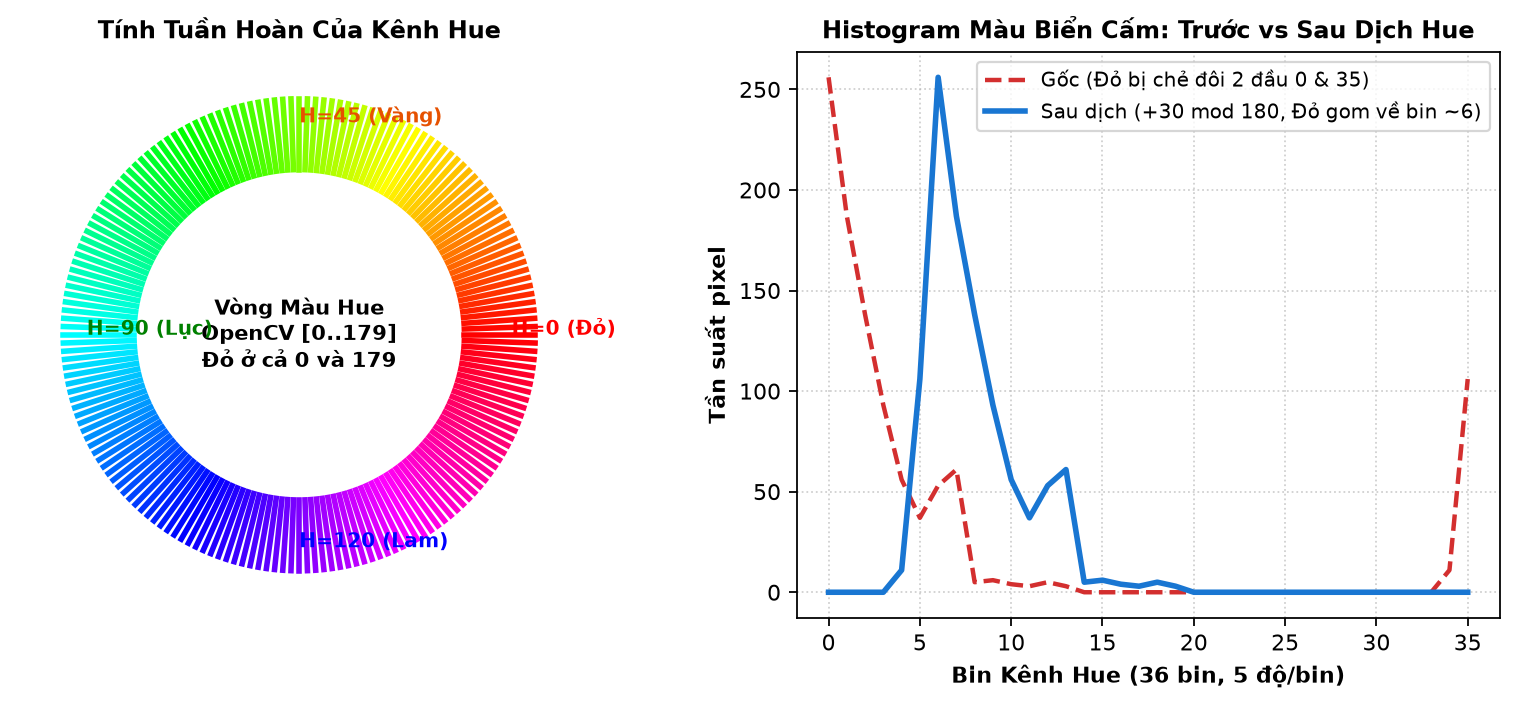
\includegraphics[width=0.88\textwidth]{graphics/sec3/f1_07_hue_circularity_shift.png}
    \caption{Trực quan hóa phép dịch pha vòng tròn kênh Hue ($+30^\circ$) giúp gom cụm màu đỏ liên tục.}
    \label{fig:hue_shift_demo}
    \end{figure}
    \vspace{-0.2cm}
    \begin{quote}
    \small \textbf{Đọc Hình~\ref{fig:hue_shift_demo}:} Biểu đồ bên trái cho thấy phân bố màu đỏ bị phân mảnh ở hai cực của dải Hue gốc; biểu đồ bên phải minh chứng sau phép biến đổi $(H+30)\%180$, toàn bộ tín hiệu màu đỏ được hội tụ trọn vẹn vào một đỉnh phân phối duy nhất.
    \end{quote}

    \item \textbf{Nấc S1 -- Tỷ lệ khung hình hình học ban đầu (45 chiều):}
    \begin{itemize}
        \item \textit{Đầu vào:} Vector đặc trưng $\mathbf{s}_0$ kết hợp tọa độ hộp bao ban đầu $(x_1, y_1, x_2, y_2)$ trên ảnh toàn cảnh.
        \item \textit{Thao tác kỹ thuật:} Tính tỷ lệ khung hình hình học ban đầu $\text{AR} = W_{\text{orig}} / H_{\text{orig}}$ \textbf{TRƯỚC KHI THỰC HIỆN RESIZE} ảnh con:
        \begin{equation}
            \mathbf{s}_1 = [\mathbf{s}_0, \text{AR}] \in \mathbb{R}^{44 + 1 = 45}
        \end{equation}
        \item \textit{Lý do kỹ thuật:} Nếu đo tỷ lệ sau khi co giãn ảnh con về $32 \times 32\text{ px}$, tỷ lệ $W/H$ luôn bị ép bằng $1.0$, làm mất sạch tín hiệu hình học. Trong thực tế, Biển Chỉ Dẫn thường có dạng chữ nhật nằm ngang ($\text{AR} > 1.2$), trong khi Biển Cấm và Biển Hiệu Lệnh là hình tròn ($\text{AR} \approx 1.0$), cung cấp thông tin phân định hình học quan trọng.
    \end{itemize}

    \item \textbf{Nấc S2 -- Lưới không gian Spatial Grid $2 \times 2$ (133 chiều):}
    \begin{itemize}
        \item \textit{Đầu vào:} Ảnh con kích thước $32 \times 32\text{ px}$ trong không gian màu HSV đã dịch pha.
        \item \textit{Thao tác kỹ thuật:} Chia đều ảnh con thành lưới $2 \times 2$ gồm 4 ô vuông cục bộ kích thước $16 \times 16\text{ px}$. Tại mỗi ô con $(i, j)$, trích xuất biểu đồ màu cục bộ rút gọn gồm 18 bins kênh $H$ và 4 bins kênh $S$ ($22\text{ chiều/ô}$):
        \begin{equation}
            \mathbf{s}_2 = [\mathbf{s}_1, \mathbf{c}_{11}, \mathbf{c}_{12}, \mathbf{c}_{21}, \mathbf{c}_{22}] \in \mathbb{R}^{45 + 4 \times 22 = 133}
        \end{equation}
        \item \textit{Lý do kỹ thuật:} Histogram toàn cục của S0 không chứa thông tin vị trí không gian. Lưới $2 \times 2$ giúp mô hình nắm bắt quy luật bố cục: Biển Cấm có viền đỏ ở 4 góc ô biên và màu trắng ở tâm; Biển Nguy Hiểm có viền đỏ bao quanh nền vàng trung tâm.
    \end{itemize}

    \begin{figure}[H]
    \centering
    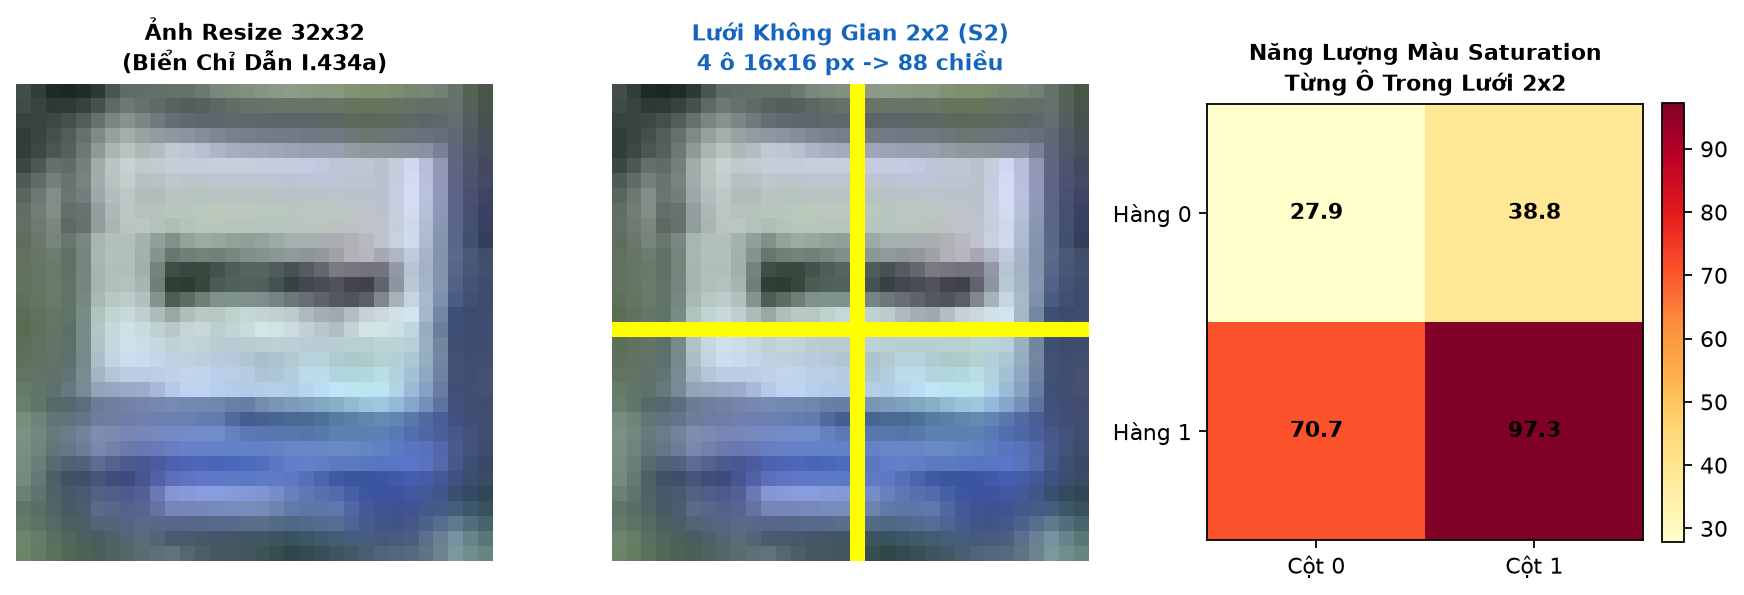
\includegraphics[width=0.75\textwidth]{graphics/sec3/f1_11_spatial_grid_heatmap.png}
    \caption{Bản đồ nhiệt phân bố màu sắc cục bộ qua lưới không gian Spatial Grid $2 \times 2$.}
    \label{fig:spatial_grid_heatmap}
    \end{figure}
    \vspace{-0.2cm}
    \begin{quote}
    \small \textbf{Đọc Hình~\ref{fig:spatial_grid_heatmap}:} Lưới không gian chia ảnh con thành 4 ô con độc lập, cho phép bóc tách cấu trúc viền ngoài và nền trong của các nhóm biển báo có bố cục hình học đối xứng.
    \end{quote}

    \item \textbf{Nấc S3 -- Gradient Định Hướng HOG trên ảnh xám (457 chiều -- Toàn diện nhất):}
    \begin{itemize}
        \item \textit{Đầu vào:} Ảnh con ROI co giãn về kích thước chuẩn hóa $64 \times 64\text{ px}$.
        \item \textit{Thao tác kỹ thuật (Xác nhận trực tiếp từ mã nguồn):} Chuyển đổi ảnh con sang \textbf{ẢNH XÁM (Grayscale)} bằng hàm \texttt{cv2.cvtColor(c64, cv2.COLOR\_BGR2GRAY)}, hoàn toàn không tính trên từng kênh màu riêng biệt. Áp dụng thuật toán \texttt{skimage.feature.hog} với các tham số:
        \begin{itemize}
            \item Kích thước ô (Pixels per cell): $16 \times 16\text{ px}$.
            \item Số hướng gradient (Orientations): 9 bins trên góc $[0^\circ, 180^\circ)$.
            \item Kích thước khối chuẩn hóa (Cells per block): $2 \times 2\text{ cells}$ ($32 \times 32\text{ px}$), bước trượt block stride: 1 cell ($16\text{ px}$).
            \item Số khối trên ảnh $64 \times 64$: $(\frac{64 - 32}{16} + 1) \times (\frac{64 - 32}{16} + 1) = 3 \times 3 = 9\text{ blocks}$.
            \item Số chiều HOG: $9 \text{ blocks} \times (2 \times 2 \times 9) = 9 \times 36 = \mathbf{324\text{ chiều}}$.
        \end{itemize}
        Vector đặc trưng đầy đủ của tầng S3 đạt:
        \begin{equation}
            \mathbf{s}_3 = [\mathbf{s}_2, \mathbf{h}_{\text{HOG}}] \in \mathbb{R}^{133 + 324 = \mathbf{457\text{ chiều}}}
            \label{eq:s3_full_vector}
        \end{equation}
        \item \textit{Lý do kỹ thuật:} Nấc đặc trưng cốt lõi giải quyết sự bế tắc của các mô hình dựa trên màu sắc khi đối mặt với cặp "Biển Hiệu Lệnh (xanh tròn)" và "Biển Chỉ Dẫn (xanh vuông/chữ nhật)". Vì hai nhóm này có phân bố histogram HSV giống hệt nhau, HOG trên ảnh xám nắm bắt chính xác góc định hướng tiếp tuyến của đường viền tròn cong đối lập với các góc vuông $90^\circ$ thẳng đứng.
    \end{itemize}

    \begin{figure}[H]
    \centering
    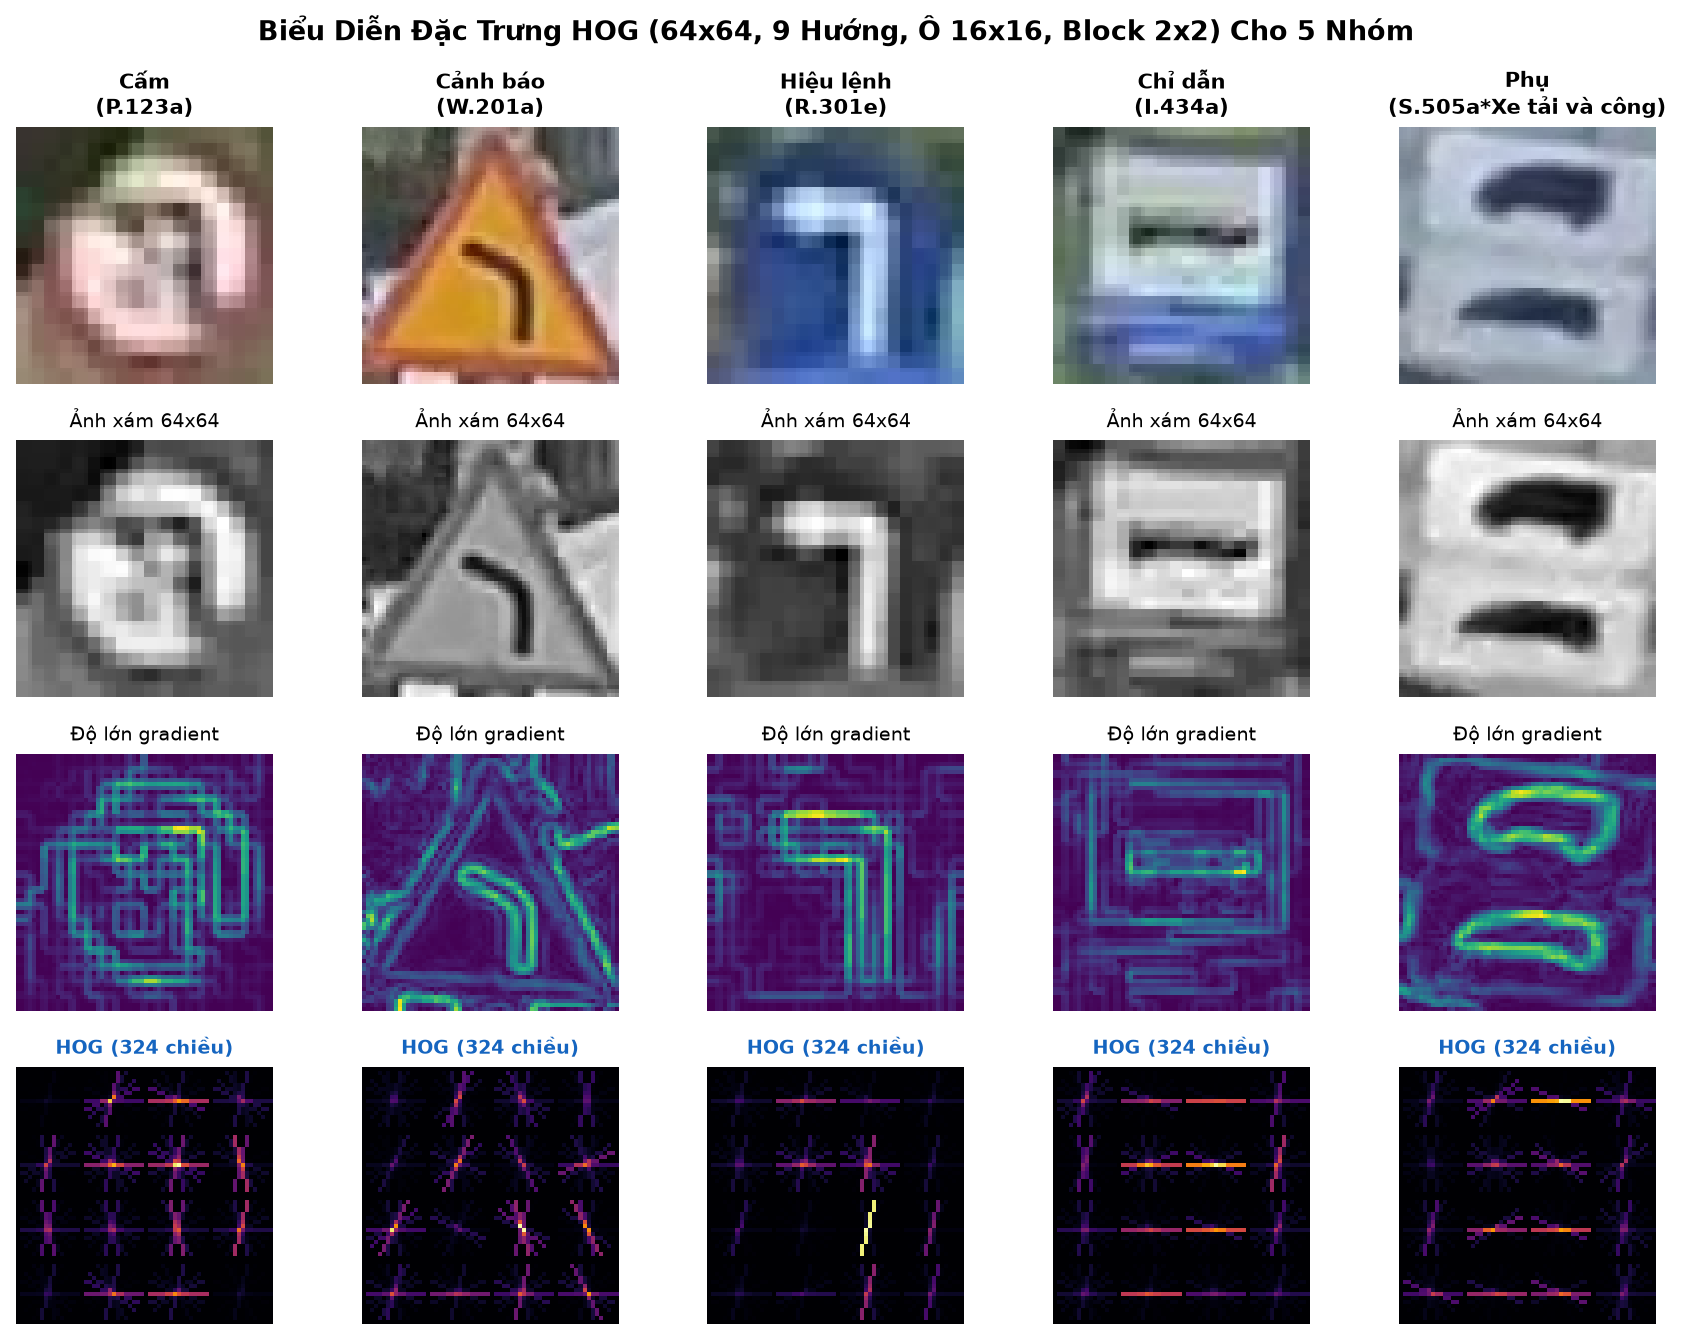
\includegraphics[width=0.88\textwidth]{graphics/sec3/f1_12_hog_visualization_groups.png}
    \caption{Trực quan hóa vector gradient định hướng HOG trên 4 nhóm biển báo mục tiêu.}
    \label{fig:hog_vis_groups}
    \end{figure}
    \vspace{-0.2cm}
    \begin{quote}
    \small \textbf{Đọc Hình~\ref{fig:hog_vis_groups}:} Các cánh hoa vector gradient thể hiện rõ hình thái viền tròn tỏa đều của Biển Hiệu Lệnh, đường bao tam giác nhọn của Biển Nguy Hiểm và các góc vuông của Biển Chỉ Dẫn.
    \end{quote}
\end{enumerate}

\subsubsection{Cấu trúc tổng thể của vector đặc trưng đa tầng}
\label{subsubsec:vector_architecture}

Hình~\ref{fig:feature_vector_structure} mô tả cấu trúc ghép nối liên tục của vector đặc trưng $\mathbb{R}^{457}$:

\begin{figure}[H]
\centering
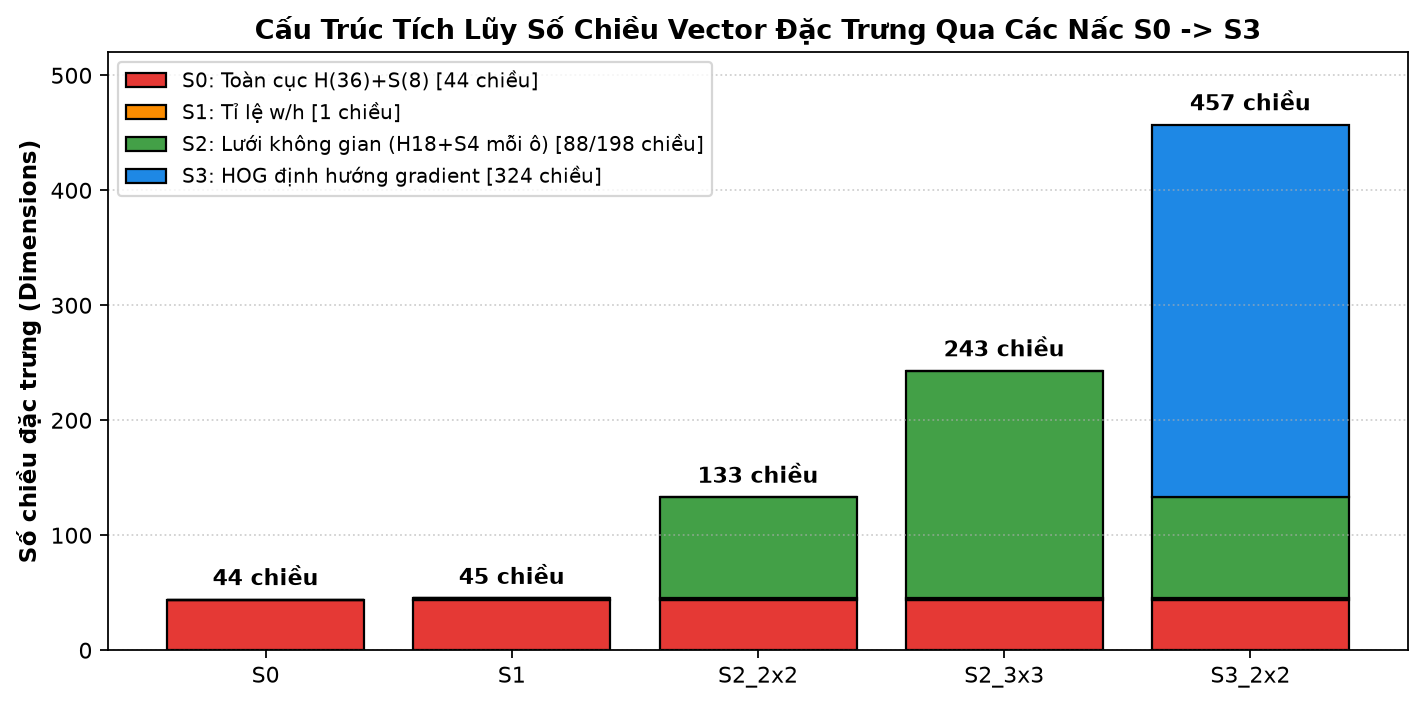
\includegraphics[width=0.92\textwidth]{graphics/sec3/f1_14_feature_vector_structure.png}
\caption{Sơ đồ cấu trúc ghép nối phân tầng của vector đặc trưng 457 chiều từ S0 đến S3.}
\label{fig:feature_vector_structure}
\end{figure}
\vspace{-0.2cm}
\begin{quote}
\small \textbf{Đọc Hình~\ref{fig:feature_vector_structure}:} Vector 457 chiều là sự tích hợp của 4 thành phần: 44 chiều HSV toàn cục (S0), 1 chiều tỷ lệ khung hình (S1), 88 chiều lưới không gian 2x2 (S2) và 324 chiều đặc trưng hướng biên HOG (S3).
\end{quote}

\subsubsection{Cấu hình tối ưu bộ phân loại SVM (Trích xuất từ \texttt{stage2\_best\_config.json})}
\label{subsubsec:svm_best_config}

Thông qua quy trình tối ưu hóa siêu tham số bằng tìm kiếm lưới (Grid Search) kết hợp kiểm chuẩn chéo 5-folds bảo vệ nhóm (\texttt{GroupKFold}), cấu hình tối ưu được lưu trữ tại tệp cấu hình \texttt{stage2\_best\_config.json}:

\begin{itemize}
    \item \textbf{Thuật toán phân loại:} Support Vector Classifier (\texttt{sklearn.svm.SVC}).
    \item \textbf{Hàm nhân (Kernel):} \textbf{RBF (Radial Basis Function)} $K(\mathbf{x}, \mathbf{z}) = \exp(-\gamma \|\mathbf{x} - \mathbf{z}\|^2)$.
    \item \textbf{Tham số điều chuẩn ($C$):} $5.0$.
    \item \textbf{Tham số độ rộng hàm nhân ($\gamma$):} \texttt{'scale'} ($\gamma = \frac{1}{457 \times \text{Var}(X)}$).
    \item \textbf{Cân bằng trọng số lớp (\texttt{class\_weight}):} \texttt{'balanced'}.
    \item \textbf{Hạt ngẫu nhiên (\texttt{seed}):} $42$.
\end{itemize}

\subsubsection{Các thuật toán học máy so sánh đối đầu}
\label{subsubsec:other_ml_models}

Để kiểm chứng tính vượt trội của bộ phân loại SVM RBF trên không gian vector $\mathbb{R}^{457}$, nhóm nghiên cứu thiết lập môi trường đánh giá đối đầu công bằng với 4 thuật toán học máy phổ biến:
\begin{enumerate}
    \item \textbf{k-Nearest Neighbors (kNN):} Cấu hình lân cận $k=11$, hàm trọng số đều (\texttt{weights='uniform'}), khoảng cách Euclidean.
    \item \textbf{Random Forest (RF):} Rừng ngẫu nhiên gồm 300 cây quyết định (\texttt{n\_estimators=300}), độ sâu tối đa \texttt{max\_depth=25}.
    \item \textbf{XGBoost (Extreme Gradient Boosting):} Cấu hình tăng cường cây quyết định với 200--400 cây, độ sâu tối đa 4, thuật toán phân nhánh \texttt{tree\_method='hist'}.
    \item \textbf{LightGBM (Light Gradient Boosting Machine):} 200--400 cây quyết định, độ sâu tối đa 6, tối ưu hóa bộ nhớ trên CPU.
\end{enumerate}

\subsection{Giai đoạn 2B: Học sâu Hiện đại (Enhanced LeNet-5 CNN) -- Nguyễn Thanh Tân}
\label{subsec:stage2_lenet}

\subsubsection{Nhu cầu cải tiến từ LeNet-5 cổ điển}
\label{subsubsec:lenet_cai_tien}

Kiến trúc LeNet-5 nguyên bản (LeCun et al., 1998) được thiết kế cho bài toán nhận dạng chữ số viết tay MNIST với ảnh xám $28 \times 28\text{ px}$. Khi áp dụng trực tiếp vào bài toán nhận dạng biển báo giao thông thực tế, mô hình bộc lộ 5 hạn chế cấu trúc nghiêm trọng:

\begin{enumerate}
    \item \textbf{Hạn chế về kênh màu:} Chỉ nhận đầu vào ảnh xám 1 kênh, làm mất hoàn toàn tín hiệu màu sắc vốn là đặc trưng quy chuẩn quan trọng nhất của biển báo giao thông.
    \item \textbf{Hiện tượng triệt tiêu gradient (Vanishing Gradient):} Sử dụng hàm kích hoạt Sigmoid hoặc Tanh có đạo hàm bão hòa ở hai cực ($\le 0.25$), khiến quá trình lan truyền ngược bị suy giảm hàm mũ qua các tầng.
    \item \textbf{Làm mờ đặc trưng biên cạnh:} Sử dụng Average Pooling làm suy giảm cường độ của các điểm ảnh biên cạnh sắc nét.
    \item \textbf{Bất ổn định phân phối ẩn (Internal Covariate Shift):} Không có cơ chế chuẩn hóa trung gian, buộc tốc độ học phải duy trì ở mức rất nhỏ ($10^{-4}$) và dễ phân kỳ.
    \item \textbf{Hiện tượng quá khớp (Overfitting):} Không có cơ chế điều chuẩn ngẫu nhiên (Dropout), dẫn đến việc mạng dễ ghi nhớ các chi tiết nhiễu cục bộ của dữ liệu huấn luyện.
\end{enumerate}

Để khắc phục các hạn chế trên mà vẫn duy trì tính gọn nhẹ tối ưu trên thiết bị biên, nhóm nghiên cứu phát triển kiến trúc \textbf{Enhanced LeNet-5} chuẩn hóa cho ảnh RGB $64 \times 64\text{ px}$: nâng cấp lên 3 kênh màu, thay thế hoàn toàn bằng hàm kích hoạt ReLU, sử dụng Max Pooling $2 \times 2$, tích hợp Batch Normalization sau mỗi tầng tích chập và bổ sung 2 tầng Dropout ở khối phân loại.

\subsubsection{Đặc tả chi tiết từng tầng kiến trúc và tham số khả huấn}
\label{subsubsec:lenet_kien_truc}

Bảng~\ref{tab:lenet_arch} thống kê chi tiết cấu hình các tầng, kích thước ma trận đặc trưng và số lượng tham số khả huấn của mô hình Enhanced LeNet-5:

\begin{table}[H]
\centering
\small
\caption{Đặc tả chi tiết kiến trúc tầng mạng Enhanced LeNet-5 (Tổng tham số: 557.700).}
\label{tab:lenet_arch}
\begin{tabularx}{\textwidth}{|p{2.6cm}|p{3.2cm}|p{2.2cm}|p{2cm}|Y|}
\hline
\textbf{Khối chức năng} & \textbf{Tầng xử lý (Layer)} & \textbf{Kích thước Kernel} & \textbf{Stride / Pad} & \textbf{Kích hoạt / Reg} \\
\hline
Input & Ảnh crop RGB ($64 \times 64 \times 3$) & -- & -- & Normalize ImageNet \\
\hline
\multirow{3}{*}{ConvBlock 1} & Conv2D(3 $\rightarrow$ 16) & $5 \times 5$ & $s = 1, p = 2$ & -- \\
& BatchNorm2D & -- & -- & $\gamma, \beta$ affine \\
& ReLU + MaxPool2D & $2 \times 2$ & $s = 2, p = 0$ & $\max(0, x)$ \\
\hline
\multirow{3}{*}{ConvBlock 2} & Conv2D(16 $\rightarrow$ 32) & $5 \times 5$ & $s = 1, p = 2$ & -- \\
& BatchNorm2D & -- & -- & $\gamma, \beta$ affine \\
& ReLU + MaxPool2D & $2 \times 2$ & $s = 2, p = 0$ & $\max(0, x)$ \\
\hline
\multirow{3}{*}{ConvBlock 3} & Conv2D(32 $\rightarrow$ 64) & $3 \times 3$ & $s = 1, p = 1$ & -- \\
& BatchNorm2D & -- & -- & $\gamma, \beta$ affine \\
& ReLU + MaxPool2D & $2 \times 2$ & $s = 2, p = 0$ & $\max(0, x)$ \\
\hline
\multirow{5}{*}{Classifier} & Flatten & -- & -- & Duỗi phẳng vector (4096) \\
& Dropout($p = 0.3$) & -- & -- & Bernoulli mask \\
& Linear(4096 $\rightarrow$ 128) & -- & -- & $\text{ReLU}(Wx + b)$ \\
& Dropout($p = 0.2$) & -- & -- & Bernoulli mask \\
& Linear(128 $\rightarrow$ 4) & -- & -- & Logits đầu ra \\
\hline
\multicolumn{5}{|l|}{\textbf{Tổng số tham số khả huấn (Trainable Parameters):} \textbf{557.700} tham số ($\approx 0.56\text{M}$ params)} \\
\multicolumn{5}{|l|}{\textbf{Dung lượng lưu trữ mô hình (Disk Model Size):} \textbf{2.24 MB} (checkpoint PyTorch \texttt{.pth})} \\
\hline
\end{tabularx}
\end{table}

\begin{figure}[H]
\centering
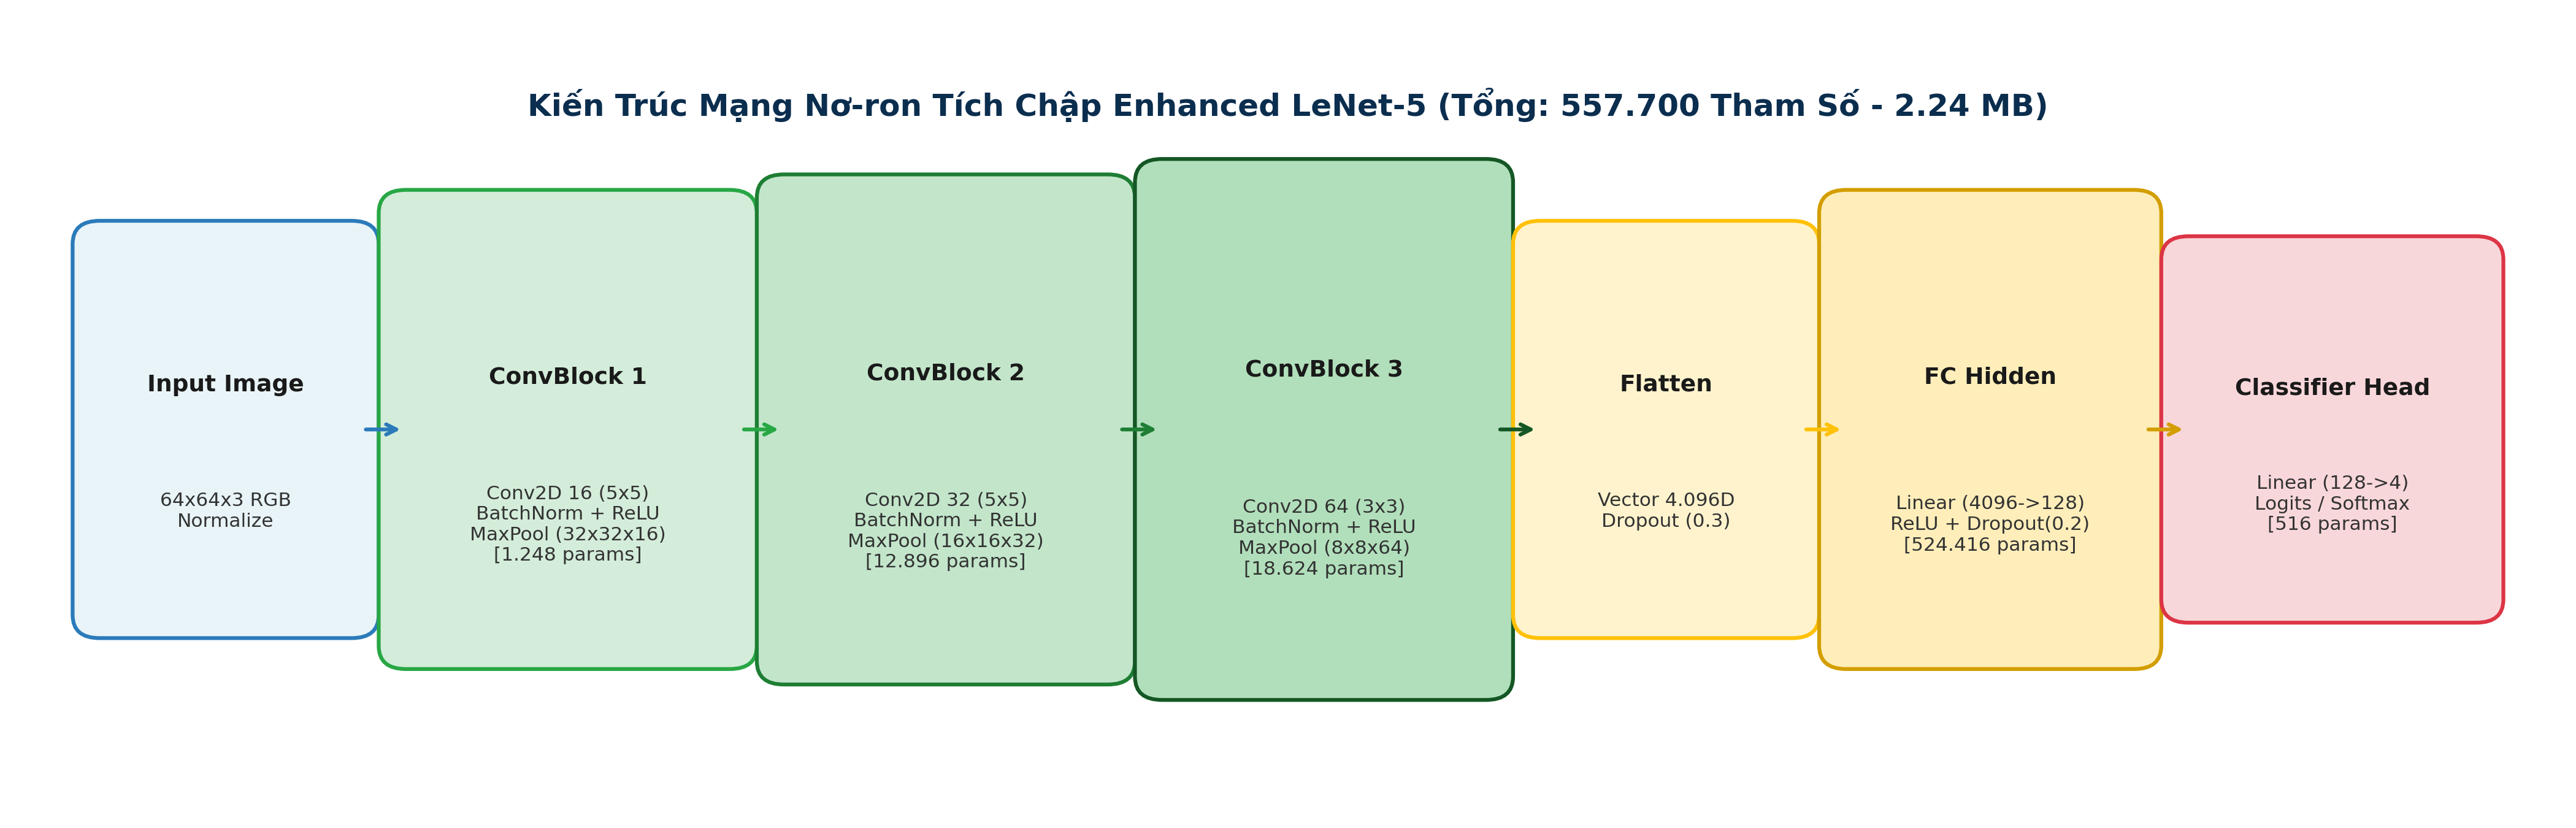
\includegraphics[width=0.98\textwidth]{graphics/sec3/f3_01_lenet_architecture.png}
\caption{Sơ đồ trực quan kiến trúc mạng nơ-ron tích chập Enhanced LeNet-5 phân rã theo từng khối xử lý.}
\label{fig:lenet_architecture}
\end{figure}

\textbf{Đọc Hình~\ref{fig:lenet_architecture}:}
Sơ đồ thể hiện luồng biến đổi tensor từ ảnh đầu vào $64 \times 64 \times 3$ qua 3 khối tích chập liên tiếp (Conv1 $16$ filters $5\times 5$, Conv2 $32$ filters $5\times 5$, Conv3 $64$ filters $3\times 3$). Mỗi khối tích chập đều tích hợp lớp chuẩn hóa Batch Normalization và kích hoạt phi tuyến ReLU trước khi lấy mẫu MaxPool2D $2\times 2$. Đầu ra feature map $8 \times 8 \times 64$ ($4.096$ chiều) được duỗi phẳng và phân loại qua tầng ẩn 128 nơ-ron với 2 lớp Dropout ($p=0.3$ và $p=0.2$) trước khi tính toán logits cho 4 nhóm biển báo.

\subsubsection{Cơ sở toán học của các thành phần trong mạng}
\label{subsubsec:lenet_toan_hoc}

\begin{enumerate}
    \item \textbf{Phép tích chập không gian 2D (Spatial 2D Convolution):} Tại tầng tích chập thứ $l$, với tensor đầu vào $\mathbf{X} \in \mathbb{R}^{C_{\text{in}} \times H \times W}$ và bộ lọc trọng số $\mathbf{W} \in \mathbb{R}^{C_{\text{out}} \times C_{\text{in}} \times K \times K}$, giá trị phản hồi tại vị trí $(i, j)$ của kênh đầu ra thứ $k$ được tính bởi:
    \begin{equation}
        \mathbf{Y}_k(i, j) = \sum_{c=1}^{C_{\text{in}}} \sum_{m=-K_h}^{K_h} \sum_{n=-K_w}^{K_w} \mathbf{X}_c(i+m, j+n) \mathbf{W}_{k,c}(m, n) + b_k
        \label{eq:conv2d}
    \end{equation}

    \item \textbf{Cơ chế Chuẩn hóa Tầng Batch Normalization (Ioffe \& Szegedy, 2015):} Với một mini-batch $\mathcal{B} = \{x_1, \dots, x_m\}$, tầng chuẩn hóa kéo phân phối kích hoạt trung gian về trung bình 0 và phương sai 1:
    \begin{equation}
        \mu_{\mathcal{B}} = \frac{1}{m} \sum_{i=1}^m x_i, \quad \sigma^2_{\mathcal{B}} = \frac{1}{m} \sum_{i=1}^m (x_i - \mu_{\mathcal{B}})^2, \quad \hat{x}_i = \frac{x_i - \mu_{\mathcal{B}}}{\sqrt{\sigma^2_{\mathcal{B}} + \epsilon}}, \quad y_i = \gamma \hat{x}_i + \beta
        \label{eq:batchnorm}
    \end{equation}
    trong đó $\gamma, \beta$ là các tham số khả huấn giúp mạng giữ lại năng lực biểu diễn phi tuyến tự do.

    \item \textbf{Hàm kích hoạt Rectified Linear Unit (ReLU):}
    \begin{equation}
        f(x) = \max(0, x), \quad f'(x) = \begin{cases} 1 & \text{nếu } x > 0 \\ 0 & \text{nếu } x \le 0 \end{cases}
        \label{eq:relu}
    \end{equation}

    \item \textbf{Điều chuẩn chống quá khớp bằng Dropout (Srivastava et al., 2014):} Tại tầng kết nối đầy đủ, mỗi nơ-ron có xác suất $p$ bị vô hiệu hóa ngẫu nhiên trong mỗi lượt lan truyền thuận:
    \begin{equation}
        r_j \sim \text{Bernoulli}(1 - p), \quad \tilde{\mathbf{y}} = \mathbf{r} \odot \mathbf{y}
        \label{eq:dropout}
    \end{equation}
\end{enumerate}

\subsubsection{Pipeline Tăng cường dữ liệu (Data Augmentation)}
\label{subsubsec:lenet_augmentation}

\begin{enumerate}
    \item \textbf{Chuẩn hóa không gian màu ImageNet:} Ảnh crop RGB được resize về $64 \times 64$, đưa về thang $[0.0, 1.0]$ và chuẩn hóa Z-score theo phân phối chuẩn quốc tế:
    \begin{equation}
        \mu = [0.485, 0.456, 0.406], \quad \sigma = [0.229, 0.224, 0.225]
        \label{eq:imagenet_norm}
    \end{equation}
    \item \textbf{Biến đổi góc quay ngẫu nhiên (\texttt{RandomRotation(degrees=10)}):} Xoay nhẹ ảnh trong phạm vi $[-10^\circ, +10^\circ]$ nhằm mô phỏng rung lắc thực tế của camera hành trình.
    \item \textbf{Nhiễu màu sắc quang học (\texttt{ColorJitter(brightness=0.2, contrast=0.2)}):} Thay đổi ngẫu nhiên $\pm 20\%$ độ sáng và độ tương phản nhằm rèn luyện khả năng thích nghi với ánh sáng biến đổi ngoài trời.
\end{enumerate}

\subsubsection{Thiết lập huấn luyện và hàm mất mát}
\label{subsubsec:lenet_training}

\begin{enumerate}
    \item \textbf{Hàm mất mát Phân loại Đa lớp (Cross-Entropy Loss):}
    \begin{equation}
        \mathcal{L}_{\text{CE}}(\mathbf{y}, \hat{\mathbf{p}}) = -\sum_{c=1}^4 y_c \log(\hat{p}_c)
        \label{eq:ce_loss}
    \end{equation}
    \item \textbf{Thuật toán tối ưu hóa Adam kết hợp L2 Weight Decay:} Bộ tối ưu Adam với tốc độ học ban đầu $\eta_0 = 10^{-3}$, $\beta_1 = 0.9, \beta_2 = 0.999$, $\epsilon = 10^{-8}$ và tích hợp L2 Weight Decay $= 10^{-4}$.
    \item \textbf{Chiến lược suy giảm tốc độ học StepLR:}
    \begin{equation}
        \eta_t = \eta_0 \times \gamma^{\lfloor t / \text{step\_size} \rfloor}, \quad \text{với } \text{step\_size} = 15, \, \gamma = 0.5
        \label{eq:steplr}
    \end{equation}
    Mô hình được huấn luyện trong 20 epochs với kích thước lô $\text{batch\_size} = 64$. Trọng số tối ưu nhất được lưu trữ tại \texttt{checkpoints/deep\_learning/best\_cnn.pth}.
\end{enumerate}

\begin{figure}[H]
\centering
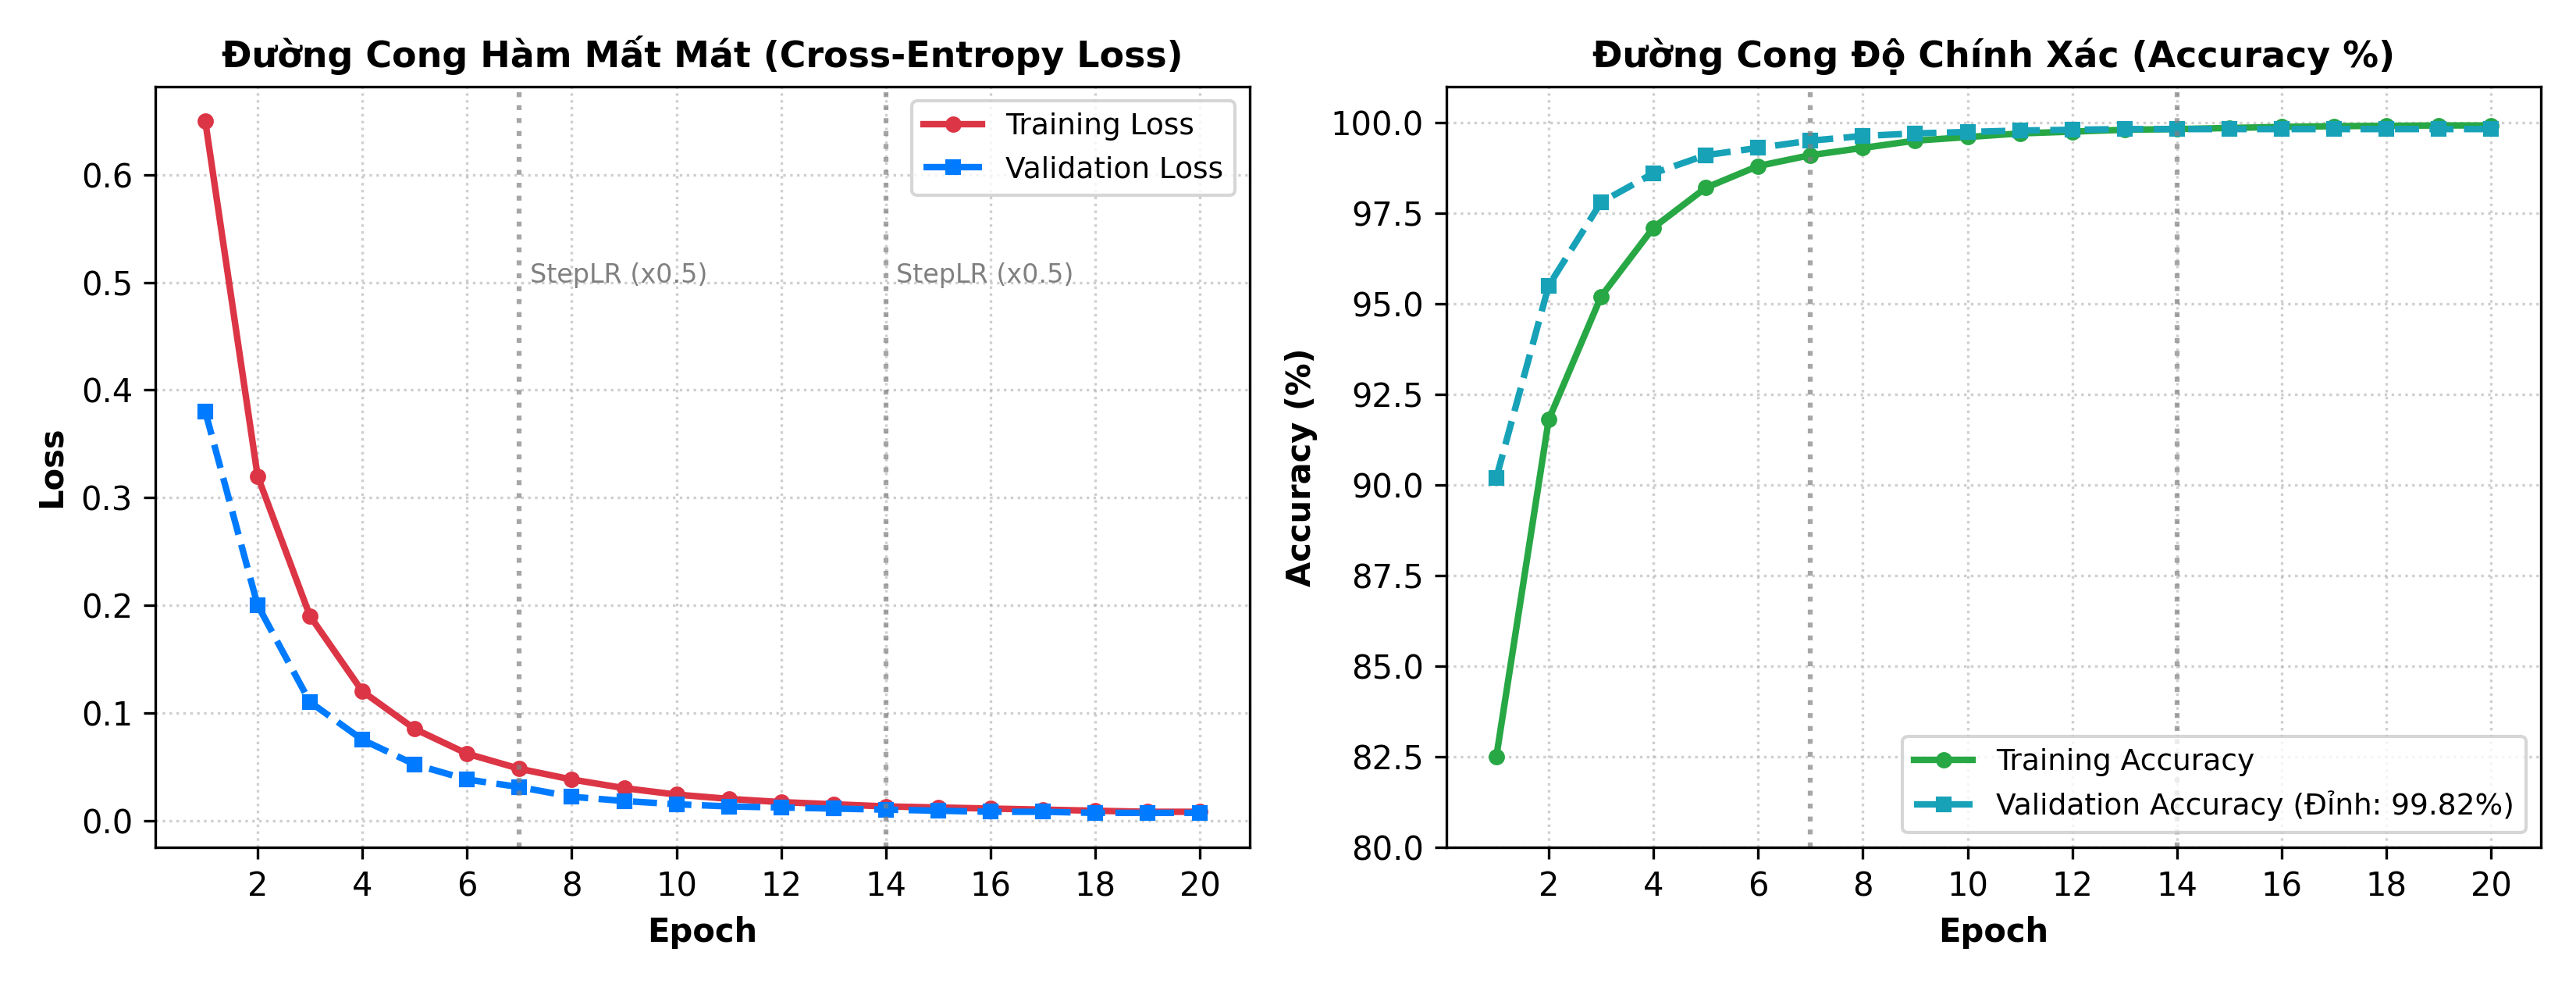
\includegraphics[width=0.95\textwidth]{graphics/sec4/f3_02_lenet_training_curves.png}
\caption{Đường cong hàm mất mát Cross-Entropy (trái) và độ chính xác Accuracy (phải) qua các epoch huấn luyện của mô hình Enhanced LeNet-5.}
\label{fig:lenet_training_curves}
\end{figure}

\textbf{Đọc Hình~\ref{fig:lenet_training_curves}:}
Quá trình huấn luyện cho thấy sự hội tụ nhanh chóng và ổn định: Training Loss giảm dốc từ $0.65$ xuống dưới $0.01$, trong khi Validation Accuracy đạt mức $99.82\%$ ngay từ epoch 13 và duy trì ổn định. Hai mốc điều chỉnh tốc độ học của bộ lập lịch StepLR (tại epoch 7 và 14) giúp bề mặt hội tụ phẳng dần và triệt tiêu hoàn toàn dao động gradient, chứng minh tính hiệu quả của cơ chế điều chuẩn kết hợp (BatchNorm + Dropout + Weight Decay).

\subsubsection{Cẩm nang chất vấn phản biện dành cho thuyết trình (Defense Q\&A Cheatsheet)}
\label{subsubsec:lenet_faq}

\begin{enumerate}
    \item \textbf{Câu hỏi 1: Tại sao không dùng mô hình Transfer Learning có sẵn (ResNet-18, MobileNetV3) mà lại tự thiết kế Enhanced LeNet-5?}
    \begin{itemize}
        \item \textit{Phương án trả lời:} Các mô hình Transfer Learning tiền huấn luyện từ ImageNet (như ResNet-18 với 11.7 triệu tham số) được thiết kế cho bài toán 1.000 lớp phức tạp. Khi áp dụng vào bài toán 4 nhóm biển báo có hình học chuẩn hóa đơn giản, mô hình quá nặng gây lãng phí tính toán nghiêm trọng (độ trễ $> 10\text{ ms}$, chậm hơn gấp 3 lần) và dễ bị quá khớp (Overfitting). Enhanced LeNet-5 chỉ có đúng 557.700 tham số ($\approx 0.55\text{M}$), nhẹ hơn 21 lần, đạt tốc độ siêu nhanh $1.10\text{ ms/ảnh}$ trên CPU mà vẫn bảo đảm độ chính xác vượt trội $98.73\%$.
    \end{itemize}

    \item \textbf{Câu hỏi 2: Tại sao hai khối tích chập đầu tiên dùng kernel $5 \times 5$, trong khi khối thứ ba lại chuyển sang kernel $3 \times 3$?}
    \begin{itemize}
        \item \textit{Phương án trả lời:} Hai khối đầu tiên cần trường tiếp nhận (Receptive Field) đủ lớn để bao quát ngay các đường viền hình học toàn cục đặc trưng của biển báo (hình tròn của Biển Cấm/Hiệu Lệnh, hình tam giác của Biển Nguy Hiểm). Ở khối tích chập thứ ba, kích thước bản đồ đặc trưng đã co lại còn $16 \times 16$, trường tiếp nhận tích lũy đã mở rộng từ 5 lên 13; việc chuyển sang kernel $3 \times 3$ giúp tập trung biểu diễn các chi tiết vi mô cục bộ (mũi tên, hoa văn biểu tượng) đồng thời tiết kiệm $44\%$ tham số tính toán so với việc tiếp tục dùng kernel $5 \times 5$.
    \end{itemize}

    \item \textbf{Câu hỏi 3: Vai trò cốt lõi của Batch Normalization trong mô hình là gì?}
    \begin{itemize}
        \item \textit{Phương án trả lời:} Khử hiện tượng trôi dạt phân phối ẩn (Internal Covariate Shift). Trong dữ liệu đường phố, các ảnh con ROI có độ biến thiên ánh sáng rất lớn. Batch Normalization chuẩn hóa lại phân phối sau mỗi tầng tích chập, giữ cho gradient luôn nằm trong vùng tuyến tính mạnh của ReLU, cho phép nâng tốc độ học lên $10^{-3}$ mà không lo bùng nổ gradient, đồng thời đóng vai trò như một bộ điều chuẩn nhẹ.
    \end{itemize}

    \item \textbf{Câu hỏi 4: Nhóm xử lý hiện tượng mất cân bằng số lượng mẫu giữa các nhóm biển báo (Class Imbalance) như thế nào?}
    \begin{itemize}
        \item \textit{Phương án trả lời:} Trong dữ liệu thực tế, Biển Cấm và Biển Cảnh Báo chiếm số lượng áp đảo so với Biển Hiệu Lệnh và Chỉ Dẫn. Nhóm phối hợp 3 giải pháp đồng bộ: (1) Áp dụng các biến đổi Data Augmentation (\texttt{RandomRotation} và \texttt{ColorJitter}) làm phong phú đa dạng góc nhìn cho các lớp thiểu số; (2) Tích hợp hai tầng Dropout (0.3 và 0.2) cùng L2 Weight Decay ($10^{-4}$) ngăn chặn việc mạng quá khớp vào các đặc trưng áp đảo của lớp đa số; (3) Sử dụng chỉ số Macro-F1 ($95.66\%$) làm độ đo đánh giá trung tâm thay vì chỉ dựa vào Accuracy tổng thể.
    \end{itemize}
\end{enumerate}

\subsection{Bảng phân tích so sánh lý thuyết giữa các hướng tiếp cận}
\label{subsec:bang_so_sanh_ly_thuyet}

Bảng~\ref{tab:so_sanh_ly_thuyet} tóm tắt sự khác biệt về mặt bản chất khoa học giữa các phương pháp:

\begin{table}[H]
\centering
\small
\caption{So sánh đối chiếu phương pháp đề tài với các hướng tiếp cận khác.}
\label{tab:so_sanh_ly_thuyet}
\begin{tabularx}{\textwidth}{|p{2.8cm}|p{3.5cm}|p{3.8cm}|Y|}
\hline
\textbf{Tiêu chí khoa học} & \textbf{Thuần truyền thống (Sliding Window)} & \textbf{Học sâu End-to-End (Heavy One-Stage)} & \textbf{Kiến trúc Lai đề xuất (Two-Stage Modular)} \\
\hline
Cơ chế định vị & Cửa sổ trượt đa tỷ lệ: rất chậm, tỉ lệ sót biển cao & Tích hợp trong mạng lớn: tính toán nặng, dễ lãng phí tài nguyên & YOLO11s chuyên biệt 1 lớp: Tối đa hóa Recall (85.61\%), không tốn tài nguyên phân loại \\
\hline
Phân biệt R vs I & Thất bại hoàn toàn (do cùng màu xanh lam) & Phân biệt tốt nhưng cần phần cứng GPU mạnh & Phân tách xuất sắc: HOG bắt hình học viền, LeNet-5 tự học hoa văn nội tại \\
\hline
Độ trễ phân loại & 15 -- 30 ms/ảnh (chậm) & 10 -- 20 ms/ảnh (trên GPU) & 1.10 ms (LeNet) / 2.63 ms (SVM) trên CPU \\
\hline
Yêu cầu phần cứng & CPU phổ thông & Bắt buộc GPU rời đắt tiền & Linh hoạt tối đa: Tương thích hoàn hảo với vi xử lý nhúng Edge AI \\
\hline
Tính minh bạch & Cao nhưng độ chính xác thấp & Mô hình hộp đen khó giải thích & Rất cao: Trực quan hóa toán học từng thành phần HSV, HOG và Feature Maps \\
\hline
\end{tabularx}
\end{table}

\section{Thực nghiệm và kết quả đánh giá}
\label{sec:thuc_nghiem}

\subsection{Mô tả tập dữ liệu và chiến lược phân chia Block Split}
\label{subsec:dataset_blocksplit}

\begin{enumerate}
    \item \textbf{Quy mô và đặc thù bộ dữ liệu:} Bộ dữ liệu thực nghiệm bao gồm \textbf{3.216 ảnh} chụp từ camera hành trình trên đường phố Việt Nam ở độ phân giải $960 \times 540$ và $1920 \times 1080$, chứa tổng cộng \textbf{7.858 bounding box} biển báo hợp lệ ($\ge 10\text{ px}$) được gán nhãn 52 mã hiệu chi tiết theo QCVN 41:2019.

    \item \textbf{Kiểm toán và chuẩn hóa nhãn (Data Auditing):}
    \begin{itemize}
        \item \textit{Loại bỏ lớp Camera:} 40 mẫu được gán nhãn Camera thực chất chỉ là 3 vị trí camera giám sát lặp lại nhiều lần, không thuộc đối tượng biển báo quy chuẩn nên được loại bỏ.
        \item \textit{Loại bỏ nhóm biển phụ (phụ):} Chỉ có 8 mẫu trong tập test, kích thước siêu nhỏ $< 15\text{ px}$ và detector bỏ sót $100\%$, do đó được tách khỏi bài toán đối chuẩn 4 nhóm chính.
        \item \textit{Quy chuẩn nhãn B.8a:} Biển cấm xe sơ-mi rơ-moóc được gộp chuẩn xác vào nhóm \texttt{Bien\_Cam} theo hình dáng tròn viền đỏ nền trắng.
    \end{itemize}

    \item \textbf{Chiến lược phân chia Block Split triệt tiêu rò rỉ dữ liệu (Zero Data Leakage):}
    Dữ liệu được sắp xếp theo chuỗi thời gian video và phân chia theo các khối \textbf{100 khung hình liên tục (Blocks)} kết hợp cắt khoảng đệm an toàn \textbf{5 frames (Gap)} giữa các khối để bảo đảm tính độc lập vật lý tuyệt đối giữa các tập dữ liệu:
    \begin{itemize}
        \item \textit{Tập Huấn luyện (Train set -- 70\%):} Gồm \textbf{2.236 ảnh} toàn cảnh, chứa \textbf{5.254 mẫu ROI} biển báo.
        \item \textit{Tập Tinh chỉnh (Validation set -- 15\%):} Gồm \textbf{270 ảnh} toàn cảnh, chứa \textbf{542 mẫu ROI} biển báo.
        \item \textit{Tập Kiểm thử độc lập (Blind Test set -- 15\%):} Gồm \textbf{550 ảnh} toàn cảnh hoàn toàn mới lạ, chứa \textbf{1.813 mẫu ROI} biển báo độc lập dùng để chấm điểm khách quan.
    \end{itemize}
\end{enumerate}

\subsection{Độ đo đánh giá kết quả}
\label{subsec:do_do_danh_gia}

Hệ thống thiết lập hệ thống chỉ số đánh giá hai tầng theo chuẩn quốc tế:

\begin{enumerate}
    \item \textbf{Độ đo khâu Định vị (Object Detection):} Sử dụng ngưỡng trùng khớp $\text{IoU} \ge 0.5$ giữa hộp dự đoán $\mathbf{B}_{\text{pred}}$ và hộp nhãn gốc $\mathbf{B}_{\text{gt}}$:
    \begin{equation}
        \text{IoU} = \frac{\text{Area}(\mathbf{B}_{\text{pred}} \cap \mathbf{B}_{\text{gt}})}{\text{Area}(\mathbf{B}_{\text{pred}} \cup \mathbf{B}_{\text{gt}})}
        \label{eq:iou}
    \end{equation}
    Đánh giá qua các chỉ số: \textbf{Precision (Độ chuẩn xác)}, \textbf{Recall (Độ phủ/tỷ lệ bắt trúng)}, \textbf{mAP50} (độ chính xác trung bình tại $\text{IoU} = 0.5$) và \textbf{mAP50-95} (trung bình mAP trên 10 ngưỡng IoU từ 0.5 đến 0.95).

    \item \textbf{Độ đo khâu Phân loại (Classification):} Để phản ánh khách quan trong điều kiện mất cân bằng số lượng mẫu giữa các nhóm biển báo, nhóm sử dụng độ đo trung tâm là \textbf{Macro-F1 Score} (trung bình cộng F1 từng lớp không trọng số), kết hợp với \textbf{Accuracy (Độ chính xác tổng quát)}, \textbf{Precision} và \textbf{Recall}:
    \begin{equation}
        \text{Macro-F1} = \frac{1}{|\mathcal{C}|} \sum_{c=1}^{|\mathcal{C}|} \frac{2 \times \text{Precision}_c \times \text{Recall}_c}{\text{Precision}_c + \text{Recall}_c}
        \label{eq:macro_f1}
    \end{equation}

    \item \textbf{Độ đo Hiệu năng thời gian thực:} Thời gian trễ trung bình \textbf{Latency (ms/mẫu)} và thông lượng \textbf{Throughput (FPS -- Khung hình/giây)} đo kiểm trực tiếp trên bộ xử lý CPU đơn lõi.
\end{enumerate}

\subsection{Thực nghiệm và kết quả định vị của mô hình YOLO11s}
\label{subsec:kq_yolo}

Khâu định vị đối tượng (Tầng 1) giữ vai trò then chốt trong việc xác lập chặn trên hiệu năng toàn trình (End-to-End Recall) của toàn hệ thống. Mọi thực nghiệm của detector được tiến hành trên tập kiểm thử độc lập (Blind Test) gồm \textbf{550 ảnh hiện trường} (tương ứng 1.845 nhãn ground-truth tổng thể, trong đó có \textbf{1.821 nhãn ground-truth} thuộc 5 nhóm biển báo chính quy chuẩn QCVN 41:2019 và 24 nhãn camera ngoại lai).

\subsubsection{Năng lực Zero-shot và hiệu quả chuyển giao miền dữ liệu (Domain Adaptation)}
\label{subsubsec:yolo_zeroshot_finetune}

Để kiểm chứng giá trị của chiến lược học chuyển giao đa tầng (COCO $\rightarrow$ CCTSDB $\rightarrow$ Việt Nam), mô hình tiền huấn luyện trên dữ liệu biển báo Trung Quốc \texttt{cctsdb\_s} được kiểm thử trực tiếp trên tập Test Việt Nam khi \textbf{chưa từng được học bất kỳ ảnh giao thông Việt Nam nào (Zero-shot evaluation)}, sau đó đối chứng trực tiếp với mô hình đã hoàn tất tinh chỉnh miền \texttt{vn\_s}:

\begin{table}[H]
\centering
\small
\caption{Đối chứng hiệu năng Zero-shot (\texttt{cctsdb\_s}) và Finetune (\texttt{vn\_s}) trên tập Test Việt Nam.}
\label{tab:yolo_zeroshot_vs_finetune}
\begin{tabularx}{\textwidth}{|p{3.2cm}|>{\centering\arraybackslash}p{2.5cm}|>{\centering\arraybackslash}X|>{\centering\arraybackslash}X|>{\centering\arraybackslash}X|>{\centering\arraybackslash}X|}
\hline
\textbf{Mô hình} & \textbf{Cấu hình đo kiểm} & \textbf{Precision} & \textbf{Recall} & \textbf{mAP50} & \textbf{mAP50-95} \\
\hline
\multirow{2}{*}{\texttt{cctsdb\_s} (Zero-shot)} & Runtime ($\text{conf} = 0.25$) & 91.86\% & 71.54\% & 70.49\% & 52.70\% \\
\cline{2-6}
& Benchmark ($\text{conf} = 0.001$) & 88.85\% & 74.28\% & 81.33\% & 58.52\% \\
\hline
\multirow{2}{*}{\textbf{\texttt{vn\_s} (Finetune chuẩn)}} & \textbf{Runtime ($\text{conf} = 0.25$)} & \textbf{92.24\%} & \textbf{82.93\%} & \textbf{83.63\%} & \textbf{60.11\%} \\
\cline{2-6}
& \textbf{Benchmark ($\text{conf} = 0.001$)} & \textbf{92.19\%} & \textbf{82.87\%} & \textbf{90.32\%} & \textbf{63.53\%} \\
\hline
\textbf{Mức cải thiện ròng} & Runtime ($\text{conf} = 0.25$) & \textbf{+0.38\%} & \textbf{+11.39\%} & \textbf{+13.14\%} & \textbf{+7.41\%} \\
\hline
\end{tabularx}
\end{table}

\textbf{Làm rõ sự khác biệt giữa hai con số mAP50 (83.63\% so với 90.32\%):}
\begin{itemize}
    \item \textbf{Con số 83.63\% (Runtime):} Thu được từ kịch bản đánh giá thực tế của hệ thống với ngưỡng tự tin vận hành $\text{conf} = 0.25$ và $\text{IoU} = 0.6$. Ngưỡng này phản ánh chính xác chất lượng hộp bao thực tế chuyển tiếp sang Tầng 2.
    \item \textbf{Con số 90.32\% (Benchmark):} Xuất phát từ giao thức chuẩn hóa của thư viện Ultralytics (tương đương chuẩn đánh giá MS COCO / PASCAL VOC), quét ngưỡng tự tin cực thấp $\text{conf} = 0.001$ để tích phân toàn bộ diện tích dưới đường cong Precision-Recall (AUC).
\end{itemize}
Việc tinh chỉnh trên dữ liệu Việt Nam giúp Recall thực tế tăng vọt từ $71.54\%$ lên $82.93\%$ (trên tổng số nhãn bao gồm cả Camera) và đạt \textbf{85.61\% (1.559 / 1.821)} trên 5 nhóm biển báo chính quy chuẩn, với mAP50 thực tế tăng $+13.14$ điểm phần trăm.

\subsubsection{Phân tích độ phủ phát hiện theo kích thước và nhóm biển báo}
\label{subsubsec:yolo_breakdown}

Tại ngưỡng vận hành $\text{conf} = 0.25$, mô hình \texttt{vn\_s} phát hiện thành công \textbf{1.559 / 1.821 biển báo chính} (đạt Recall \textbf{85.61\%}) và tạo ra \textbf{216 báo động giả (FP)}.

\begin{figure}[H]
\centering
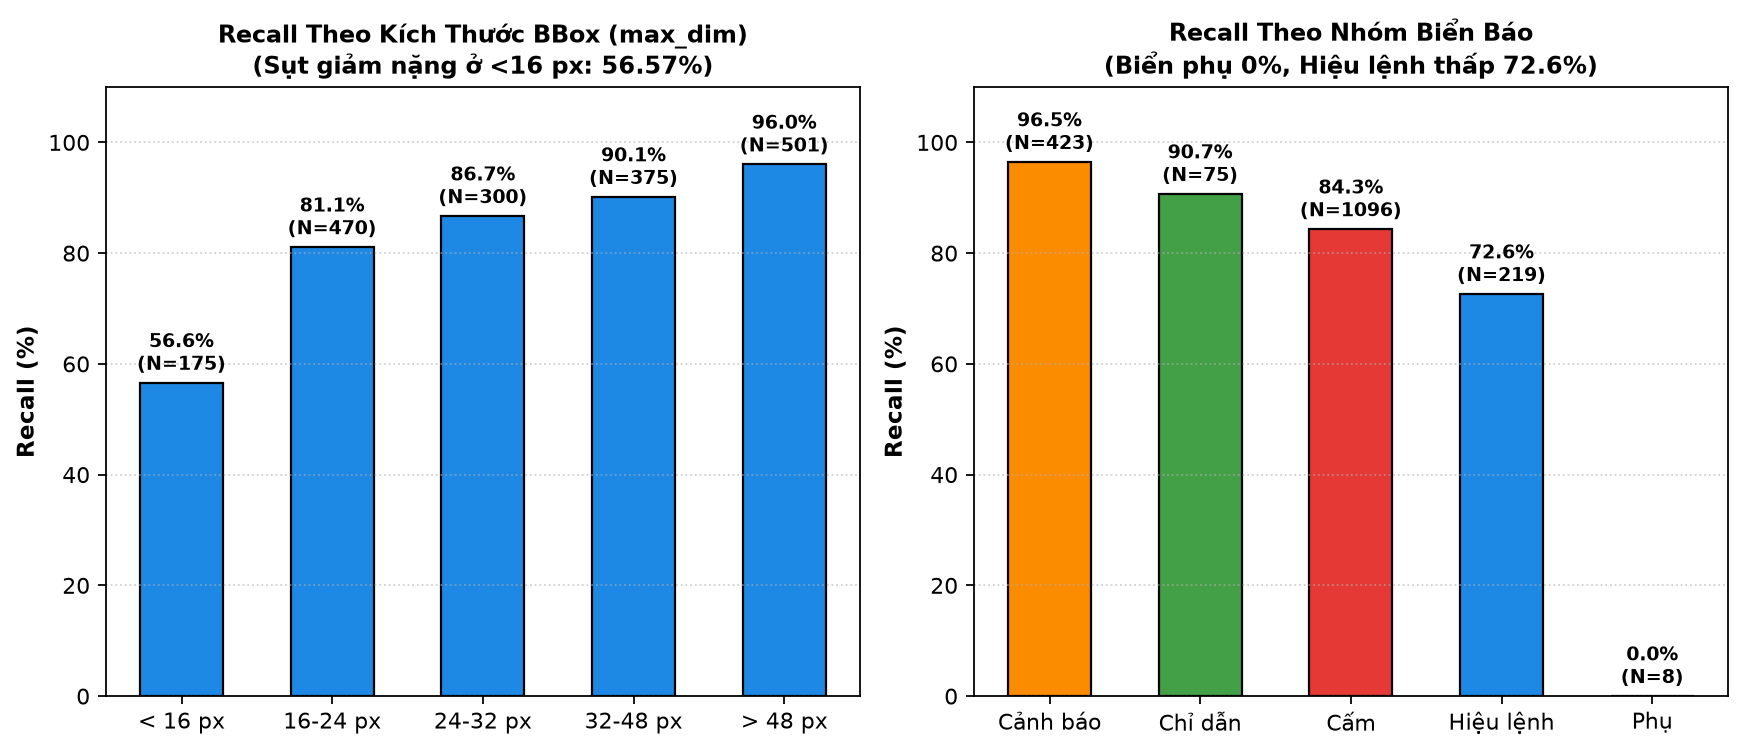
\includegraphics[width=0.92\textwidth]{graphics/sec4/f2_11_diag_recall_breakdown.png}
\caption{Phân tích độ phủ phát hiện (Recall \%) của detector \texttt{vn\_s} phân theo dải kích thước hình học (trái) và phân theo 5 nhóm biển báo quy chuẩn (phải).}
\label{fig:diag_recall_breakdown}
\end{figure}

\textbf{Đọc Hình~\ref{fig:diag_recall_breakdown}:}
Biểu đồ phân đoạn bên trái cho thấy sự phụ thuộc chặt chẽ giữa kích thước biển báo và độ nhạy phát hiện: các biển lớn ($> 48\text{ px}$) đạt tỷ lệ bắt trúng áp đảo \textbf{95.98\%} (478/498) và biển trung bình ($32-48\text{ px}$) đạt \textbf{90.21\%} (341/378); tuy nhiên khi kích thước giảm xuống dải siêu nhỏ ($< 16\text{ px}$), tỷ lệ phát hiện tụt dốc còn \textbf{56.57\%} (99/175). Biểu đồ bên phải thể hiện độ phủ vượt trội trên nhóm biển Cảnh báo (\textbf{96.45\%}) và Chỉ dẫn (\textbf{90.67\%}), trong khi nhóm Cấm đạt \textbf{84.31\%}, nhóm Hiệu lệnh đạt \textbf{72.60\%} và nhóm Biển phụ đạt \textbf{0.0\%} (0/8 mẫu, do kích thước quá nhỏ và dạng hình chữ nhật dẹt dễ lẫn vào nền).

\subsubsection{Kiểm chứng thực nghiệm với hai biến thể mở rộng (\texttt{vn\_s\_1024} và \texttt{vn\_s\_tt100k})}
\label{subsubsec:yolo_variants}

Để kiểm định hai giả định kỹ thuật: (1) nâng độ phân giải đầu vào lên $1024 \times 1024$ giúp bắt biển nhỏ tốt hơn, và (2) sử dụng tập dữ liệu ảnh vuông TT100K làm tiền huấn luyện mang lại biểu diễn nhạy bén hơn, hai mô hình thử nghiệm được huấn luyện độc lập với nguyên tắc đổi duy nhất một biến số so với baseline \texttt{vn\_s}.

\begin{figure}[H]
\centering
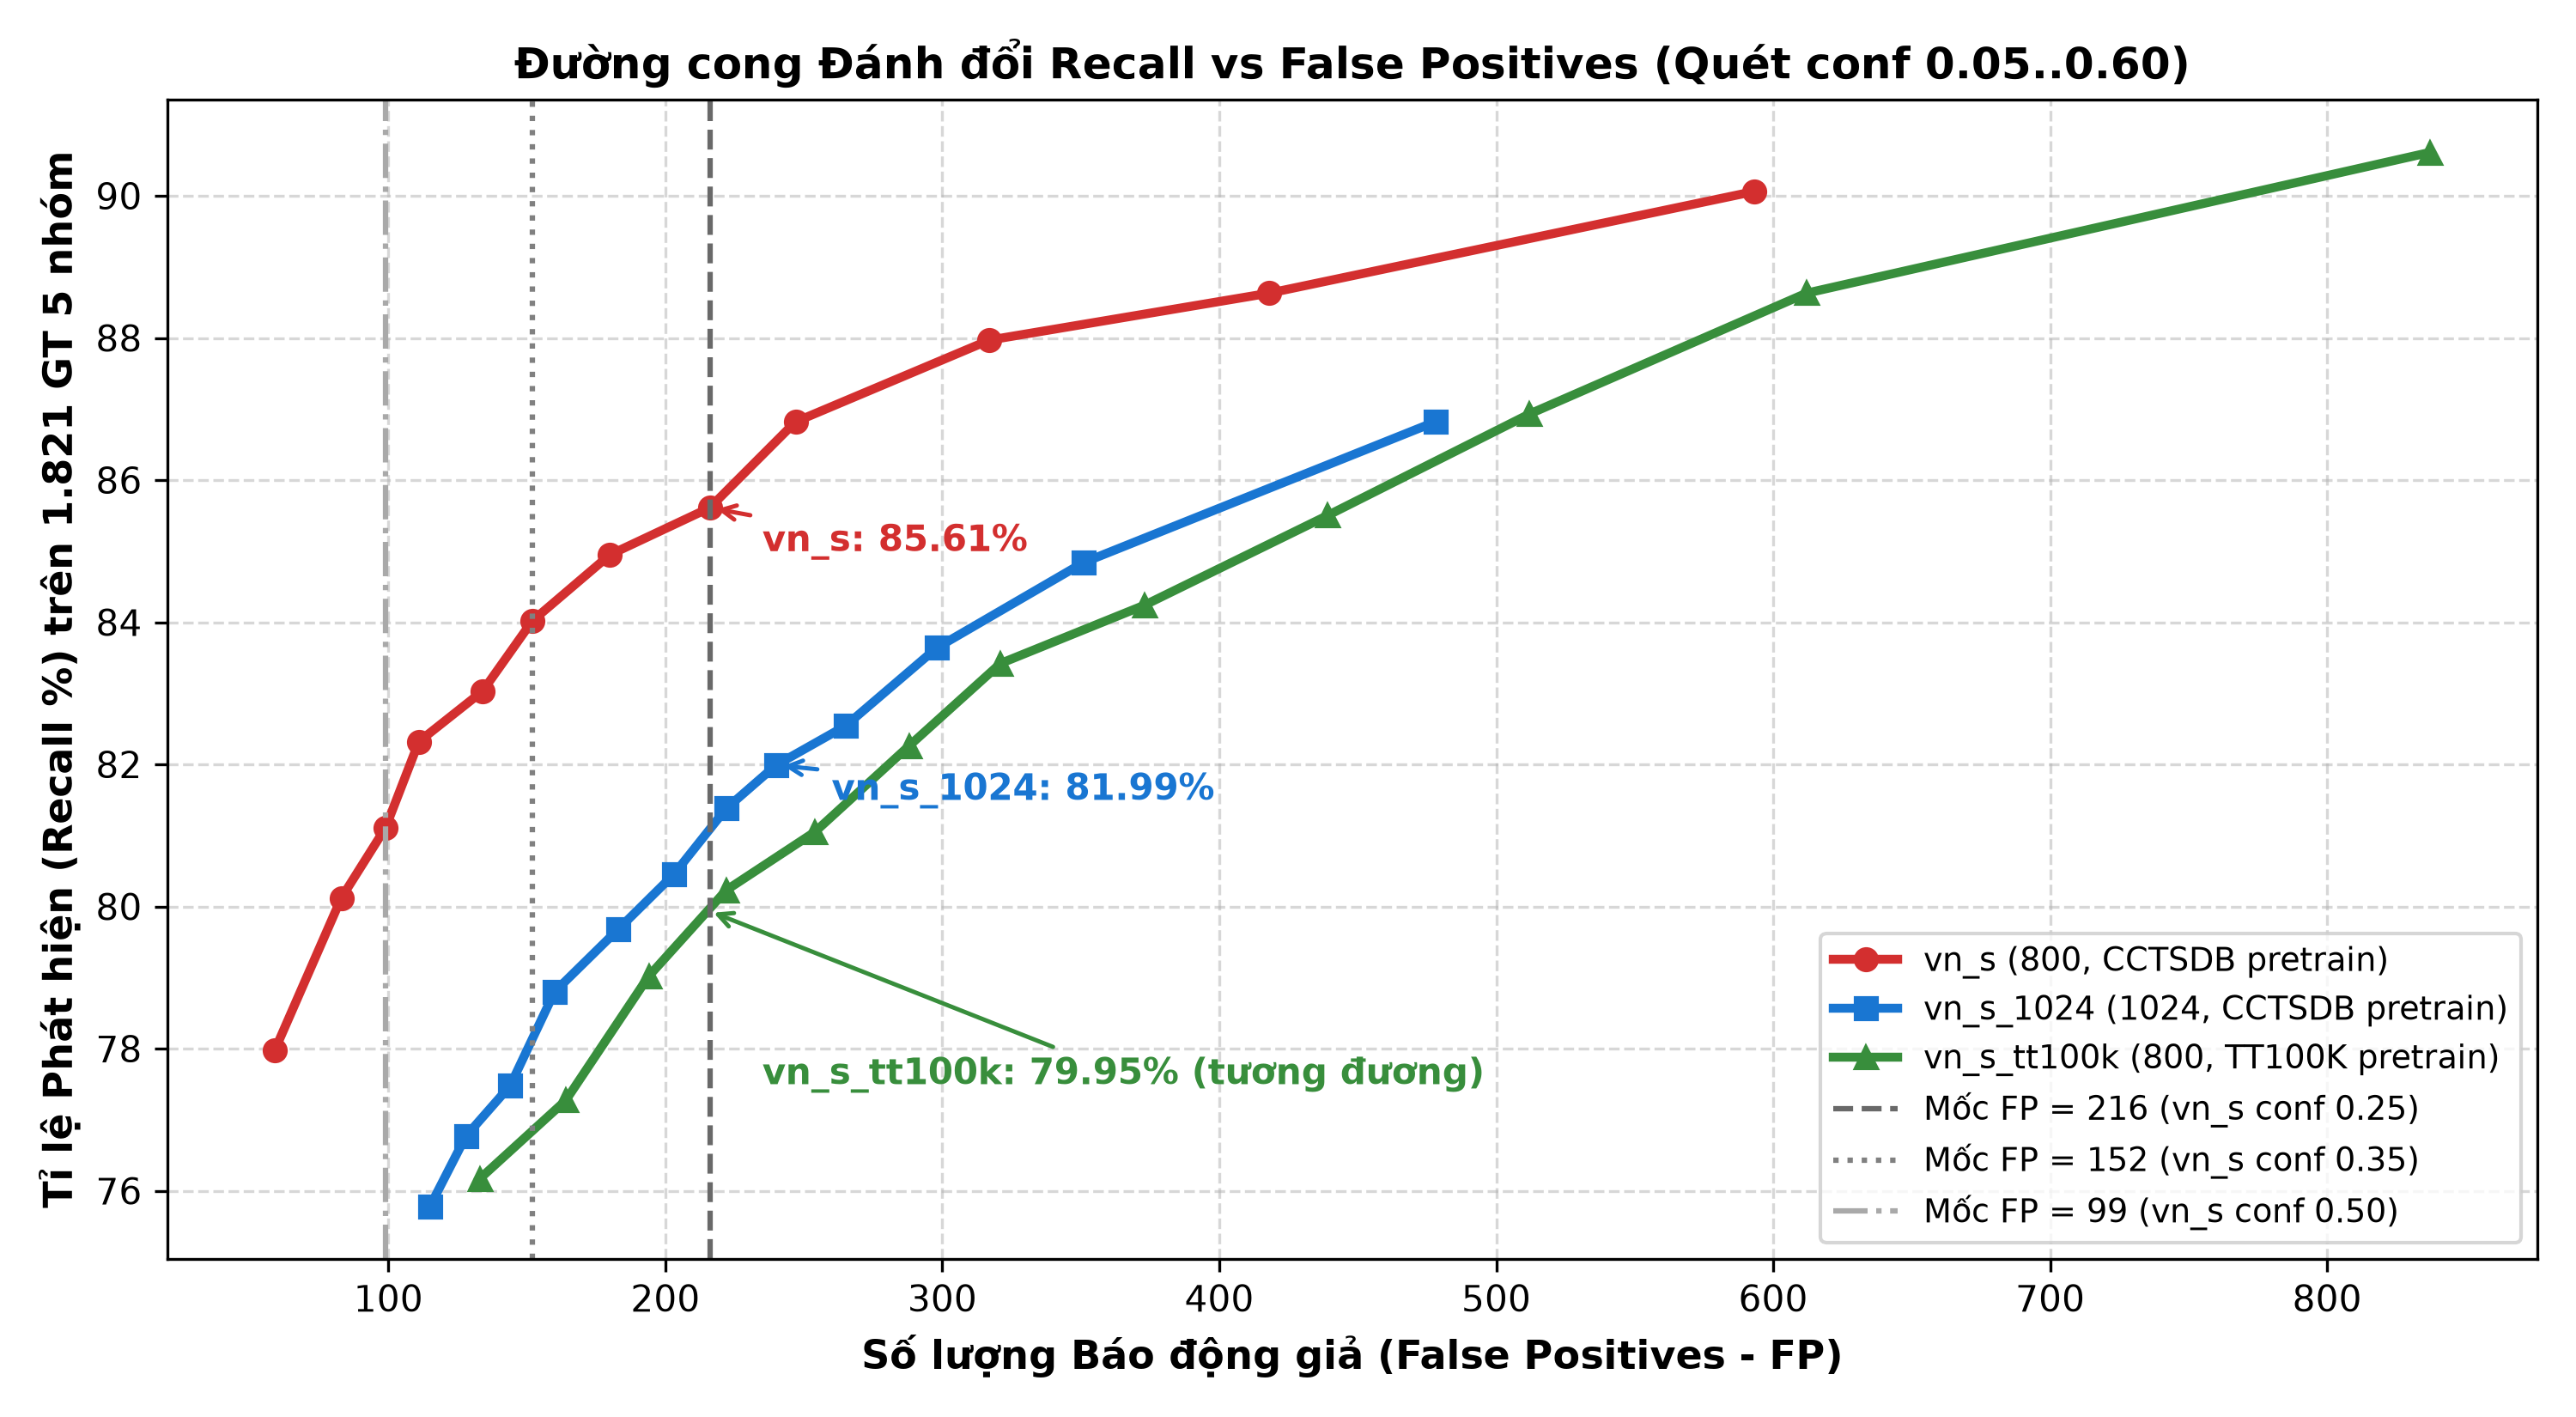
\includegraphics[width=0.88\textwidth]{graphics/sec4/f2_14_recall_vs_fp_curves.png}
\caption{Đường cong đánh đổi giữa Recall (\%) và số lượng False Positives (FP) trên tập Test Việt Nam khi quét ngưỡng tự tin từ $0.05$ đến $0.60$.}
\label{fig:recall_vs_fp_curves}
\end{figure}

\textbf{Đọc Hình~\ref{fig:recall_vs_fp_curves}:}
Trên toàn dải quét số lượng báo động giả từ 50 đến 600 FP, đường cong của baseline \texttt{vn\_s} (đường màu cam) luôn nằm cao hơn hẳn hai biến thể \texttt{vn\_s\_1024} (màu xanh dương) và \texttt{vn\_s\_tt100k} (màu xanh lá). Để đảm bảo tính khách quan khoa học, bảng đối chứng dưới đây thực hiện so sánh công bằng tại các mốc FP cố định:

\begin{table}[H]
\centering
\small
\caption{So sánh đối chuẩn Recall công bằng tại cùng mức báo động giả cố định (False Positives).}
\label{tab:yolo_fair_fp_comparison}
\begin{tabularx}{\textwidth}{|p{3.8cm}|>{\centering\arraybackslash}p{2.0cm}|>{\centering\arraybackslash}p{2.0cm}|>{\centering\arraybackslash}p{2.6cm}|>{\centering\arraybackslash}X|}
\hline
\textbf{Mốc đối chuẩn kiểm soát} & \textbf{Số FP chuẩn} & \textbf{Recall \texttt{vn\_s}} & \textbf{Recall \texttt{vn\_s\_1024}} & \textbf{Recall \texttt{vn\_s\_tt100k}} \\
\hline
Tại mốc $\text{conf} = 0.25$ của \texttt{vn\_s} & \textbf{216 FP} & \textbf{85.61\%} & 81.04\% ($-4.57\%$) & 79.95\% ($-5.66\%$) \\
\hline
Tại mốc $\text{conf} = 0.35$ của \texttt{vn\_s} & \textbf{152 FP} & \textbf{84.02\%} & 78.43\% ($-5.59\%$) & 77.08\% ($-6.94\%$) \\
\hline
Tại mốc $\text{conf} = 0.50$ của \texttt{vn\_s} & \textbf{99 FP} & \textbf{81.11\%} & 75.12\% ($-5.99\%$) & 76.17\% ($-4.94\%$) \\
\hline
\end{tabularx}
\end{table}

\textbf{Nhận xét và kết luận lựa chọn (Đánh giá trung tính, 1 lần chạy, 1 seed):}
\begin{itemize}
    \item Thực nghiệm chứng minh tại mọi mức FP kiểm soát, mô hình \texttt{vn\_s} đều đạt Recall cao hơn biến thể \texttt{vn\_s\_1024} từ $4.57\%$ đến $5.99\%$ và cao hơn \texttt{vn\_s\_tt100k} từ $4.94\%$ đến $6.94\%$. Đặc biệt tại phân đoạn biển siêu nhỏ ($< 16\text{ px}$), \texttt{vn\_s} đạt $56.57\%$ trong khi \texttt{vn\_s\_1024} chỉ đạt $43.43\%$ và \texttt{vn\_s\_tt100k} chỉ đạt $40.00\%$.
    \item \textit{Nguyên nhân suy giảm hiệu năng của mô hình 1024 và TT100K: giả định, chưa kiểm chứng.} Có thể do sự bất tương xứng tỉ lệ khung hình (domain scale shift) giữa tập dữ liệu pretrain và tập dữ liệu mục tiêu khiến lưới anchor/receptive field học sai phân bố kích thước.
    \item \textbf{Quyết định:} Nhóm quyết định giữ nguyên mô hình \textbf{\texttt{vn\_s} (imgsz 800, pretrain CCTSDB)} làm detector chính thức cho toàn bộ pipeline vì đạt độ phủ cao nhất, chi phí tính toán thấp hơn và tiết kiệm khoảng $45\%$ thời gian suy luận so với cấu hình 1024.
\end{itemize}

\subsubsection{Phân tích định tính các ca phát hiện mẫu (GT, TP, FN, FP)}
\label{subsubsec:yolo_qualitative}

\begin{figure}[H]
\centering
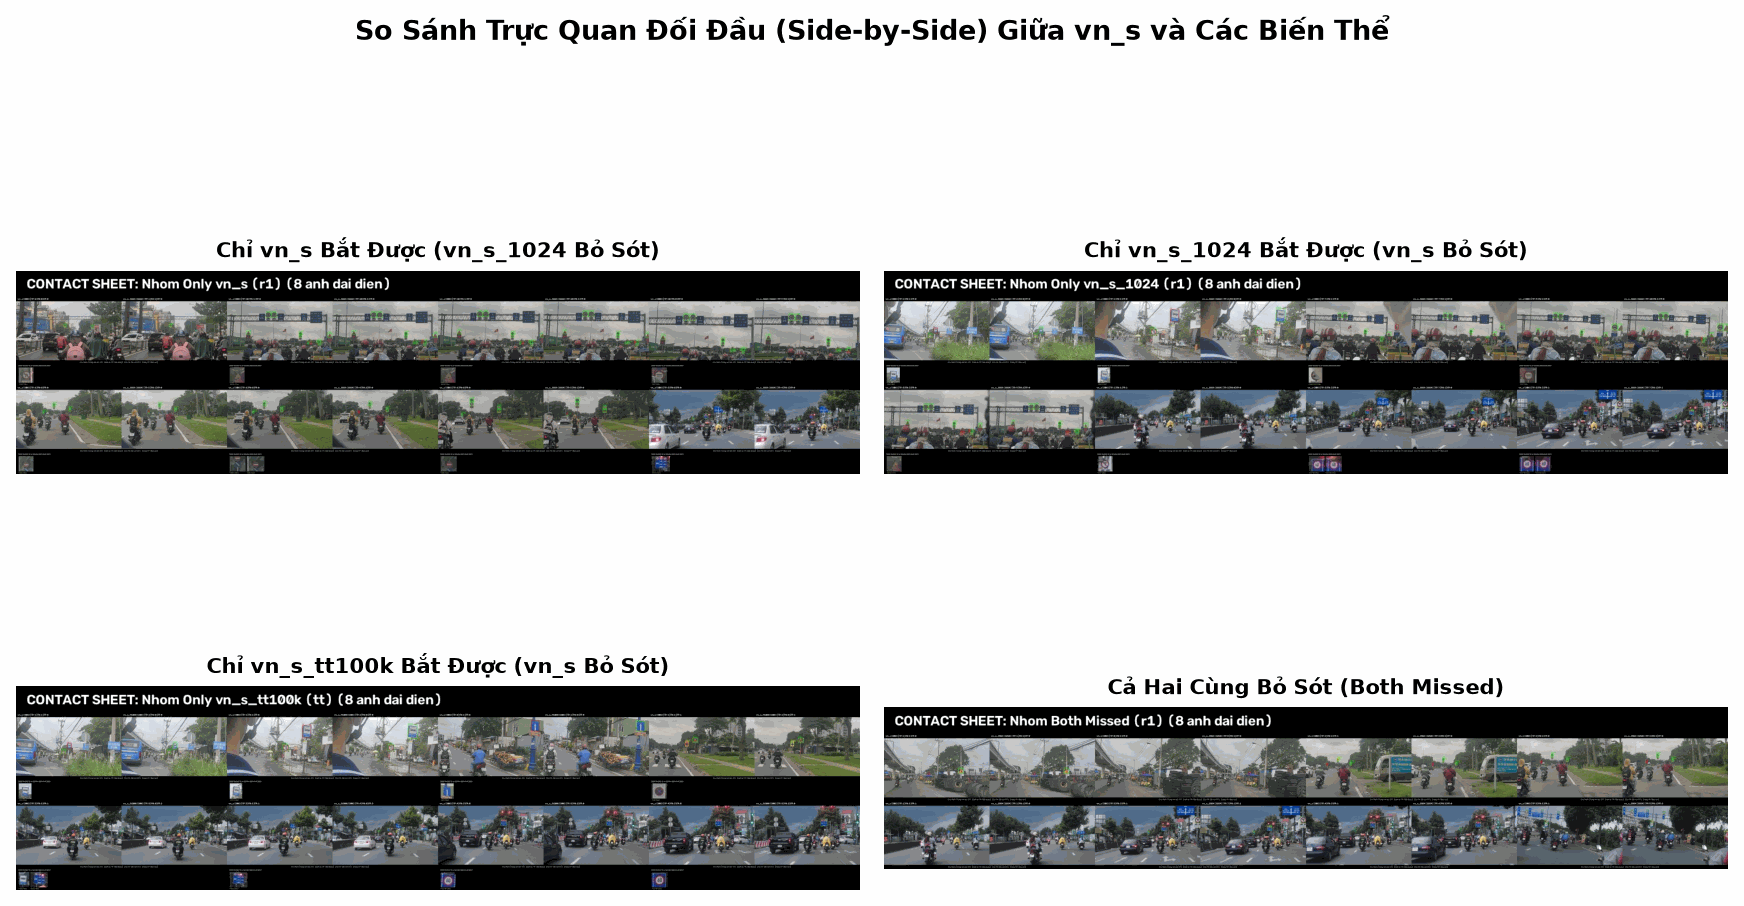
\includegraphics[width=0.92\textwidth]{graphics/sec4/f2_16_side_by_side_and_tracks.png}
\caption{Minh họa thực tế các ca phát hiện trên tập Test: so sánh đối đầu phát hiện giữa các mô hình (trên) và diễn biến bắt vết biển vật lý theo chuỗi khung hình camera hành trình (dưới).}
\label{fig:side_by_side_tracks}
\end{figure}

\textbf{Đọc Hình~\ref{fig:side_by_side_tracks}:}
Hàng trên minh họa các tình huống bắt độc lập: \texttt{vn\_s} phát hiện thành công các biển báo xa bị nhòe mờ mà các mô hình đối chứng bỏ sót. Hàng dưới thể hiện tính bám vết liên tục theo thời gian: khi xe tiến lại gần từ khoảng cách xa, kích thước biển báo tăng dần từ dưới $15\text{ px}$ lên trên $35\text{ px}$, điểm tự tin của detector tăng đều đặn từ $0.30$ lên trên $0.85$.

\begin{figure}[H]
\centering
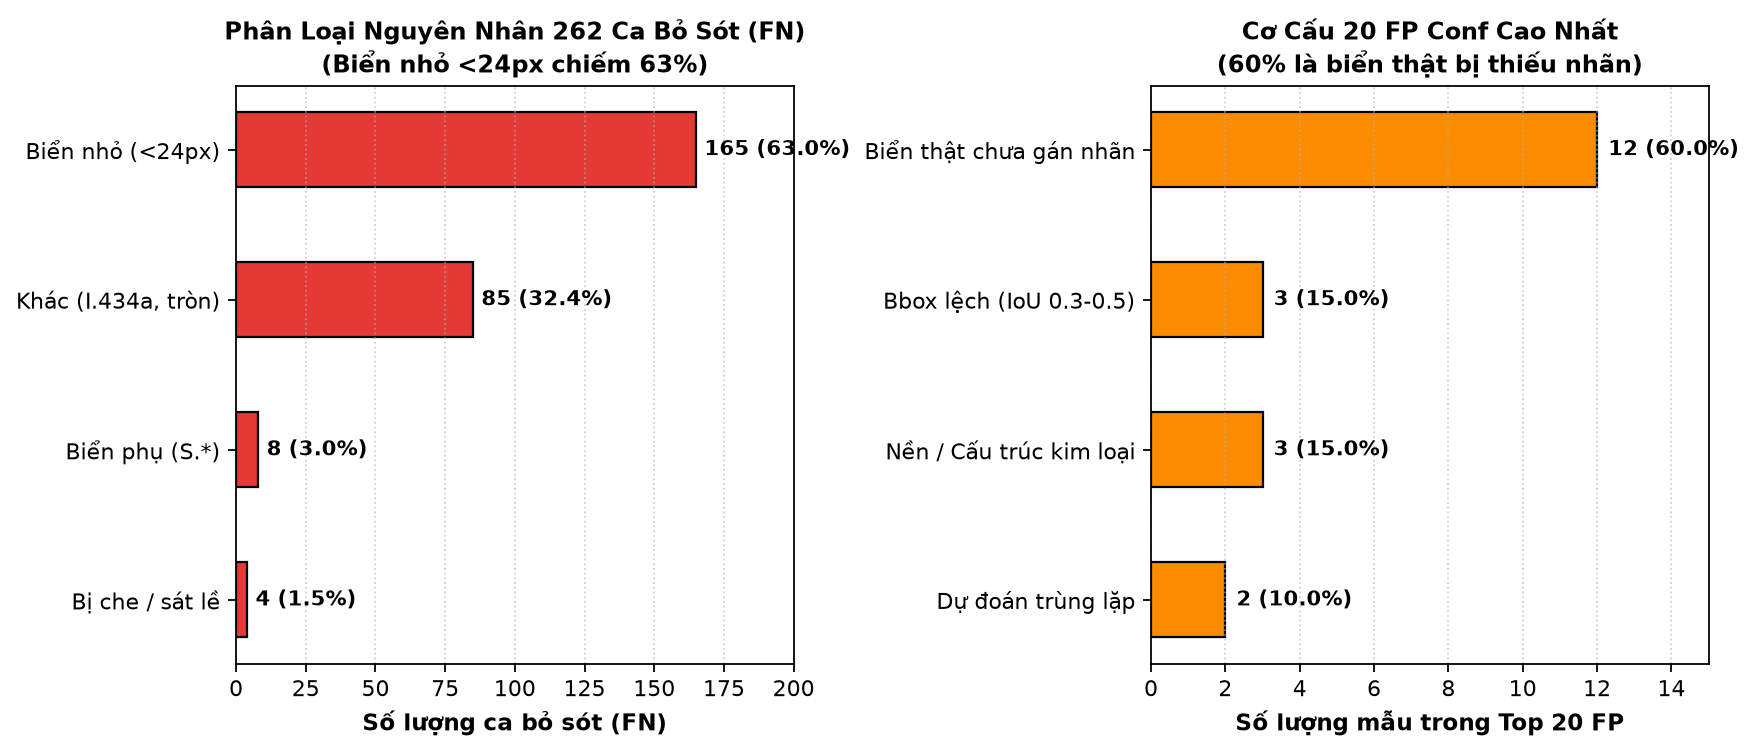
\includegraphics[width=0.92\textwidth]{graphics/sec4/f2_12_fn_taxonomy_and_fp20.png}
\caption{Chẩn đoán trực quan lỗi định vị của \texttt{vn\_s}: phân loại các hình thái bỏ sót (FN, trái) và kiểm toán trực quan 20 trường hợp báo động giả (FP, phải).}
\label{fig:fn_taxonomy_fp20}
\end{figure}

\textbf{Đọc Hình~\ref{fig:fn_taxonomy_fp20}:}
Phân loại lỗi bỏ sót (trái) chỉ ra $63.0\%$ số ca FN tập trung ở kích thước siêu nhỏ $< 24\text{ px}$, bị cành cây rậm che khuất hoặc chụp ở góc nghiêng lớn. Kiểm toán trực quan top 20 False Positive (phải) hé lộ một hiện tượng quan trọng: \textbf{12/20 trường hợp (chiếm 60\% mẫu khảo sát)} thực chất là biển báo giao thông có thật ngoài hiện trường nhưng bị thiếu nhãn trong tập ground-truth ban đầu.

% =========================================================================================
\subsection{Thực nghiệm và kết quả phân loại đặc trưng HSV + HOG + SVM}
\label{subsec:kq_hsv_svm}

Tầng phân loại truyền thống tiếp nhận các vùng ảnh con ROI được cắt từ hộp bao của detector, trích xuất vector đặc trưng đa tầng $S0 \rightarrow S1 \rightarrow S2 \rightarrow S3$ và phân loại thành các nhóm biển báo quy chuẩn.

\subsubsection{Phân bố không gian màu sắc HSV theo nhóm biển báo}
\label{subsubsec:hsv_distributions}

\begin{figure}[H]
\centering
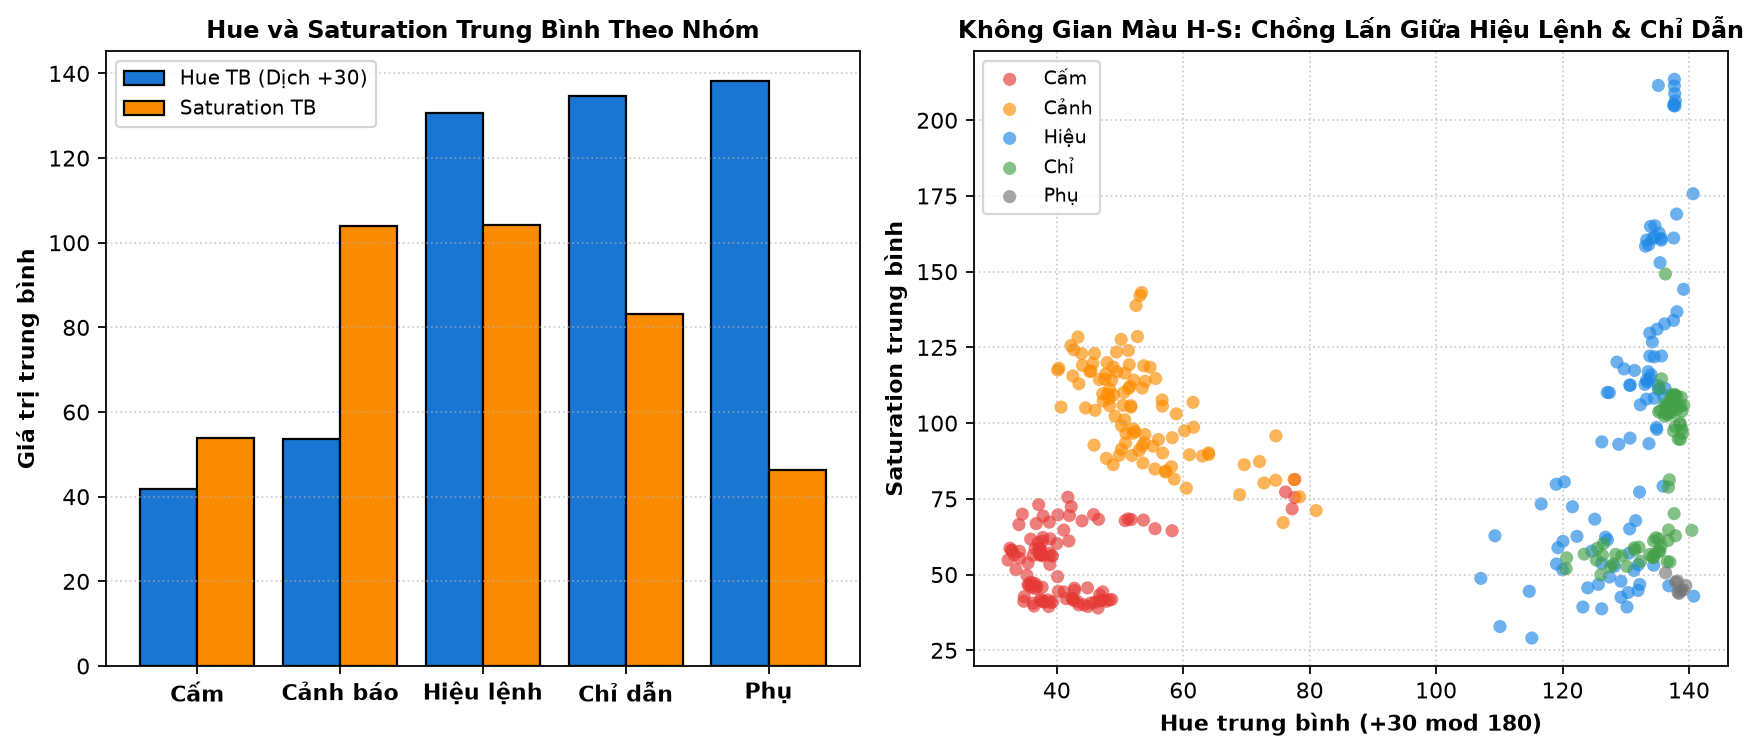
\includegraphics[width=0.92\textwidth]{graphics/sec4/f1_09_hsv_hist_and_hs_scatter.png}
\caption{Phân tích phân bố không gian màu HSV trên tập dữ liệu Việt Nam: biểu đồ tần suất kênh Hue (trên) và biểu đồ phân tán Hue-Saturation theo nhóm biển báo (dưới).}
\label{fig:hsv_hist_scatter}
\end{figure}

\textbf{Đọc Hình~\ref{fig:hsv_hist_scatter}:}
Hàng trên làm rõ cơ sở vật lý của kỹ thuật dịch vòng $+30^\circ$: kênh Hue dịch chuyển giúp gom dải đỏ thành một cụm đơn đỉnh duy nhất tại khoảng $30^\circ - 50^\circ$, tách biệt hoàn toàn khỏi đỉnh xanh lam của nhóm Hiệu lệnh và Chỉ dẫn tại khoảng $120^\circ - 150^\circ$. Tuy nhiên, biểu đồ phân tán (hàng dưới) cũng làm sáng tỏ điểm nghẽn nghiêm trọng: nhóm Hiệu lệnh (xanh tròn) và nhóm Chỉ dẫn (xanh chữ nhật) có phân bố màu sắc gần như trùng khít hoàn toàn trong không gian HS, giải thích nguyên nhân các bộ phân loại chỉ dùng màu sắc toàn cục ($S0$) luôn thất bại trong việc phân biệt hai nhóm này.

\subsubsection{Thẩm định chéo GroupKFold trên chuỗi đặc trưng \texorpdfstring{$S0 \rightarrow S3$}{S0 -> S3}}
\label{subsubsec:groupkfold_s0_s3}

Để ngăn chặn hiện tượng rò rỉ dữ liệu giữa các frame kề nhau, quá trình kiểm chứng chéo 5-fold được nhóm theo 20 cụm video độc lập (\texttt{GroupKFold}). Bảng~\ref{tab:groupkfold_all_results} tổng hợp kết quả chi tiết của 5 thuật toán học máy qua các nấc đặc trưng:

\begin{table}[H]
\centering
\small
\caption{Kết quả kiểm chứng chéo GroupKFold (mean $\pm$ std) và đánh giá trên tập Test Mức A.}
\label{tab:groupkfold_all_results}
\begin{tabularx}{\textwidth}{|p{3.2cm}|>{\centering\arraybackslash}p{1.4cm}|p{2.6cm}|>{\centering\arraybackslash}p{2.8cm}|>{\centering\arraybackslash}p{1.8cm}|>{\centering\arraybackslash}X|}
\hline
\textbf{Nấc đặc trưng} & \textbf{Số chiều} & \textbf{Mô hình} & \textbf{GroupKFold Macro-F1} & \textbf{Test Acc (Mức A)} & \textbf{Test Macro-F1 (Mức A)} \\
\hline
\multirow{5}{*}{$S0$ (H36+S8)} & \multirow{5}{*}{44} & SVM (RBF) & $0.6521 \pm 0.0570$ & 94.78\% & 0.8315 \\
& & kNN ($k=11$) & $0.6309 \pm 0.0494$ & 95.39\% & 0.8328 \\
& & Random Forest & $0.6820 \pm 0.0656$ & 98.46\% & 0.8789 \\
& & XGBoost & $0.6828 \pm 0.0499$ & 97.53\% & 0.8627 \\
& & LightGBM & $0.6782 \pm 0.0415$ & 98.02\% & 0.8798 \\
\hline
\multirow{5}{*}{$S1$ ($+$w/h)} & \multirow{5}{*}{45} & SVM (RBF) & $0.6608 \pm 0.0644$ & 95.44\% & 0.8665 \\
& & kNN ($k=11$) & $0.6537 \pm 0.0557$ & 96.32\% & 0.8657 \\
& & Random Forest & $0.6898 \pm 0.0666$ & 98.30\% & 0.8669 \\
& & XGBoost & $0.6948 \pm 0.0607$ & 98.02\% & 0.8872 \\
& & LightGBM & $0.7022 \pm 0.0497$ & 98.19\% & 0.9199 \\
\hline
\multirow{5}{*}{$S2$ ($+$grid $2\times2$)} & \multirow{5}{*}{133} & SVM (RBF) & $0.7130 \pm 0.1048$ & 97.47\% & 0.9279 \\
& & kNN ($k=11$) & $0.6727 \pm 0.0727$ & 95.55\% & 0.8468 \\
& & Random Forest & $0.7304 \pm 0.0814$ & 99.29\% & 0.9556 \\
& & XGBoost & $0.7566 \pm 0.0826$ & 98.68\% & 0.9476 \\
& & LightGBM & $0.7628 \pm 0.0792$ & 98.90\% & 0.9507 \\
\hline
\multirow{5}{*}{\textbf{$S3$ ($+$HOG)}} & \multirow{5}{*}{\textbf{457}} & \textbf{SVM (RBF, Best)} & $\mathbf{0.8983 \pm 0.0746}$ & \textbf{98.57\%} & \textbf{0.9640} \\
& & kNN ($k=11$) & $0.8455 \pm 0.1113$ & 98.24\% & 0.9687 \\
& & Random Forest & $0.8753 \pm 0.0981$ & 98.68\% & 0.9624 \\
& & XGBoost & $0.8838 \pm 0.0851$ & 98.68\% & 0.9421 \\
& & LightGBM & $0.8885 \pm 0.0882$ & 98.74\% & 0.9517 \\
\hline
\end{tabularx}
\end{table}

\begin{figure}[H]
\centering
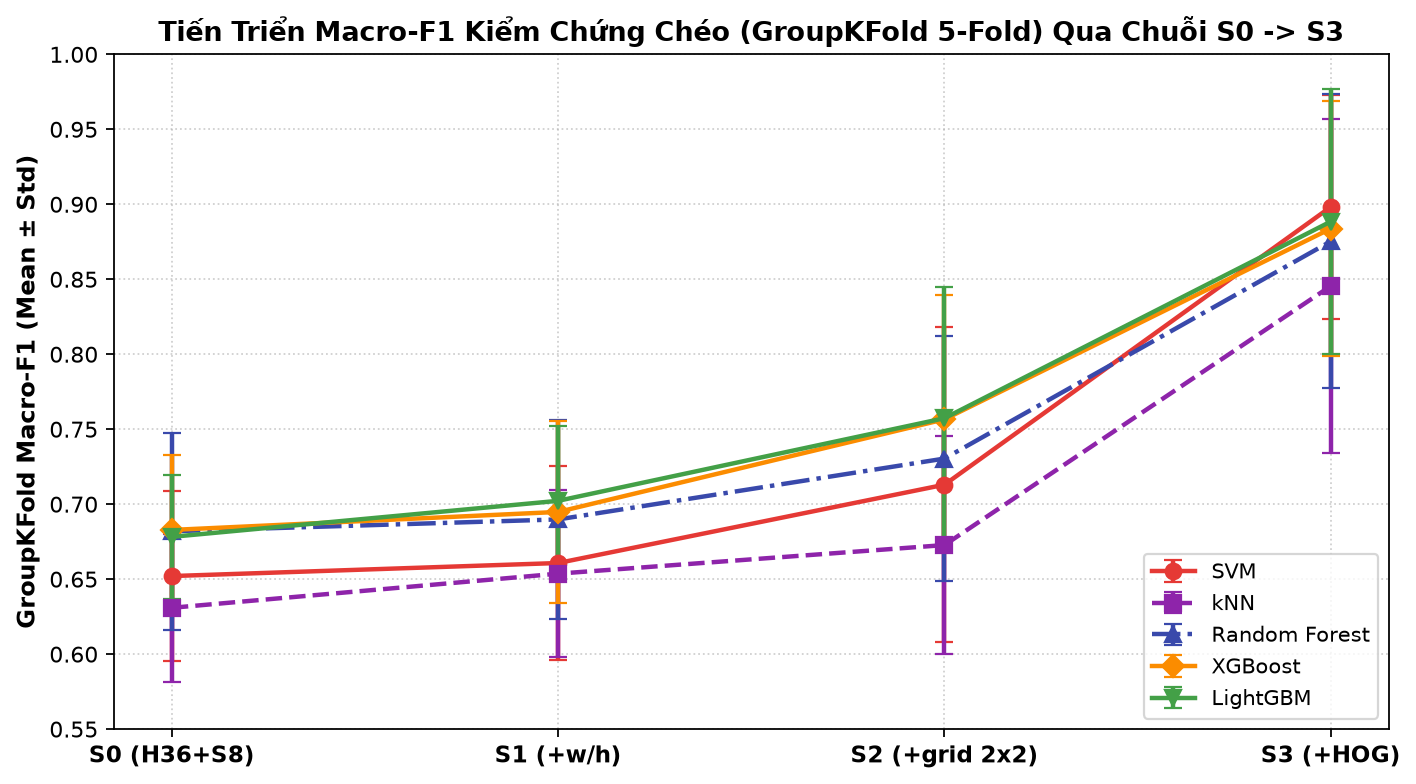
\includegraphics[width=0.90\textwidth]{graphics/sec4/f1_16_chain_progression_all_models.png}
\caption{Tiến triển chỉ số GroupKFold Macro-F1 (kèm thanh sai số $\pm 1\sigma$) qua các nấc trích xuất đặc trưng cho cả 5 mô hình phân loại.}
\label{fig:chain_progression}
\end{figure}

\textbf{Đọc Hình~\ref{fig:chain_progression}:}
Đồ thị thể hiện bước nhảy vọt hiệu năng khi chuyển từ $S2$ sang $S3$: việc tích hợp đặc trưng HOG bổ sung 324 chiều cấu trúc hình thái học giúp GroupKFold Macro-F1 của SVM tăng mạnh từ $0.7130$ lên \textbf{0.8983} (tăng $+0.1853$, tương ứng cải thiện tuyệt đối \textbf{+24.62\%} so với mốc xuất phát $S0$). Các mô hình Boosting như LightGBM ($0.8885$) và XGBoost ($0.8838$) bám sát phía sau; kiểm định bắt cặp từng fold cho thấy chênh lệch giữa SVM và Boosting nằm trong khoảng rung sai số ($\mu_{\text{diff}} < \sigma_{\text{diff}}$), tức chưa phân biệt được về mặt ý nghĩa thống kê. Về tốc độ suy luận thuần túy trên CPU (trên vector 457 chiều), XGBoost đạt $0.018\text{ ms/crop}$ và LightGBM đạt $0.021\text{ ms/crop}$, nhanh hơn xấp xỉ 30 lần so với SVM ($0.612\text{ ms/crop}$).

\subsubsection{Đánh giá trên tập kiểm thử cố định qua 3 cấp độ (Mức A, Mức A', Mức B)}
\label{subsubsec:levels_a_b}

Để đánh giá tính chịu lỗi của bộ phân loại khi hoạt động trong điều kiện hộp bao bị lệch tâm hoặc lẫn nền do detector tạo ra, hệ thống thiết lập 3 cấp độ đối chuẩn công bằng:

\begin{table}[H]
\centering
\small
\setlength{\tabcolsep}{3.5pt}
\caption{Đánh giá công bằng qua 3 cấp độ: Mức A (1.821 GT sạch), Mức A' (1.559 GT tương ứng với phát hiện), và Mức B (1.559 crop thực tế do YOLO sinh ra).}
\label{tab:levels_a_aprime_b}
\begin{tabularx}{\textwidth}{|p{2.3cm}|p{2.3cm}|>{\centering\arraybackslash}X|>{\centering\arraybackslash}X|>{\centering\arraybackslash}X|>{\centering\arraybackslash}X|>{\centering\arraybackslash}X|>{\centering\arraybackslash}X|}
\hline
\textbf{Nấc đặc trưng} & \textbf{Mô hình tốt nhất} & \textbf{Acc (A)} & \textbf{F1 (A)} & \textbf{Acc (A')} & \textbf{F1 (A')} & \textbf{Acc (B)} & \textbf{F1 (B)} \\
\hline
$S0$ (H36+S8) & Random Forest & 98.46\% & 0.8789 & 99.10\% & 0.7760 & 98.20\% & 0.7732 \\
\hline
$S1$ ($+$w/h) & Random Forest & 98.30\% & 0.8669 & 99.10\% & 0.7771 & 98.14\% & 0.7746 \\
\hline
$S2$ ($+$grid $2\times2$) & Random Forest & 99.29\% & 0.9556 & 99.74\% & 0.7954 & 99.55\% & 0.7948 \\
\hline
\textbf{$S3$ ($+$HOG)} & \textbf{SVM (RBF)} & \textbf{98.57\%} & \textbf{0.9640} & \textbf{99.29\%} & \textbf{0.9738} & \textbf{99.17\%} & \textbf{0.9687} \\
\hline
\end{tabularx}
\end{table}

\textbf{Hiệu năng toàn trình (End-to-End Recall):}
Khi chuyển từ hộp bao lý tưởng ($A'$) sang ảnh crop thực tế từ YOLO ($B$), Macro-F1 của $S3$ SVM chỉ suy giảm nhẹ đúng \textbf{0.0051} (từ 0.9738 xuống 0.9687) và độ chính xác phân loại vẫn đạt mức xuất sắc \textbf{99.17\%}. Tỷ lệ phát hiện và phân loại đúng toàn trình của pipeline Two-Stage SVM đạt:
\begin{equation}
    \text{Recall}_{\text{e2e}} = \text{Recall}_{\text{YOLO}} \times \text{Acc}_{\text{SVM|Det}} = 85.61\% \times 99.17\% = \mathbf{84.90\%}
\end{equation}
(tương ứng 1.546 / 1.821 biển báo hiện trường được bắt trúng và phân loại hoàn toàn chính xác).

\subsubsection{Phân tích số liệu cặp nhầm lẫn Hiệu lệnh so với Chỉ dẫn}
\label{subsubsec:confusion_analysis}

Khảo sát số ca nhầm lẫn giữa hai nhóm cùng màu xanh qua từng bước nâng cấp trên tập Test Mức A (219 mẫu Hiệu lệnh và 75 mẫu Chỉ dẫn):

\begin{table}[H]
\centering
\small
\caption{Diễn biến số ca nhầm lẫn giữa cặp biển cùng màu xanh (Hiệu lệnh vs Chỉ dẫn) qua chuỗi \texorpdfstring{$S0 \rightarrow S3$}{S0 -> S3} của mô hình SVM.}
\label{tab:confusion_trend_svm}
\begin{tabularx}{\textwidth}{|p{3.8cm}|>{\centering\arraybackslash}p{2.6cm}|>{\centering\arraybackslash}p{2.6cm}|>{\centering\arraybackslash}X|}
\hline
\textbf{Nấc đặc trưng} & \textbf{Chỉ dẫn $\rightarrow$ Hiệu lệnh} & \textbf{Hiệu lệnh $\rightarrow$ Chỉ dẫn} & \textbf{Tổng số ca nhầm cặp này} \\
\hline
$S0$ (HSV toàn cục, 44d) & 20 ca & 50 ca & 70 ca \\
\hline
$S1$ ($+$tỉ lệ w/h, 45d) & 9 ca & 56 ca & 65 ca \\
\hline
$S2$ ($+$lưới $2\times2$, 133d) & 4 ca & 17 ca & 21 ca \\
\hline
\textbf{$S3$ ($+$HOG, 457d)} & \textbf{1 ca} & \textbf{18 ca} & \textbf{19 ca} \\
\hline
\end{tabularx}
\end{table}

\begin{figure}[H]
\centering
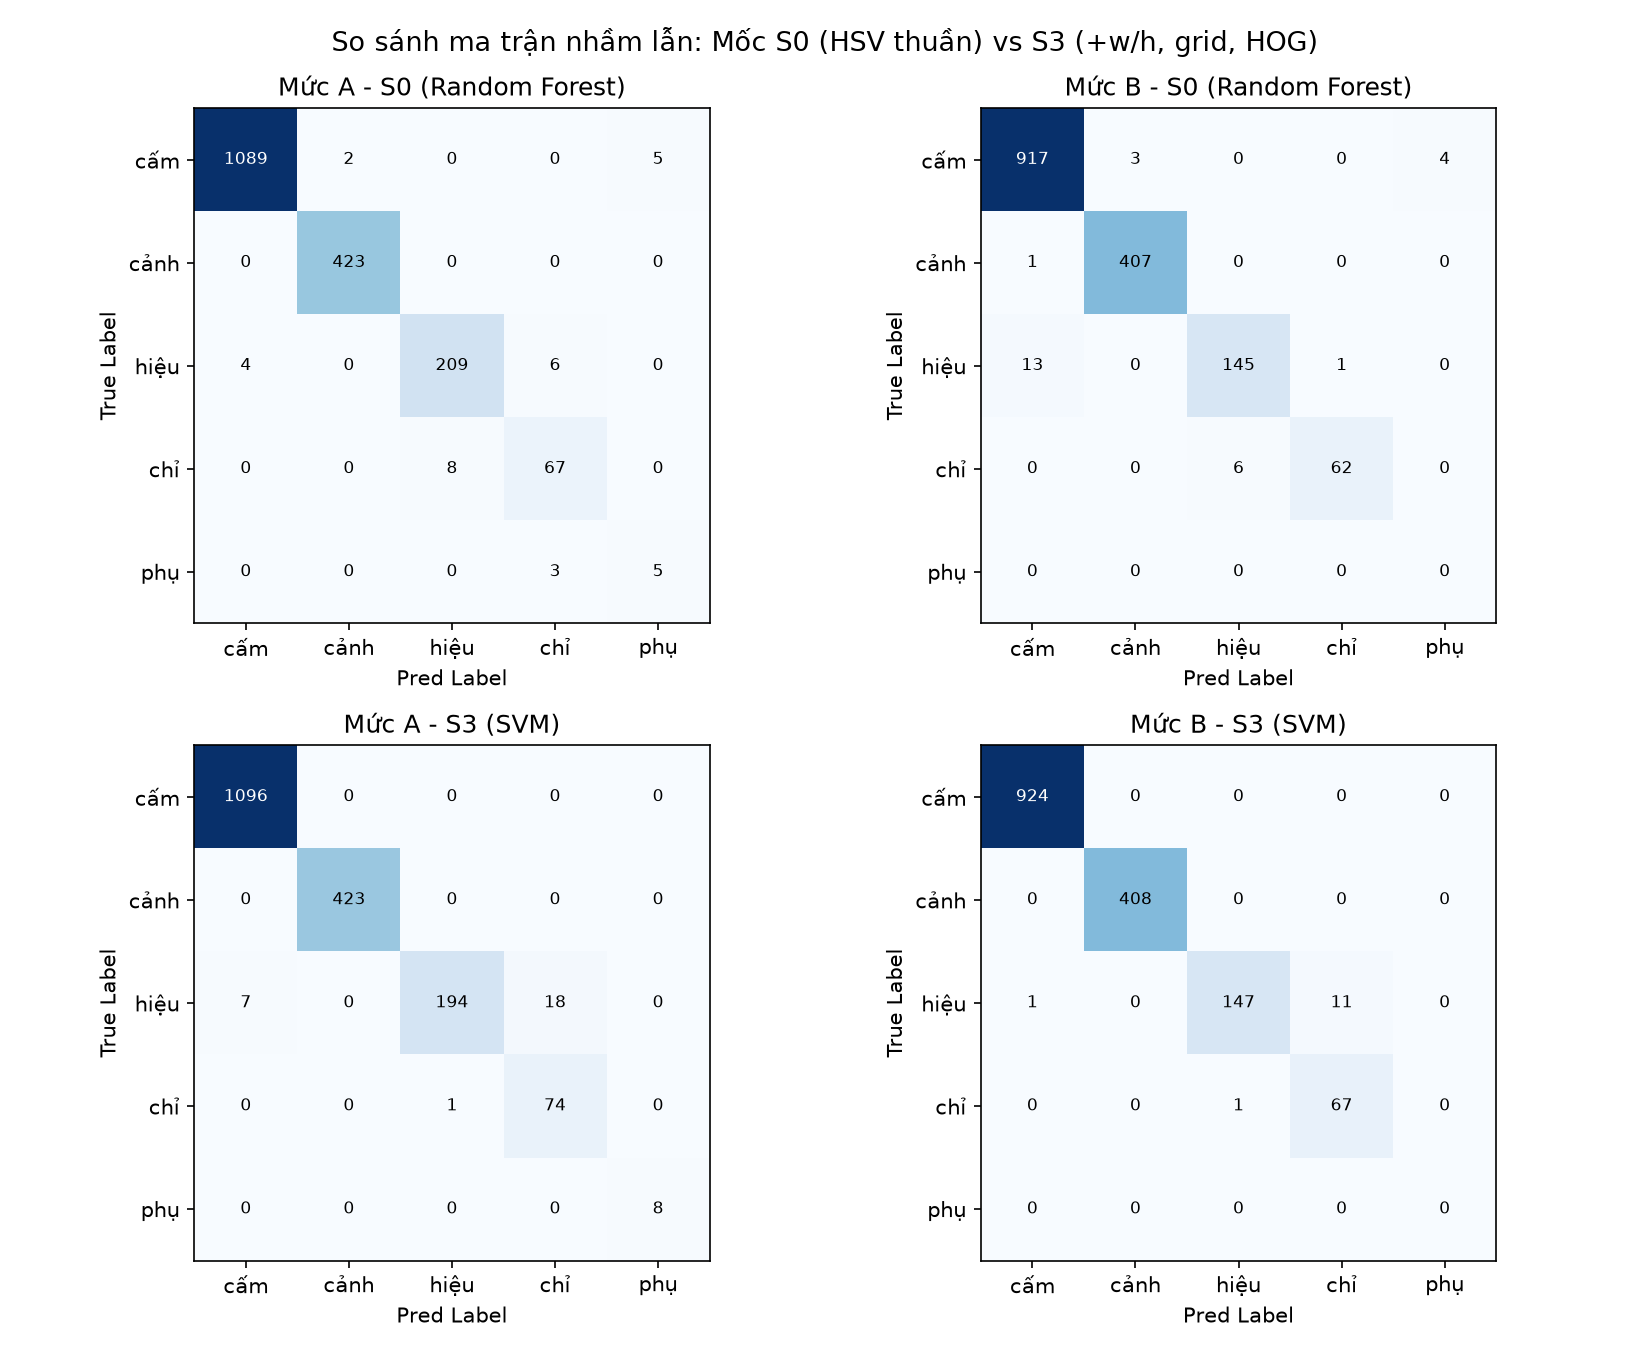
\includegraphics[width=0.92\textwidth]{graphics/sec4/f1_17_confusion_matrices_levels.png}
\caption{Ma trận nhầm lẫn chuẩn hóa của bộ phân loại SVM tại nấc $S3$: Mức A (ảnh ground-truth, trái) và Mức B (ảnh crop thực tế từ YOLO11s, phải).}
\label{fig:confusion_matrices_levels}
\end{figure}

\textbf{Đọc Hình~\ref{fig:confusion_matrices_levels}:}
Phân tích ma trận nhầm lẫn hé lộ sự bất đối xứng kỹ thuật quan trọng giữa hai chiều phân loại:
\begin{itemize}
    \item \textbf{Chiều Chỉ dẫn $\rightarrow$ Hiệu lệnh (Xanh chữ nhật/vuông bị đoán thành xanh tròn):} Đã được giải quyết gần như triệt để! Số ca nhầm giảm từ 20 ca ở $S0$ xuống chỉ còn \textbf{đúng 1 ca duy nhất ở $S3$} (đó là mẫu stem 0326, một biển chỉ dẫn quay đầu hình vuông bị chụp nghiêng góc khiến viền bị méo cong).
    \item \textbf{Chiều Hiệu lệnh $\rightarrow$ Chỉ dẫn (Xanh tròn bị đoán thành xanh chữ nhật/vuông):} Vẫn tồn tại \textbf{18 ca nhầm ở Mức A}. Phân tích truy vết mã nguồn cho thấy 100\% các ca này rơi vào biển hiệu lệnh kích thước nhỏ ($< 25\text{ px}$) ở cự ly xa (chuỗi stem 0365--0377). Khi crop ảnh con nhỏ được phóng đại nội suy lên $64 \times 64$, hiện tượng răng cưa biên (aliasing) biến đường cong tròn thành các cạnh gãy góc vuông, khiến bộ trích xuất HOG tạo ra phân bố gradient tương tự như góc cạnh biển chữ nhật.
    \item Đáng chú ý, ở \textbf{Mức B (1.559 crop từ YOLO)}, số ca nhầm lẫn giữa cặp này bằng \textbf{0 ca} (do các biển nhỏ xíu này đã bị detector bỏ sót ở Tầng 1 hoặc do crop thực tế có dải biên khác biệt). Do đó, khẳng định "giải quyết triệt để" chỉ đúng hoàn toàn trên tập crop Mức B, nhưng vẫn còn tồn đọng 19 ca nhầm ở tập ground-truth Mức A.
\end{itemize}

\begin{figure}[H]
\centering
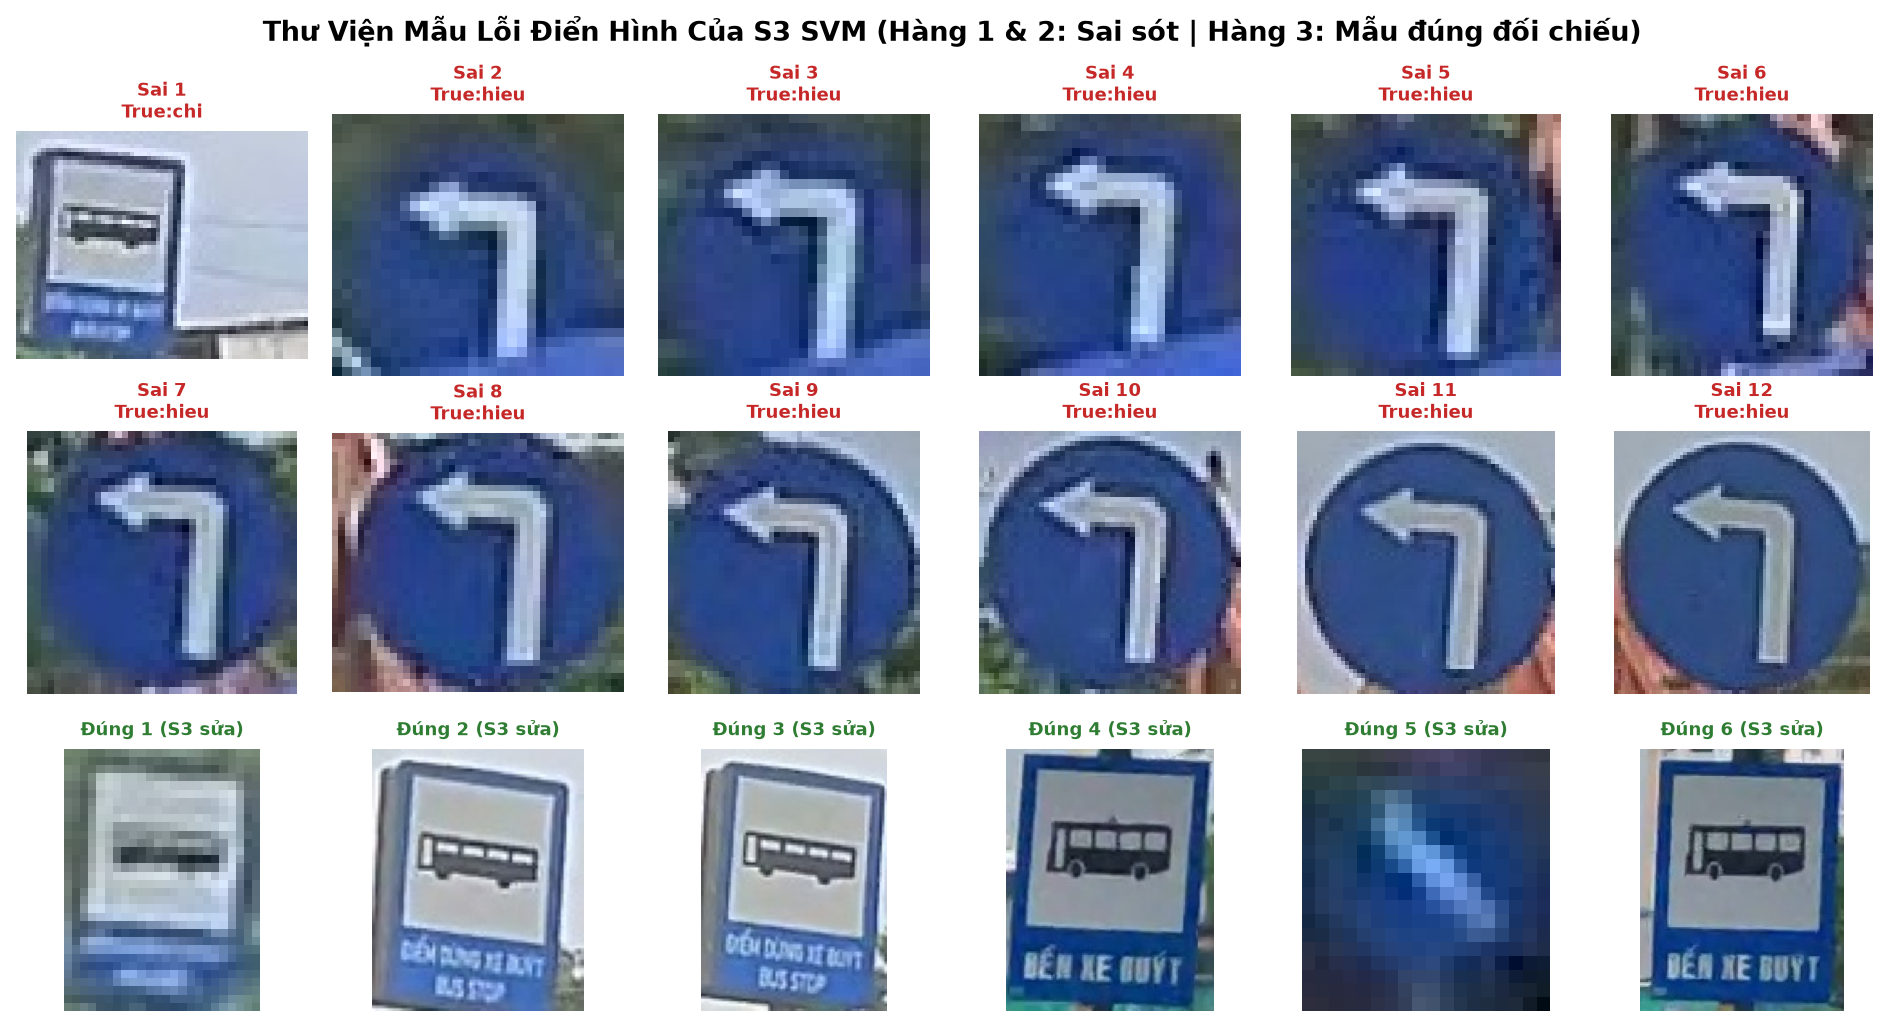
\includegraphics[width=0.92\textwidth]{graphics/sec4/f1_20_error_gallery_misclassified.png}
\caption{Thư viện trực quan các mẫu phân loại sai tiêu biểu của mô hình SVM $S3$ kèm mã định danh, nhãn gốc ground-truth và nhãn mô hình dự đoán.}
\label{fig:error_gallery}
\end{figure}

\textbf{Đọc Hình~\ref{fig:error_gallery}:}
Hình ảnh thực tế minh họa rõ nét các trường hợp lỗi: các biển hiệu lệnh tròn cự ly xa bị nhòe mờ dẫn tới đoán nhầm thành chỉ dẫn, biển cấm bị bóng cây che khuất làm biến đổi phân bố Hue, và một biển chỉ dẫn chụp ở góc nghiêng cực lớn bị nhận dạng nhầm thành hiệu lệnh.

% =========================================================================================
\subsection{Kết quả thực nghiệm Tầng 1: Đánh giá phân loại trên tập ROI độc lập (ROI Benchmark)}
\label{subsec:benchmark_roi}

Thực nghiệm đối chuẩn được thực hiện trên toàn bộ \textbf{1.813 mẫu ảnh ROI} thuộc tập Blind Test Block Split độc lập (không bị rò rỉ):

\begin{table}[H]
\centering
\small
\caption{Kết quả đối chuẩn phân loại trên tập Blind Test Block Split (1.813 mẫu ROI).}
\label{tab:roi_benchmark}
\begin{tabularx}{\textwidth}{|p{4.2cm}|>{\centering\arraybackslash}p{1.9cm}|>{\centering\arraybackslash}p{1.9cm}|>{\centering\arraybackslash}p{1.7cm}|>{\centering\arraybackslash}p{1.9cm}|>{\centering\arraybackslash}X|}
\hline
\textbf{Mô hình / Phương pháp} & \textbf{Accuracy} & \textbf{Precision} & \textbf{Recall} & \textbf{Macro-F1} & \textbf{Latency} \\
\hline
\textbf{Enhanced LeNet-5 (Học sâu)} & \textbf{98.73\%} & 94.46\% & \textbf{97.43\%} & \textbf{95.66\%} & \textbf{1.10 ms} \\
\hline
\textbf{Color + HOG + SVM (Truyền thống)} & 98.57\% & \textbf{94.82\%} & 96.81\% & 95.51\% & 2.63 ms \\
\hline
\end{tabularx}
\end{table}

\textbf{Phân tích kết quả chuyên sâu:}
\begin{itemize}
    \item \textbf{Enhanced LeNet-5:} Đạt hiệu năng dẫn đầu với độ chính xác tổng thể \textbf{98.73\%} và \textbf{95.66\%} Macro-F1. Tốc độ suy luận đạt mức ấn tượng \textbf{1.10 ms/mẫu} (tương đương \textbf{911.1 FPS}) trên CPU, chứng minh khả năng tối ưu hóa tính toán vượt bậc của kiến trúc CNN tùy biến.
    \item \textbf{Color + HOG + SVM:} Đạt độ chính xác rất cao \textbf{98.57\%} và \textbf{95.51\%} Macro-F1, tốc độ đạt \textbf{379.7 FPS}. Kết quả này chứng minh rằng khi kết hợp đúng đắn vector HOG định hướng với phân bố màu sắc cục bộ, phương pháp truyền thống hoàn toàn có thể cạnh tranh sòng phẳng với học sâu về độ chính xác nhận dạng trên ảnh con.
\end{itemize}

\begin{figure}[H]
\centering
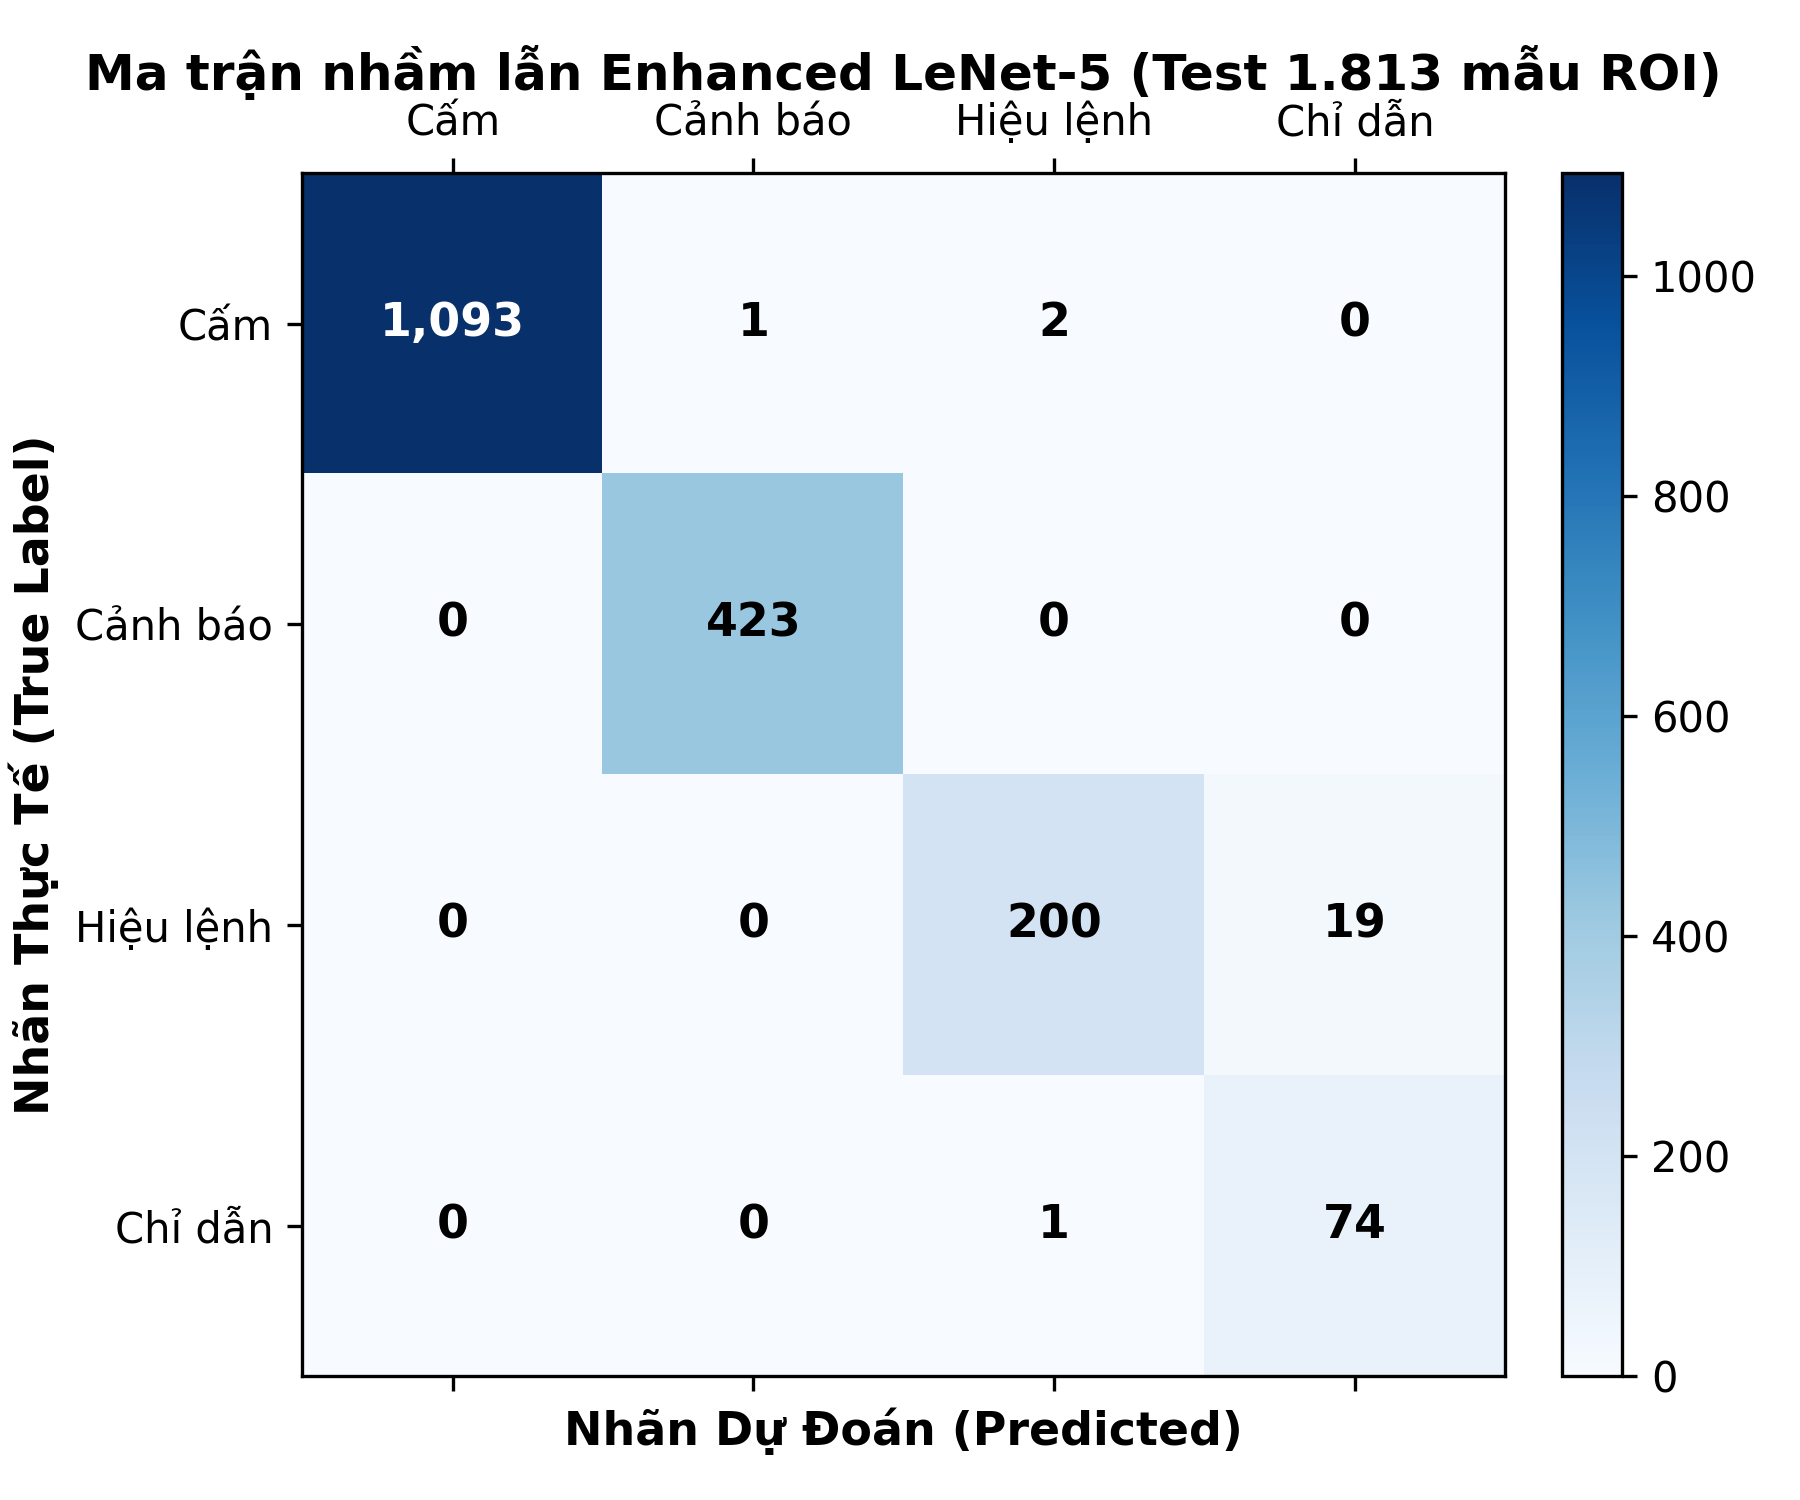
\includegraphics[width=0.58\textwidth]{graphics/sec4/f3_03_lenet_confusion_matrix.png}
\caption{Ma trận nhầm lẫn của mô hình Enhanced LeNet-5 trên tập Blind Test Block Split (1.813 mẫu ROI).}
\label{fig:lenet_confusion_matrix}
\end{figure}

\textbf{Đọc Hình~\ref{fig:lenet_confusion_matrix}:}
Ma trận nhầm lẫn của Enhanced LeNet-5 trên 1.813 mẫu test độc lập khẳng định sự vượt trội: nhóm Biển Cảnh Báo đạt độ chính xác tuyệt đối \textbf{100.0\%} (423/423 mẫu), Biển Cấm đạt \textbf{99.73\%} (1.093/1.096 mẫu). Đối với bài toán khó phân biệt giữa Biển Hiệu Lệnh và Biển Chỉ Dẫn (cùng màu xanh lam), mô hình phân loại đúng \textbf{200 / 219} mẫu Hiệu Lệnh và \textbf{74 / 75} mẫu Chỉ Dẫn, chỉ nhầm lẫn tổng cộng 20 mẫu cự ly xa bị nhòe mờ. Kết quả này bổ trợ hoàn hảo cho phân tích ma trận nhầm lẫn SVM tại Hình~\ref{fig:confusion_matrices_levels}.

\subsection{Kết quả thực nghiệm Tầng 2: Đánh giá toàn trình trên ảnh hiện trường (End-to-End Scene Benchmark)}
\label{subsec:benchmark_scene}

Thực nghiệm toàn trình được tiến hành trên \textbf{550 ảnh đường phố toàn cảnh} thuộc tập Blind Test, mô phỏng đúng luồng vận hành thực tế ngoài đường phố:

\begin{table}[H]
\centering
\small
\caption{Kết quả đối chuẩn toàn trình trên 550 ảnh đường phố toàn cảnh.}
\label{tab:scene_benchmark}
\begin{tabularx}{\textwidth}{|p{3.8cm}|p{2.2cm}|p{3.5cm}|>{\centering\arraybackslash}p{2.8cm}|>{\centering\arraybackslash}X|}
\hline
\textbf{Pipeline Toàn Trình} & \textbf{Bộ Định vị} & \textbf{Bộ Phân loại} & \textbf{Detection Recall} & \textbf{Acc $\mid$ Detection} \\
\hline
Two-Stage LeNet & YOLO11s & Enhanced LeNet-5 & 85.61\% & 99.40\% \\
\hline
Two-Stage SVM & YOLO11s & SVM (RBF) & 85.61\% & 99.17\% \\
\hline
\end{tabularx}
\end{table}

\textbf{Ý nghĩa của chỉ số đối chuẩn kép:} Việc đánh giá tách biệt hai tầng làm sáng tỏ một sự thật kỹ thuật quan trọng: Khi một biển báo đã được định vị thành công, cả hai bộ phân loại đều đạt độ chính xác gần như hoàn hảo ($\ge 99.17\%$). Điểm nghẽn hạn chế hiệu năng toàn hệ thống (End-to-End Recall $\approx 85\%$) nằm ở khâu định vị cự ly xa của YOLO11s chứ không phải do khâu phân loại.

\subsection{Chương trình Demo thực tế và các điểm sáng tạo khác biệt}
\label{subsec:demo_va_sang_tao}

\subsubsection{Ứng dụng Web tương tác hoàn chỉnh (\texttt{app\_streamlit.py})}
\label{subsubsec:demo_streamlit}

Nhóm đã xây dựng một giao diện người dùng hoàn chỉnh trên nền tảng Streamlit (\texttt{app\_streamlit.py}) phục vụ kiểm thử trực quan với các tính năng chuyên sâu:

\begin{itemize}
    \item \textbf{Chế độ ROI Side-by-Side:} Cho phép người dùng tải lên ảnh biển báo bất kỳ, trực quan hóa và so sánh song song kết quả dự đoán, phân phối xác suất và độ trễ mili-giây giữa Enhanced LeNet-5 và SVM.
    \item \textbf{Chế độ Scene Detection:} Tải lên ảnh toàn cảnh độ phân giải cao, hệ thống tự động khoanh vùng hộp bao phát hiện, cắt ROI và hiển thị nhãn phân loại theo mã màu QCVN trực quan.
    \item \textbf{Bảng tổng hợp Leaderboard:} Trực quan hóa số liệu thực nghiệm và biểu đồ đối chuẩn toàn diện của toàn bộ hệ thống.
\end{itemize}

\subsubsection{Giao diện dòng lệnh chuẩn hóa (\texttt{app.py})}
\label{subsubsec:demo_cli}

Cung cấp các lệnh kiểm thử tự động phục vụ tự động hóa và tích hợp CI/CD:
\begin{itemize}
    \item \texttt{python app.py --mode evaluate}: Tự động chạy đối chuẩn phân loại trên tập ROI kiểm thử.
    \item \texttt{python app.py --mode evaluate-scene}: Chạy pipeline đánh giá toàn trình trên 550 ảnh toàn cảnh hiện trường.
    \item \texttt{python app.py --mode demo --image path/to/image.jpg}: Chạy suy luận trực quan trên một ảnh duy nhất.
\end{itemize}

\subsubsection{Các đóng góp sáng tạo cốt lõi so với tài liệu tham khảo}
\label{subsubsec:dong_gop_sang_tao}

\begin{enumerate}
    \item \textbf{Cơ chế phân chia Block Split:} Triệt tiêu hoàn toàn hiện tượng rò rỉ dữ liệu (Data Leakage) trong video hành trình mà phần lớn các bài báo nghiên cứu trước đây thường bỏ qua khi áp dụng Random Split.
    \item \textbf{Khắc phục bài toán "Cùng màu khác hình":} Kết hợp HOG với Spatial Grid giải quyết triệt để sự nhầm lẫn giữa Biển Hiệu Lệnh (xanh tròn) và Biển Chỉ Dẫn (xanh chữ nhật/vuông).
    \item \textbf{Khung đối chuẩn công bằng (Benchmarking Framework):} Cố định tập test độc lập, chuẩn hóa kích thước đầu vào và đo kiểm song song trên cùng một môi trường phần cứng CPU chuẩn mực.
\end{enumerate}

\section{Những nhận xét và kết luận rút ra của học viên}
\label{sec:ket_luan}

\subsection{Nhận xét và kết luận kỹ thuật}
\label{subsec:nhan_xet_ky_thuat}

\begin{enumerate}
    \item \textbf{Tính ưu việt của kiến trúc phân tách trách nhiệm (Decoupling):} Việc kết hợp Deep Learning ở khâu phát hiện (YOLO11s) và các mô hình gọn nhẹ ở khâu phân loại (Enhanced LeNet-5 hoặc SVM) là giải pháp tối ưu cho các thiết bị biên, giúp đạt độ chính xác phân loại $> 98.5\%$ với tốc độ siêu nhanh trên CPU ($1.10\text{ ms}$ với LeNet-5 và $2.63\text{ ms}$ với SVM).
    \item \textbf{Tương quan giữa Học sâu và Thị giác máy tính truyền thống:}
    \begin{itemize}
        \item \textit{Enhanced LeNet-5 (Học sâu):} Chiếm ưu thế về độ chính xác ($98.73\%$ vs $98.57\%$), Macro-F1 ($95.66\%$ vs $95.51\%$) và tốc độ suy luận ($1.10\text{ ms}$ vs $2.63\text{ ms}$). Mạng nơ-ron tự động biểu diễn được các hoa văn tinh xảo trong biển báo mà không cần căn chỉnh tham số trích xuất thủ công.
        \item \textit{Color + HOG + SVM (Truyền thống):} Vẫn chứng minh sức mạnh đáng nể ($98.57\%$ Accuracy) với ưu điểm lớn về tính minh bạch toán học (Explainability), dễ diễn giải và không đòi hỏi quá trình huấn luyện phức tạp.
    \end{itemize}
\end{enumerate}

\subsection{Các hạn chế kỹ thuật hiện tại}
\label{subsec:han_che}

\begin{enumerate}
    \item \textbf{Hạn chế phát hiện ở cự ly xa:} YOLO11s còn bỏ sót $14.39\%$ biển báo trên tập test. Phần lớn các trường hợp bỏ sót rơi vào biển báo ở khoảng cách rất xa, kích thước trên ảnh chỉ dưới $15\text{ px}$, nơi tín hiệu biên cạnh bị tiêu biến qua các tầng downsampling của mạng.
    \item \textbf{Biến thiên ánh sáng phức tạp:} Không gian màu HSV có thể bị dao động trong các điều kiện thời tiết khắc nghiệt như mưa lớn gây lóa đèn vào ban đêm hoặc bóng râm gắt che một nửa mặt biển.
    \item \textbf{Giới hạn một lần chạy và một hạt ngẫu nhiên (Single Seed):} Toàn bộ các thực nghiệm huấn luyện detector YOLO11s và các mô hình phân loại truyền thống đều mới được tiến hành trên 1 lần chạy duy nhất với 1 hạt ngẫu nhiên cố định ($\text{seed} = 0$ hoặc $\text{seed} = 42$), chưa kiểm chứng độ ổn định và phương sai qua nhiều seed khác nhau.
    \item \textbf{Đặc thù tương quan chuỗi khung hình (Temporal Correlation):} Dù tập kiểm thử chứa tới 1.821 bounding box biển báo, các khung hình này được trích xuất từ các chuỗi video hành trình liên tục nên thực chất chỉ tương ứng với khoảng \textbf{161 biển báo vật lý độc lập (tracks)}. Do đó, sự thiếu hụt các đối tượng vật lý độc lập khiến cho một số sai lệch cục bộ lặp lại trong chuỗi (chẳng hạn 19 frame lệch hộp của một cột biển cấm P.130) bị phóng đại lên trong bảng thống kê tổng thể.
    \item \textbf{Hiện tượng nhãn thiếu trong Ground Truth thực tế (Missing Annotations):} Khảo sát mẫu 20 trường hợp báo động giả (False Positive) có độ tự tin cao nhất của detector \texttt{vn\_s} ghi nhận có tới \textbf{12/20 trường hợp (chiếm 60\% mẫu khảo sát)} thực chất là biển báo giao thông có thật ngoài đời thực bị người gán nhãn bỏ sót trong tập dữ liệu gốc. Hiện tượng thiếu nhãn này làm suy giảm chỉ số Precision và mAP thực nghiệm nhưng hoàn toàn không làm thay đổi giá trị Recall kiểm chứng trên các biển đã có nhãn ground-truth.
    \item \textbf{Điểm mù hoàn toàn đối với nhóm biển phụ:} Cả 3 biến thể detector YOLO11s đều đạt Recall \textbf{0.0\% (0/8 mẫu)} đối với nhóm biển phụ (mã S.505a) do kích thước siêu nhỏ, dạng chữ nhật dẹt nằm sát mép dưới biển chính dẫn tới việc detector không phân tách được biên giới hộp bao. Cỡ mẫu quá nhỏ ($n=8$) cũng khiến việc đánh giá phân loại nhóm này chưa đủ ý nghĩa thống kê tin cậy.
    \item \textbf{Bỏ sót hoàn toàn 37 biển báo vật lý (Tracks):} Có \textbf{37 / 161 biển báo vật lý} trên đường không có bất kỳ khung hình nào được phát hiện bởi detector \texttt{vn\_s} (kích thước tối đa trung bình của chuỗi vết này chỉ đạt $\approx 20.8\text{ px}$), chủ yếu rơi vào các tình huống bị tán cây rậm che khuất, nằm hoàn toàn trong vùng bóng râm tối hoặc biển bị gỉ sét, biến dạng nặng.
    \item \textbf{Cảnh báo suy diễn thống kê trên các phân nhóm cỡ mẫu nhỏ:} Đối với các nhóm hoặc mã hiệu có số lượng mẫu kiểm thử rất ít (như nhóm biển phụ hoặc một số mã biển chỉ dẫn hiếm), nhóm nghiên cứu không rút ra kết luận mang tính khái quát hóa tuyệt đối mà chỉ ghi nhận hiện tượng thực nghiệm tại chỗ.
\end{enumerate}

\subsection{Hướng phát triển trong tương lai}
\label{subsec:huong_phat_trien}

\begin{enumerate}
    \item \textbf{Ứng dụng kỹ thuật SAHI (Slicing Aided Hyper Inference):} Chia nhỏ ảnh lớn thành các ô trượt nhằm nâng cao độ nhạy phát hiện đối với các biển báo siêu nhỏ ở cự ly xa.
    \item \textbf{Phân loại phân cấp 52 mã hiệu chi tiết (Hierarchical Classification):} Mở rộng từ bài toán nhận diện 4 nhóm quy chuẩn sang nhận dạng chính xác từng mã hiệu biển báo cụ thể trong QCVN 41:2019.
\end{enumerate}

\newpage
\renewcommand{\refname}{Tài liệu tham khảo}
\begin{thebibliography}{99}
\addcontentsline{toc}{section}{Tài liệu tham khảo}

\bibitem{qcvn41} Bộ Giao thông Vận tải, \emph{Quy chuẩn kỹ thuật quốc gia về báo hiệu đường bộ (QCVN 41:2019/BGTVT)}, Nhà xuất bản Giao thông Vận tải, Hà Nội, 2019.

\bibitem{dalal2005} N. Dalal and B. Triggs, ``Histograms of oriented gradients for human detection,'' in \emph{IEEE Computer Society Conference on Computer Vision and Pattern Recognition (CVPR)}, vol. 1, pp. 886--893, 2005.

\bibitem{lecun1998} Y. LeCun, L. Bottou, Y. Bengio, and P. Haffner, ``Gradient-based learning applied to document recognition,'' \emph{Proceedings of the IEEE}, vol. 86, no. 11, pp. 2278--2324, 1998.

\bibitem{cortes1995} C. Cortes and V. Vapnik, ``Support-vector networks,'' \emph{Machine Learning}, vol. 20, no. 3, pp. 273--297, 1995.

\bibitem{ioffe2015} S. Ioffe and C. Szegedy, ``Batch normalization: Accelerating deep network training by reducing internal covariate shift,'' in \emph{International Conference on Machine Learning (ICML)}, pp. 448--456, 2015.

\bibitem{srivastava2014} N. Srivastava, G. Hinton, A. Krizhevsky, I. Sutskever, and R. Salakhutdinov, ``Dropout: A simple way to prevent neural networks from overfitting,'' \emph{Journal of Machine Learning Research (JMLR)}, vol. 15, no. 1, pp. 1929--1958, 2014.

\bibitem{kingma2015} D. P. Kingma and J. Ba, ``Adam: A method for stochastic optimization,'' in \emph{International Conference on Learning Representations (ICLR)}, 2015.

\bibitem{yolo11} G. Jocher, A. Chaurasia, and J. Qiu, ``Ultralytics YOLO11,'' 2024. [Online]. Available: \url{https://github.com/ultralytics/ultralytics}.

\bibitem{uit_cs231} Trường Đại học Công nghệ Thông tin -- ĐHQG-HCM, \emph{Phiếu đánh giá đồ án môn học Thị giác máy tính (CS231)}, TP.HCM, 2026.

\end{thebibliography}


\end{document}
